\section{Properties of the Benchmark}

\begin{figure*}[h]
\begin{center}
$$ 
\begin{bmatrix}
\frac{1}{2} & -\frac{1}{2} & \frac{1}{2} & -\frac{1}{2} & \frac{1}{2} & -\frac{1}{2}  \\
-\frac{1}{2} & \frac{1}{2} & \frac{1}{2} & -\frac{1}{2} & \frac{1}{2} & -\frac{1}{2} \\
\frac{1}{2} & -\frac{1}{2} & -\frac{1}{2} & \frac{1}{2} & \frac{1}{2} & -\frac{1}{2}  \\
-\frac{1}{2} & \frac{1}{2} & -\frac{1}{2} & \frac{1}{2} & \frac{1}{2} & -\frac{1}{2} \\
\frac{1}{2} & -\frac{1}{2} & \frac{1}{2} & -\frac{1}{2} & -\frac{1}{2} & \frac{1}{2}  \\
-\frac{1}{2} & \frac{1}{2} & \frac{1}{2} & -\frac{1}{2} & -\frac{1}{2} & \frac{1}{2}  \\
\frac{1}{2} & -\frac{1}{2} & -\frac{1}{2} & \frac{1}{2} &-\frac{1}{2} & \frac{1}{2} \\
-\frac{1}{2} & \frac{1}{2} & -\frac{1}{2} & \frac{1}{2}  & -\frac{1}{2} & \frac{1}{2} \\
\end{bmatrix} ~~~~~~~~
\begin{bmatrix}
 \frac{2}{3}   & -\frac{1}{3}  & -\frac{1}{3} & \frac{2}{3}   & -\frac{1}{3}  & -\frac{1}{3}   \\
 -\frac{1}{3}  & \frac{2}{3}   & -\frac{1}{3} & \frac{2}{3}   & -\frac{1}{3}  & -\frac{1}{3}   \\
 -\frac{1}{3}  & -\frac{1}{3}  & \frac{2}{3}  & \frac{2}{3}   & -\frac{1}{3}  & -\frac{1}{3}   \\
 \frac{2}{3}   & -\frac{1}{3}  & -\frac{1}{3} & -\frac{1}{3}  & \frac{2}{3}   & -\frac{1}{3}   \\
 -\frac{1}{3}  & \frac{2}{3}   & -\frac{1}{3} & -\frac{1}{3}  & \frac{2}{3}   & -\frac{1}{3}   \\
 -\frac{1}{3}  & -\frac{1}{3}  & \frac{2}{3}  & -\frac{1}{3}  & \frac{2}{3}   &  -\frac{1}{3}  \\
 \frac{2}{3}   & -\frac{1}{3}  & -\frac{1}{3} & -\frac{1}{3}  & -\frac{1}{3}  & \frac{2}{3}    \\
 -\frac{1}{3}  & \frac{2}{3}   & -\frac{1}{3} & -\frac{1}{3}  & -\frac{1}{3}  & \frac{2}{3}    \\
 -\frac{1}{3}  & -\frac{1}{3}  & \frac{2}{3}  & -\frac{1}{3}  & -\frac{1}{3}  & \frac{2}{3}    \\
\end{bmatrix} 
$$
\end{center}
\caption{Benchmark construction for $k=2$ and $\alpha=3$ (left) and $k=3$ and $\alpha=2$ (right).}
\label{fig:benchmark-small-instances}
\end{figure*}


\begin{fact}
For $a\neq a'$, we have $d(\mathcal{C}^{a},\mathcal{C}^{a'}) = 1-1/k$.
\end{fact}
\begin{proof}
Consider an arbitrary vector $v_i^{\ell}$. By construction, the positive entries of $v_i^{\ell}$ range from $k^{\ell-1}\cdot i+1$ to $k^{\ell-1}\cdot (i+1)$. Similarly, the positive entries for the vector $v_j^{\ell-1}$ range from range from $k^{\ell-2}\cdot j+1$ to $k^{\ell-2}\cdot (j+1)$. Therefore, concatenating $v_j^{\ell-1}$ $k$ times into a vector $v'$, $v'$ and $v_i^{\ell}$ can share at most one positive coordinate. Inductively, the same holds true for any concatenation of vectors $v_j^{\ell-h}$.
Thus, the two clusters induced by the columns formed by concatenating the vectors $v$ can share only a $1/k$ fraction of the points. Since each cluster consists of exactly $k^{\alpha}/k$ = $k^{\alpha-1}$ points, the confusion matrix $M$ only has entries $\frac{n}{k^2}$ and for any permutation $\pi$, we have $d(\mathcal{C}^{a},\mathcal{C}^{a'}) = 1-1/k$.
\end{proof}

\begin{fact}
\label{fact:cost}
For any $C_j^a$, we have $\cost_{C_j^a}(\{\mu(C_j^a)\}) = (\alpha-1)\cdot k^{\alpha-2}\cdot (k-1)$.
\end{fact}
\begin{proof}
Without loss of generality, we consider $C_1^0$; the proof is analogous for the other choices of $j$ and $a$. We first note that for any point $A_i \in C_1^0$, the coordinates $A_{i,\ell}$ are identical for $\ell <k$. Furthermore for the column $\ell\geq k$, we have by construction $\sum_{A_i\in C_j} A_{i,\ell} = k^{\alpha-1}\cdot \frac{k-1}{k} + (k^{\alpha}-k^{\alpha-1})\frac{1}{k}=k^{\alpha-1}\cdot (\frac{k-1}{k} - (k-1)\frac{1}{k}) = 0.$ Therefore, the mean of $C_1^0$ satisfies $\mu(C_1^0)_{\ell} = \begin{cases}A_{i,\ell} &\text{if }\ell<k \\
0 &\text{else.}\end{cases}$. 
Thus, the cost is precisely $(\alpha-1)\cdot k^{\alpha-1}\cdot \left(\left(\frac{k-1}{k}\right)^2 + \left(\frac{1}{k}\right)^2 \right)=(\alpha-1)\cdot k^{\alpha-2}\cdot (k-1)$.
\end{proof}

Finally, we show that the means for the clustering $\mathcal{C}^{a}$ also induce $\mathcal{C}^{a}$.

\begin{fact}
\label{fact:opt}
For a clustering $\mathcal{C}^{a}$, let $\mu(C_j^{a})$ denote the mean of cluster $C_j^a$. Then every point  is assigned to its closest center. Moreover, every point $A_i$ of $C_j^a$ has equal distance to any center $\mu(C_h^{a})$ with $h\neq j$.
\end{fact}
\begin{proof}
Again, we assume without loss of generality $a=0$.
Let $A_i$ be an arbitrary point of cluster $C_{h}^{a}$ and consider the mean $\mu(C_j^a)_{\ell} = \begin{cases}A_{i,\ell} &\text{if }\ell<k \\
0 &\text{else.}\end{cases}$ of cluster $C_j^a$. By definition, the positive coordinates of $A_i$ are not equal to the positive coordinates of $\mu(C_j^a)$. The only difference in coordinates between the means of $\mu(C_j^a)$ and $\mu(C_h^a)$ are the first $k$ coordinates, as the rest are $0$.
But here the coordinates of $\mu(C_h^a)$ and $A_i$ are identical, hence $\mu(C_j^a)$ cannot be closer to $A_i$.

To prove that the distances between $A_i$ and any $\mu(C_h^{a})$ with $h\neq j$ are equal, again consider that any difference can only exist among the first $k$ coordinates. Here, we have $\mu(C_h^{a})_h = \frac{k-1}{k}$, and the remaining columns are $-\frac{1}{k}$. Since $A_{i,h} = -\frac{1}{k}$ for any $h\neq j$, the claim follows.
\end{proof}

\section{Hardness of Weak Coreset Evaluation}

Here, we show that it is in general co-NP hard to evaluate whether two point sets $A$ and $B$ are weak coresets of each other. A weak coreset only requires that a $(1+\varepsilon)$ approximation for one point set is a $(1+O(\varepsilon))$ for the other.


\begin{proposition}
\label{prop:hardness}
Given two point sets $A$ and $B$ in $\mathbb{R}^d$ and a sufficiently small (constant) $\varepsilon>0$, it is co-NP hard to decide whether $A$ is a weak coreset of $B$.
\end{proposition}
\begin{proof}
First, we recall that for some $\varepsilon_0$ and candidate clustering cost $V$, it is NP-hard to decide whether there exists a clustering $C$ with cost in $\cost_A(C)\leq V$ and $\cost_B(C)\geq (1+\varepsilon_0)\cdot V$.
Conversely, it is co-NP-hard to decide whether there exists no set of centers $C$ such that $\cost_A(C)\leq V$ and $\cost_B(C) \geq (1+\varepsilon_0)\cdot V$.
\end{proof}

We remark that the possible values for $\varepsilon_0$ are determined by the current APX-hardness results. Assuming NP$\neq$P, $\varepsilon_0\approx 1.07$ and assuming UCG, $\varepsilon_0 \approx 1.17$~\cite{Cohen-AddadSL21,Cohen-AddadS19} for $k$-means in Euclidean spaces.



\paragraph*{Further Extensions}

On the benchmark we considered here, both Sensitivity Sampling, as well as Group Sampling are similar to uniform sampling and, indeed, uniform sampling could be used to construct a good coreset. We can eliminate uniform sampling as a viable algorithm for this instance by combining multiple benchmarks $B_1,\ldots B_t$ with $\sum_{i=1}^t  k_i =k$. Each benchmark then has size $\sum_{i=1}^t  k_i^{\alpha}$. We then add an additive offset to the coordinates of each benchmark such that they do not interfere. In this case, uniform sampling does not work if the values of the $k_i$ are different enough. Since it is well known that uniform sampling is not a viable coreset algorithm in both theory and practice, we only used the basic benchmark for our evaluations.





\section{Details on the Real World Data Sets}
\label{sec:real-world-datasets-details}

The \textit{Census}\footnote{\url{https://archive.ics.uci.edu/ml/datasets/US+Census+Data+(1990)}} dataset is a small subset of the Public Use Microdata Samples from 1990 US census. It consists of demographic information encoded as 68 categorical attributes of 2,458,285 individuals. 

\textit{Covertype}\footnote{\url{https://archive.ics.uci.edu/ml/datasets/covertype}} is comprised of cartographic descriptions and forest cover type of four wilderness areas in the Roosevelt National Forest of Northern Colorado in the US. It consists of 581,012 records, 54 cartographic variables and one class variable. Although \textit{Covertype} was originally made for classification tasks, it is often used for clustering tasks by removing the class variable~\cite{AckermannMRSLS12}.

The data set with the fewest number of dimensions is \textit{Tower}\footnote{\url{http://homepages.uni-paderborn.de/frahling/coremeans.html}}. This data set consists of 4,915,200 rows and 3 features as it is a 2,560 by 1,920 picture of a tower on a hill where each pixel is represented by a RGB color value. 

Inspired by~\cite{FGSSS13}, \textit{Caltech} was created by computing SIFT features from the images in the Caltech101\footnote{\url{http://www.vision.caltech.edu/Image_Datasets/Caltech101/}} image database. This database contains pictures of objects partitioned into 101 categories. Disregarding the categories, we concatenated the 128-dimensional SIFT vectors from each image into one large data matrix with 3,680,458 rows and 128 columns. 

\textit{NYTimes}\footnote{\url{https://archive.ics.uci.edu/ml/datasets/bag+of+words}} is a dataset composed of the bag-of-words (BOW) representations of 300,000 news articles from The New York Times. The vocabulary size of the text collection is 102,660. Due to the BOW encoding, \textit{NYTimes} has a very large number of dimensions and is highly sparse. To make processing feasible, we reduced the number of dimensions to 100 using terminal embeddings.





\section{A Brief Introduction to Dimension Reduction for Coresets}
There are essentially two main dimension reduction techniques for coresets.

{\bf Principal Component Analysis:} Feldman, Schmidt, and Sohler~\cite{FSS13} showed that projecting an input $A$ onto the first $O(k/\varepsilon^2)$ principal components is a coreset, albeit in low dimension. The analysis was subsequently tightened by~\cite{CEMMP15} and extended to other center-based cost functions by~\cite{SohlerW18}. Although its target dimension is generally worse than those based on random projections and terminal embeddings, there is nevertheless reasons for using PCA regardless: It removes noise and thus may make it easier to compute a high quality coreset.

{\bf Terminal Embeddings:} Given a set of points $A$ in $\mathbb{R}^D$, a terminal embedding $f:\mathbb{R}^D\rightarrow \mathbb{R}^d$ preserves the pairwise distance between any point $p\in A$ and any point $q\in \mathbb{R}^D$ up to a $(1\pm \varepsilon)$ factor. The statement is related to the famous Johnson-Lindenstrauss lemma but it is stronger as it does not apply to only the pairwise distances of $A$. Nevertheless, the same target dimension is sufficient. Terminal embeddings were studied by~\cite{ElkinFN17,MahabadiMMR18,NaN18}, with Narayanan and Nelson \cite{NaN18} achieving an optimal target dimension of $O(\varepsilon^{-2}\log n)$, where $n$ is the number of points. For applications to coresets, we refer to \cite{BecchettiBC0S19,Cohen-AddadSS21,huang2020coresets}.

For an overview on practical aspects of dimension reduction, we refer to Venkatsubramanian and Wang~\cite{VenkatasubramanianW11}. The performance of the algorithms when applying a Johnson-Lindenstrauss transformation does not affect the behaviour of an algorithm that only depends on pairwise distances. Thus terminal embeddings are mainly used in the analysis of an algorithm, rather than as an explicit preprocessing step.
We note that terminal embeddings, combined with an iterative application of the coreset construction from \cite{BravermanJKW21}, can reduce the target dimension to a factor $\tilde{O}(\varepsilon^{-2} \log k)$. This is mainly of theoretical interest, as in practice the deciding factor wrt the target dimension is the precision, rather than dependencies on $\log n$ and $\log k$.







\section{Distortions}
\label{sec:distortions-tables}

The tables 
(\cref{tab:distortions-mean-std-benchmark},
 \cref{tab:distortions-mean-std-caltech},
 \cref{tab:distortions-mean-std-caltech-pca},
 \cref{tab:distortions-mean-std-census},
 \cref{tab:distortions-mean-std-census-pca},
 \cref{tab:distortions-mean-std-covertype},
 \cref{tab:distortions-mean-std-covertype-pca},
 \cref{tab:distortions-mean-std-nytimes},
 \cref{tab:distortions-mean-std-nytimes-pca},
 \cref{tab:distortions-mean-std-tower})
show the distortions of the 5 evaluated algorithms on the different data sets.
We vary the coreset size $T$ for different $k$ values using the formula: $T=mk$ where $m = \{50, 100, 200, 500\}$.
The running time for StreamKM++ with coreset size $T=500k$ exceeds the allocated time budget of 32 hours on almost all data sets.
For this reason, the distortions for StreamKM++ with $m=500$ are not present in the tables.



\begin{longtable}{lllllll}
\multicolumn{7}{c}{\textbf{Distortions on the \textit{Caltech} data set}} \\
\toprule
\parbox[t]{5mm}{\ \\$k$} 
& \parbox[t]{5mm}{\ \\$m$} 
& BICO 
& \parbox[t]{1.7cm}{Group\\Sampling} 
& \parbox[t]{1.7cm}{Ray\\Maker}
& \parbox[t]{1.7cm}{Sensitivity\\Sampling}
&    StreamKM++ \\
\midrule
10 & 50  &  3.40 (0.440) &   1.02 (0.010) &  5.05 (0.157) &         1.02 (0.005) &  1.07 (0.005) \\
   & 100 &  3.24 (0.729) &   1.01 (0.004) &  3.84 (0.081) &         1.01 (0.003) &  1.05 (0.004) \\
   & 200 &  2.90 (0.153) &   1.01 (0.002) &  3.48 (0.052) &         1.01 (0.002) &  1.04 (0.002) \\
   & 500 &  2.62 (0.095) &   1.01 (0.001) &  3.40 (0.058) &         1.00 (0.001) &  \\
 \midrule
20 & 50  &  3.22 (0.160) &   1.04 (0.004) &  5.52 (0.266) &         1.02 (0.003) &  1.08 (0.006) \\
   & 100 &  3.09 (0.122) &   1.02 (0.004) &  4.31 (0.130) &         1.01 (0.002) &  1.08 (0.003) \\
   & 200 &  2.88 (0.078) &   1.01 (0.002) &  3.93 (0.120) &         1.01 (0.001) &  1.11 (0.002) \\
   & 500 &  2.36 (0.051) &   1.01 (0.001) &  3.81 (0.116) &         1.01 (0.001) &  \\
 \midrule
30 & 50  &  2.81 (0.244) &   1.03 (0.006) &  6.43 (0.470) &         1.02 (0.002) &  1.13 (0.004) \\
   & 100 &  2.58 (0.105) &   1.02 (0.003) &  4.65 (0.256) &         1.02 (0.002) &  1.13 (0.004) \\
   & 200 &  2.38 (0.098) &   1.01 (0.002) &  4.12 (0.234) &         1.01 (0.002) &  1.10 (0.002) \\
   & 500 &  2.01 (0.065) &   1.01 (0.001) &  4.00 (0.138) &         1.01 (0.001) &  \\
 \midrule
40 & 50  &  3.16 (0.500) &   1.03 (0.004) &  5.62 (0.287) &         1.02 (0.004) &  1.10 (0.004) \\
   & 100 &  2.78 (0.258) &   1.02 (0.001) &  4.42 (0.200) &         1.02 (0.002) &  1.14 (0.003) \\
   & 200 &  2.79 (0.217) &   1.02 (0.001) &  3.82 (0.111) &         1.01 (0.001) &  1.17 (0.004) \\
   & 500 &  2.57 (0.113) &   1.01 (0.001) &  3.86 (0.122) &         1.01 (0.001) &            \\
\bottomrule
\caption{Distortions of the evaluated algorithms on the \textit{Benchmark} data set. Each cell specify the mean distortion along with the standard deviation in parenthesis of 10 repetitions of the experiment.}
\label{tab:distortions-mean-std-benchmark}
\end{longtable}

\begin{longtable}{lllllll}
\multicolumn{7}{c}{\textbf{Distortions on the \textit{Caltech} data set}} \\
\toprule
\parbox[t]{5mm}{\ \\$k$} 
& \parbox[t]{5mm}{\ \\$m$} 
& BICO 
& \parbox[t]{1.7cm}{Group\\Sampling} 
& \parbox[t]{1.7cm}{Ray\\Maker}
& \parbox[t]{1.7cm}{Sensitivity\\Sampling}
&    StreamKM++ \\
\midrule
10 & 50  &  5.12 (0.307) &   1.07 (0.009) &  7.05 (0.250) &         1.05 (0.013) &  1.16 (0.008) \\
   & 100 &  4.48 (0.284) &   1.04 (0.006) &  5.46 (0.254) &         1.03 (0.008) &  1.13 (0.005) \\
   & 200 &  4.08 (0.319) &   1.02 (0.004) &  5.00 (0.196) &         1.01 (0.005) &  1.10 (0.005) \\
   & 500 &  3.41 (0.215) &   1.01 (0.003) &  4.75 (0.188) &         1.00 (0.003) &  \\
 \midrule
20 & 50  &  6.35 (1.173) &   1.06 (0.008) &  6.92 (0.209) &         1.05 (0.007) &  1.18 (0.008) \\
   & 100 &  4.65 (0.283) &   1.04 (0.005) &  5.29 (0.146) &         1.03 (0.005) &  1.14 (0.005) \\
   & 200 &  4.19 (0.384) &   1.02 (0.002) &  4.80 (0.112) &         1.01 (0.004) &  1.12 (0.004) \\
   & 500 &  3.50 (0.404) &   1.01 (0.002) &  4.61 (0.096) &         1.00 (0.001) &  \\
 \midrule
30 & 50  &  6.01 (0.335) &   1.06 (0.005) &  6.79 (0.149) &         1.04 (0.004) &  1.19 (0.005) \\
   & 100 &  5.10 (0.628) &   1.04 (0.005) &  5.30 (0.123) &         1.02 (0.005) &  1.15 (0.002) \\
   & 200 &  4.29 (0.659) &   1.02 (0.003) &  4.70 (0.075) &         1.01 (0.003) &  1.13 (0.002) \\
   & 500 &  3.09 (0.138) &   1.01 (0.002) &  4.62 (0.090) &         1.00 (0.002) &  \\
 \midrule
40 & 50  &  6.24 (0.524) &   1.07 (0.004) &  6.85 (0.145) &         1.05 (0.004) &  1.20 (0.004) \\
   & 100 &  5.23 (0.874) &   1.04 (0.003) &  5.22 (0.092) &         1.02 (0.002) &  1.16 (0.003) \\
   & 200 &  4.50 (1.085) &   1.02 (0.002) &  4.72 (0.086) &         1.01 (0.001) &  1.13 (0.002) \\
   & 500 &  3.38 (0.398) &   1.01 (0.001) &  4.55 (0.094) &         1.00 (0.001) &  \\
 \midrule
50 & 50  &  7.50 (1.013) &   1.07 (0.004) &  6.80 (0.092) &         1.05 (0.004) &  1.20 (0.006) \\
   & 100 &  5.21 (0.968) &   1.04 (0.003) &  5.18 (0.084) &         1.03 (0.002) &  1.16 (0.005) \\
   & 200 &  4.21 (0.296) &   1.02 (0.002) &  4.69 (0.065) &         1.01 (0.003) &  1.13 (0.002) \\
   & 500 &  3.36 (0.429) &   1.01 (0.001) &  4.52 (0.058) &         1.00 (0.001) &            \\
\bottomrule
\caption{Distortions of the evaluated algorithms on the \textit{Caltech} data set. Each cell specify the mean distortion along with the standard deviation in parenthesis of 10 repetitions of the experiment.}
\label{tab:distortions-mean-std-caltech}
\end{longtable}

\begin{longtable}{lllllll}
\multicolumn{7}{c}{\textbf{Distortions on the \textit{Caltech} data set (with PCA preprocessing)}} \\
\toprule
\parbox[t]{5mm}{\ \\$k$} & \parbox[t]{5mm}{\ \\$m$} &BICO & \parbox[t]{1.7cm}{Group\\Sampling} &\parbox[t]{1.7cm}{Ray\\Maker}&\parbox[t]{1.7cm}{Sensitivity\\Sampling}&    StreamKM++ \\
\midrule
10 & 50  &  1.21 (0.009) &   1.03 (0.004) &  1.25 (0.005) &         1.02 (0.007) &  1.04 (0.005) \\
   & 100 &  1.19 (0.006) &   1.02 (0.006) &  1.21 (0.006) &         1.01 (0.004) &  1.03 (0.004) \\
   & 200 &  1.16 (0.003) &   1.01 (0.002) &  1.19 (0.003) &         1.01 (0.003) &  1.02 (0.002) \\
   & 500 &  1.13 (0.007) &   1.00 (0.002) &  1.19 (0.006) &         1.00 (0.001) &  \\
 \midrule
20 & 50  &  1.54 (0.024) &   1.04 (0.006) &  1.63 (0.008) &         1.03 (0.006) &  1.07 (0.003) \\
   & 100 &  1.48 (0.020) &   1.02 (0.002) &  1.54 (0.010) &         1.01 (0.004) &  1.06 (0.003) \\
   & 200 &  1.41 (0.006) &   1.01 (0.002) &  1.50 (0.011) &         1.01 (0.003) &  1.04 (0.003) \\
   & 500 &  1.35 (0.008) &   1.00 (0.001) &  1.49 (0.008) &         1.00 (0.001) &  \\
 \midrule
30 & 50  &  1.99 (0.032) &   1.05 (0.006) &  2.05 (0.020) &         1.03 (0.003) &  1.10 (0.004) \\
   & 100 &  1.82 (0.099) &   1.03 (0.004) &  1.90 (0.014) &         1.02 (0.003) &  1.08 (0.002) \\
   & 200 &  1.72 (0.046) &   1.01 (0.002) &  1.84 (0.009) &         1.01 (0.002) &  1.06 (0.002) \\
   & 500 &  1.62 (0.037) &   1.01 (0.001) &  1.81 (0.011) &         1.00 (0.002) &  \\
 \midrule
40 & 50  &  2.34 (0.112) &   1.05 (0.003) &  2.48 (0.020) &         1.04 (0.005) &  1.12 (0.004) \\
   & 100 &  2.25 (0.066) &   1.03 (0.003) &  2.23 (0.011) &         1.02 (0.001) &  1.09 (0.003) \\
   & 200 &  2.11 (0.072) &   1.02 (0.002) &  2.15 (0.012) &         1.01 (0.003) &  1.07 (0.002) \\
   & 500 &  1.90 (0.070) &   1.01 (0.002) &  2.12 (0.011) &         1.00 (0.001) &  \\
 \midrule
50 & 50  &  2.86 (0.214) &   1.06 (0.003) &  2.94 (0.026) &         1.04 (0.005) &  1.14 (0.005) \\
   & 100 &  2.58 (0.124) &   1.03 (0.001) &  2.59 (0.019) &         1.02 (0.001) &  1.11 (0.002) \\
   & 200 &  2.35 (0.139) &   1.02 (0.001) &  2.49 (0.021) &         1.01 (0.002) &  1.09 (0.002) \\
   & 500 &  2.15 (0.075) &   1.01 (0.001) &  2.44 (0.015) &         1.00 (0.001) &            \\
\bottomrule
\caption{Distortions of the evaluated algorithms on the \textit{Caltech} data set (with PCA preprocessing). Each cell specify the mean distortion along with the standard deviation in parenthesis of 10 repetitions of the experiment.}
\label{tab:distortions-mean-std-caltech-pca}
\end{longtable}

\begin{longtable}{lllllll}
\multicolumn{7}{c}{\textbf{Distortions on the \textit{Census} data set}} \\
\toprule
\parbox[t]{5mm}{\ \\$k$} & \parbox[t]{5mm}{\ \\$m$} &BICO & \parbox[t]{1.7cm}{Group\\Sampling} &\parbox[t]{1.7cm}{Ray\\Maker}&\parbox[t]{1.7cm}{Sensitivity\\Sampling}&    StreamKM++ \\
\midrule
10 & 50  &  2.08 (0.106) &   1.08 (0.019) &  2.30 (0.162) &         1.03 (0.031) &  1.10 (0.012) \\
   & 100 &  1.83 (0.124) &   1.04 (0.021) &  1.92 (0.094) &         1.03 (0.012) &  1.07 (0.006) \\
   & 200 &  1.65 (0.056) &   1.02 (0.005) &  1.72 (0.050) &         1.02 (0.012) &  1.05 (0.005) \\
   & 500 &  1.48 (0.053) &   1.02 (0.004) &  1.69 (0.029) &         1.02 (0.010) &  \\
 \midrule
20 & 50  &  2.18 (0.164) &   1.07 (0.022) &  2.31 (0.078) &         1.03 (0.007) &  1.10 (0.008) \\
   & 100 &  1.93 (0.080) &   1.04 (0.011) &  1.91 (0.048) &         1.02 (0.011) &  1.08 (0.005) \\
   & 200 &  1.71 (0.031) &   1.03 (0.006) &  1.75 (0.027) &         1.01 (0.006) &  1.06 (0.004) \\
   & 500 &  1.51 (0.048) &   1.02 (0.005) &  1.66 (0.019) &         1.01 (0.004) &  \\
 \midrule
30 & 50  &  2.28 (0.177) &   1.07 (0.011) &  2.38 (0.077) &         1.03 (0.011) &  1.11 (0.007) \\
   & 100 &  2.05 (0.096) &   1.04 (0.006) &  1.95 (0.040) &         1.02 (0.007) &  1.09 (0.004) \\
   & 200 &  1.76 (0.055) &   1.03 (0.005) &  1.79 (0.034) &         1.01 (0.007) &  1.07 (0.003) \\
   & 500 &  1.56 (0.016) &   1.01 (0.003) &  1.71 (0.038) &         1.01 (0.003) &  \\
 \midrule
40 & 50  &  2.47 (0.101) &   1.08 (0.009) &  2.43 (0.069) &         1.02 (0.010) &  1.12 (0.006) \\
   & 100 &  2.11 (0.104) &   1.04 (0.006) &  1.99 (0.034) &         1.01 (0.004) &  1.09 (0.003) \\
   & 200 &  1.83 (0.038) &   1.02 (0.007) &  1.81 (0.026) &         1.01 (0.005) &  1.08 (0.002) \\
   & 500 &  1.56 (0.039) &   1.01 (0.005) &  1.73 (0.026) &         1.01 (0.003) &  \\
 \midrule
50 & 50  &  2.50 (0.138) &   1.07 (0.008) &  2.48 (0.054) &         1.02 (0.011) &  1.13 (0.004) \\
   & 100 &  2.12 (0.109) &   1.04 (0.007) &  2.02 (0.055) &         1.01 (0.004) &  1.10 (0.003) \\
   & 200 &  1.84 (0.059) &   1.03 (0.004) &  1.82 (0.022) &         1.01 (0.005) &  1.08 (0.004) \\
   & 500 &  1.57 (0.019) &   1.02 (0.004) &  1.75 (0.022) &         1.01 (0.003) &            \\
\bottomrule
\caption{Distortions of the evaluated algorithms on the \textit{Census} data set. Each cell specify the mean distortion along with the standard deviation in parenthesis of 10 repetitions of the experiment.}
\label{tab:distortions-mean-std-census}
\end{longtable}

\begin{longtable}{lllllll}
\multicolumn{7}{c}{\textbf{Distortions on the \textit{Census} data set (with PCA preprocessing)}} \\
\toprule
\parbox[t]{5mm}{\ \\$k$} & \parbox[t]{5mm}{\ \\$m$} &BICO & \parbox[t]{1.7cm}{Group\\Sampling} &\parbox[t]{1.7cm}{Ray\\Maker}&\parbox[t]{1.7cm}{Sensitivity\\Sampling}&    StreamKM++ \\
\midrule
10 & 50  &  1.34 (0.048) &   1.06 (0.018) &  1.35 (0.030) &         1.04 (0.021) &  1.03 (0.007) \\
   & 100 &  1.24 (0.015) &   1.03 (0.007) &  1.25 (0.017) &         1.03 (0.016) &  1.02 (0.005) \\
   & 200 &  1.19 (0.020) &   1.02 (0.009) &  1.19 (0.013) &         1.02 (0.018) &  1.01 (0.002) \\
   & 500 &  1.11 (0.003) &   1.01 (0.005) &  1.18 (0.017) &         1.01 (0.003) &  \\
 \midrule
20 & 50  &  1.84 (0.118) &   1.07 (0.018) &  1.78 (0.052) &         1.02 (0.012) &  1.07 (0.005) \\
   & 100 &  1.57 (0.073) &   1.03 (0.010) &  1.56 (0.020) &         1.02 (0.008) &  1.05 (0.005) \\
   & 200 &  1.44 (0.037) &   1.02 (0.007) &  1.44 (0.030) &         1.01 (0.008) &  1.03 (0.002) \\
   & 500 &  1.30 (0.014) &   1.01 (0.005) &  1.39 (0.017) &         1.01 (0.005) &  \\
 \midrule
30 & 50  &  2.13 (0.153) &   1.07 (0.010) &  2.10 (0.045) &         1.02 (0.011) &  1.10 (0.005) \\
   & 100 &  1.81 (0.050) &   1.04 (0.009) &  1.79 (0.029) &         1.01 (0.006) &  1.07 (0.003) \\
   & 200 &  1.63 (0.044) &   1.02 (0.006) &  1.65 (0.029) &         1.01 (0.005) &  1.06 (0.002) \\
   & 500 &  1.47 (0.021) &   1.01 (0.004) &  1.58 (0.014) &         1.01 (0.004) &  \\
 \midrule
40 & 50  &  2.37 (0.102) &   1.07 (0.007) &  2.31 (0.039) &         1.03 (0.008) &  1.11 (0.006) \\
   & 100 &  2.01 (0.118) &   1.04 (0.007) &  1.90 (0.027) &         1.01 (0.004) &  1.09 (0.004) \\
   & 200 &  1.76 (0.027) &   1.03 (0.005) &  1.75 (0.024) &         1.01 (0.002) &  1.07 (0.002) \\
   & 500 &  1.52 (0.044) &   1.02 (0.003) &  1.67 (0.022) &         1.01 (0.003) &  \\
 \midrule
50 & 50  &  2.45 (0.139) &   1.07 (0.008) &  2.46 (0.048) &         1.02 (0.012) &  1.13 (0.004) \\
   & 100 &  2.14 (0.135) &   1.04 (0.007) &  1.99 (0.028) &         1.01 (0.004) &  1.10 (0.003) \\
   & 200 &  1.87 (0.055) &   1.03 (0.005) &  1.82 (0.018) &         1.01 (0.004) &  1.08 (0.002) \\
   & 500 &  1.56 (0.008) &   1.02 (0.004) &  1.73 (0.036) &         1.01 (0.004) &            \\
\bottomrule
\caption{Distortions of the evaluated algorithms on the \textit{Census} data set (with PCA preprocessing). Each cell specify the mean distortion along with the standard deviation in parenthesis of 10 repetitions of the experiment.}
\label{tab:distortions-mean-std-census-pca}
\end{longtable}

\begin{longtable}{lllllll}
\multicolumn{7}{c}{\textbf{Distortions on the \textit{Covertype} data set}} \\
\toprule
\parbox[t]{5mm}{\ \\$k$} & \parbox[t]{5mm}{\ \\$m$} &BICO & \parbox[t]{1.7cm}{Group\\Sampling} &\parbox[t]{1.7cm}{Ray\\Maker}&\parbox[t]{1.7cm}{Sensitivity\\Sampling}&    StreamKM++ \\
\midrule
10 & 50  &  1.25 (0.018) &   1.08 (0.022) &  1.31 (0.027) &         1.04 (0.025) &  1.05 (0.008) \\
   & 100 &  1.17 (0.015) &   1.04 (0.016) &  1.22 (0.017) &         1.03 (0.014) &  1.02 (0.003) \\
   & 200 &  1.11 (0.004) &   1.03 (0.012) &  1.18 (0.014) &         1.02 (0.008) &  1.02 (0.002) \\
   & 500 &  1.05 (0.001) &   1.01 (0.004) &  1.16 (0.009) &         1.01 (0.006) &  \\
 \midrule
20 & 50  &  1.27 (0.025) &   1.09 (0.022) &  1.35 (0.031) &         1.04 (0.008) &  1.05 (0.006) \\
   & 100 &  1.18 (0.004) &   1.05 (0.016) &  1.24 (0.010) &         1.02 (0.006) &  1.03 (0.003) \\
   & 200 &  1.11 (0.003) &   1.02 (0.008) &  1.21 (0.017) &         1.01 (0.007) &  1.01 (0.002) \\
   & 500 &  1.04 (0.001) &   1.01 (0.004) &  1.19 (0.009) &         1.01 (0.006) &  \\
 \midrule
30 & 50  &  1.29 (0.008) &   1.08 (0.017) &  1.37 (0.013) &         1.04 (0.013) &  1.05 (0.005) \\
   & 100 &  1.17 (0.003) &   1.05 (0.007) &  1.26 (0.013) &         1.01 (0.007) &  1.03 (0.003) \\
   & 200 &  1.10 (0.001) &   1.03 (0.009) &  1.21 (0.008) &         1.01 (0.005) &  1.01 (0.001) \\
   & 500 &  1.04 (0.000) &   1.01 (0.003) &  1.20 (0.006) &         1.01 (0.003) &  \\
 \midrule
40 & 50  &  1.28 (0.009) &   1.09 (0.014) &  1.39 (0.012) &         1.03 (0.013) &  1.05 (0.004) \\
   & 100 &  1.18 (0.005) &   1.05 (0.011) &  1.26 (0.009) &         1.02 (0.007) &  1.03 (0.002) \\
   & 200 &  1.09 (0.002) &   1.02 (0.003) &  1.22 (0.008) &         1.01 (0.005) &  1.01 (0.001) \\
   & 500 &  1.03 (0.000) &   1.01 (0.002) &  1.21 (0.008) &         1.01 (0.003) &  \\
 \midrule
50 & 50  &  1.28 (0.009) &   1.08 (0.007) &  1.38 (0.008) &         1.03 (0.010) &  1.05 (0.004) \\
   & 100 &  1.15 (0.003) &   1.05 (0.005) &  1.27 (0.011) &         1.02 (0.005) &  1.02 (0.001) \\
   & 200 &  1.07 (0.001) &   1.02 (0.004) &  1.23 (0.009) &         1.01 (0.002) &  1.01 (0.001) \\
   & 500 &  1.03 (0.000) &   1.01 (0.004) &  1.23 (0.009) &         1.01 (0.004) &            \\
\bottomrule
\caption{Distortions of the evaluated algorithms on the \textit{Covertype} data set. Each cell specify the mean distortion along with the standard deviation in parenthesis of 10 repetitions of the experiment.}
\label{tab:distortions-mean-std-covertype}
\end{longtable}

\begin{longtable}{lllllll}
\multicolumn{7}{c}{\textbf{Distortions on the \textit{Covertype} data set (with PCA preprocessing)}} \\
\toprule
\parbox[t]{5mm}{\ \\$k$} & \parbox[t]{5mm}{\ \\$m$} &BICO & \parbox[t]{1.7cm}{Group\\Sampling} &\parbox[t]{1.7cm}{Ray\\Maker}&\parbox[t]{1.7cm}{Sensitivity\\Sampling}&    StreamKM++ \\
\midrule
10 & 50  &  1.26 (0.024) &   1.09 (0.025) &  1.30 (0.019) &         1.04 (0.017) &  1.04 (0.008) \\
   & 100 &  1.16 (0.010) &   1.05 (0.017) &  1.22 (0.015) &         1.03 (0.017) &  1.02 (0.003) \\
   & 200 &  1.10 (0.003) &   1.03 (0.017) &  1.17 (0.014) &         1.02 (0.011) &  1.01 (0.002) \\
   & 500 &  1.06 (0.001) &   1.01 (0.006) &  1.16 (0.008) &         1.01 (0.007) &  \\
 \midrule
20 & 50  &  1.27 (0.018) &   1.10 (0.021) &  1.34 (0.021) &         1.04 (0.018) &  1.05 (0.004) \\
   & 100 &  1.17 (0.005) &   1.05 (0.011) &  1.25 (0.013) &         1.02 (0.010) &  1.03 (0.002) \\
   & 200 &  1.11 (0.003) &   1.02 (0.007) &  1.20 (0.012) &         1.02 (0.005) &  1.01 (0.002) \\
   & 500 &  1.04 (0.001) &   1.01 (0.004) &  1.19 (0.011) &         1.01 (0.008) &  \\
 \midrule
30 & 50  &  1.29 (0.010) &   1.09 (0.013) &  1.38 (0.013) &         1.04 (0.011) &  1.05 (0.003) \\
   & 100 &  1.17 (0.004) &   1.05 (0.011) &  1.26 (0.009) &         1.01 (0.007) &  1.03 (0.003) \\
   & 200 &  1.10 (0.002) &   1.03 (0.005) &  1.22 (0.011) &         1.01 (0.007) &  1.01 (0.002) \\
   & 500 &  1.04 (0.000) &   1.01 (0.003) &  1.21 (0.010) &         1.01 (0.005) &  \\
 \midrule
40 & 50  &  1.28 (0.006) &   1.09 (0.013) &  1.38 (0.019) &         1.04 (0.014) &  1.05 (0.005) \\
   & 100 &  1.18 (0.003) &   1.05 (0.008) &  1.27 (0.016) &         1.02 (0.008) &  1.02 (0.002) \\
   & 200 &  1.09 (0.001) &   1.02 (0.004) &  1.22 (0.010) &         1.01 (0.004) &  1.01 (0.002) \\
   & 500 &  1.03 (0.000) &   1.01 (0.003) &  1.21 (0.009) &         1.01 (0.003) &  \\
 \midrule
50 & 50  &  1.29 (0.017) &   1.09 (0.014) &  1.39 (0.009) &         1.03 (0.010) &  1.05 (0.003) \\
   & 100 &  1.15 (0.003) &   1.05 (0.007) &  1.27 (0.009) &         1.02 (0.008) &  1.02 (0.001) \\
   & 200 &  1.07 (0.001) &   1.02 (0.003) &  1.22 (0.005) &         1.01 (0.002) &  1.01 (0.001) \\
   & 500 &  1.03 (0.000) &   1.01 (0.002) &  1.23 (0.006) &         1.01 (0.003) &            \\
\bottomrule
\caption{Distortions of the evaluated algorithms on the \textit{Covertype} data set (with PCA preprocessing). Each cell specify the mean distortion along with the standard deviation in parenthesis of 10 repetitions of the experiment.}
\label{tab:distortions-mean-std-covertype-pca}
\end{longtable}

\begin{longtable}{lllllll}
\multicolumn{7}{c}{\textbf{Distortions on the \textit{NYTimes} data set}} \\
\toprule
\parbox[t]{5mm}{\ \\$k$} & \parbox[t]{5mm}{\ \\$m$} & BICO & \parbox[t]{1.8cm}{Group\\Sampling} & \parbox[t]{1.9cm}{Ray\\Maker}&\parbox[t]{1.8cm}{Sensitivity\\Sampling}&    StreamKM++ \\
\midrule
10 & 50  &  35.32 (8.376) &   1.08 (0.009) &  28.37 (2.761) &         1.05 (0.012) &  2.04 (0.244) \\
   & 100 &  24.50 (5.355) &   1.06 (0.008) &  17.64 (0.561) &         1.03 (0.007) &  1.80 (0.069) \\
   & 200 &  13.97 (2.143) &   1.04 (0.004) &  15.17 (0.512) &         1.02 (0.008) &  1.75 (0.110) \\
   & 500 &   8.09 (1.241) &   1.03 (0.004) &  14.16 (1.031) &         1.01 (0.004) &  \\
 \midrule
20 & 50  &  21.70 (3.965) &   1.09 (0.008) &  23.94 (1.466) &         1.05 (0.010) &  1.97 (0.083) \\
   & 100 &  16.00 (3.906) &   1.05 (0.005) &  14.56 (0.846) &         1.03 (0.006) &  1.79 (0.046) \\
   & 200 &   8.64 (1.429) &   1.04 (0.003) &  12.71 (0.786) &         1.02 (0.003) &  1.68 (0.025) \\
   & 500 &   5.39 (0.441) &   1.02 (0.001) &  11.73 (0.551) &         1.01 (0.003) &  \\
 \midrule
30 & 50  &  21.63 (3.611) &   1.09 (0.007) &  20.44 (0.862) &         1.05 (0.008) &  1.97 (0.106) \\
   & 100 &  13.36 (3.778) &   1.05 (0.005) &  13.00 (0.763) &         1.03 (0.005) &  1.74 (0.035) \\
   & 200 &   7.76 (0.884) &   1.03 (0.003) &  11.68 (0.754) &         1.01 (0.004) &  1.66 (0.028) \\
   & 500 &   4.70 (0.418) &   1.02 (0.001) &  11.17 (0.682) &         1.01 (0.002) &  \\
 \midrule
40 & 50  &  22.03 (7.691) &   1.08 (0.006) &  18.56 (0.955) &         1.05 (0.006) &  1.92 (0.045) \\
   & 100 &  10.49 (1.801) &   1.05 (0.006) &  12.27 (0.688) &         1.03 (0.006) &  1.75 (0.057) \\
   & 200 &   6.39 (0.339) &   1.03 (0.002) &  11.08 (0.461) &         1.01 (0.005) &  1.63 (0.024) \\
   & 500 &   4.19 (0.151) &   1.02 (0.001) &  10.68 (0.736) &         1.01 (0.002) &  \\
 \midrule
50 & 50  &  15.78 (3.123) &   1.09 (0.005) &  17.61 (0.940) &         1.05 (0.007) &  1.89 (0.053) \\
   & 100 &   9.85 (2.053) &   1.05 (0.004) &  11.71 (0.292) &         1.03 (0.003) &  1.71 (0.036) \\
   & 200 &   6.03 (0.505) &   1.03 (0.002) &  10.76 (0.454) &         1.01 (0.004) &  1.63 (0.020) \\
   & 500 &   4.07 (0.182) &   1.02 (0.001) &  10.58 (1.080) &         1.00 (0.002) &            \\
\bottomrule
\caption{Distortions of the evaluated algorithms on the \textit{NYTimes} data set. Each cell specify the mean distortion along with the standard deviation in parenthesis of 10 repetitions of the experiment.}
\label{tab:distortions-mean-std-nytimes}
\end{longtable}

\begin{longtable}{lllllll}
\multicolumn{7}{c}{\textbf{Distortions on the \textit{NYTimes} data set (with PCA preprocessing)}} \\
\toprule
\parbox[t]{5mm}{\ \\$k$} & \parbox[t]{5mm}{\ \\$m$} &BICO & \parbox[t]{1.7cm}{Group\\Sampling} &\parbox[t]{1.7cm}{Ray\\Maker}&\parbox[t]{1.7cm}{Sensitivity\\Sampling}&    StreamKM++ \\
\midrule
10 & 50  &  1.02 (0.002) &   1.01 (0.002) &  1.02 (0.001) &         1.00 (0.002) &  1.01 (0.000) \\
   & 100 &  1.01 (0.001) &   1.00 (0.001) &  1.01 (0.001) &         1.00 (0.002) &  1.00 (0.000) \\
   & 200 &  1.01 (0.000) &   1.00 (0.001) &  1.01 (0.000) &         1.00 (0.001) &  1.00 (0.000) \\
   & 500 &  1.01 (0.000) &   1.00 (0.001) &  1.01 (0.001) &         1.00 (0.001) &  \\
 \midrule
20 & 50  &  1.03 (0.002) &   1.01 (0.001) &  1.03 (0.001) &         1.00 (0.002) &  1.01 (0.001) \\
   & 100 &  1.03 (0.001) &   1.00 (0.001) &  1.03 (0.001) &         1.00 (0.000) &  1.01 (0.000) \\
   & 200 &  1.02 (0.001) &   1.00 (0.001) &  1.02 (0.001) &         1.00 (0.001) &  1.01 (0.000) \\
   & 500 &  1.01 (0.001) &   1.00 (0.000) &  1.02 (0.001) &         1.00 (0.000) &  \\
 \midrule
30 & 50  &  1.04 (0.003) &   1.01 (0.001) &  1.04 (0.001) &         1.00 (0.002) &  1.02 (0.001) \\
   & 100 &  1.04 (0.002) &   1.01 (0.001) &  1.03 (0.001) &         1.00 (0.001) &  1.01 (0.000) \\
   & 200 &  1.03 (0.001) &   1.00 (0.001) &  1.03 (0.000) &         1.00 (0.001) &  1.01 (0.000) \\
   & 500 &  1.02 (0.000) &   1.00 (0.000) &  1.03 (0.001) &         1.00 (0.001) &  \\
 \midrule
40 & 50  &  1.06 (0.001) &   1.01 (0.001) &  1.05 (0.001) &         1.00 (0.001) &  1.02 (0.000) \\
   & 100 &  1.05 (0.002) &   1.01 (0.001) &  1.05 (0.001) &         1.00 (0.001) &  1.02 (0.000) \\
   & 200 &  1.04 (0.001) &   1.00 (0.001) &  1.04 (0.001) &         1.00 (0.001) &  1.01 (0.000) \\
   & 500 &  1.03 (0.000) &   1.00 (0.000) &  1.05 (0.001) &         1.00 (0.000) &  \\
 \midrule
50 & 50  &  1.07 (0.004) &   1.01 (0.001) &  1.06 (0.002) &         1.00 (0.001) &  1.03 (0.000) \\
   & 100 &  1.06 (0.001) &   1.01 (0.001) &  1.05 (0.001) &         1.00 (0.001) &  1.02 (0.000) \\
   & 200 &  1.04 (0.003) &   1.00 (0.001) &  1.05 (0.001) &         1.00 (0.001) &  1.02 (0.000) \\
   & 500 &  1.03 (0.001) &   1.00 (0.000) &  1.06 (0.001) &         1.00 (0.000) &            \\
\bottomrule
\caption{Distortions of the evaluated algorithms on the \textit{NYTimes} data set (with PCA preprocessing). Each cell specify the mean distortion along with the standard deviation in parenthesis of 10 repetitions of the experiment.}
\label{tab:distortions-mean-std-nytimes-pca}
\end{longtable}

\begin{longtable}{lllllll}
\multicolumn{7}{c}{\textbf{Distortions on the \textit{Tower} data set}} \\
\toprule
 \parbox[t]{5mm}{\ \\$k$} & \parbox[t]{5mm}{\ \\$m$} &BICO & \parbox[t]{1.7cm}{Group\\Sampling} &\parbox[t]{1.7cm}{Ray\\Maker}&\parbox[t]{1.7cm}{Sensitivity\\Sampling}&    StreamKM++ \\
\midrule
20  & 50  &  1.18 (0.018) &   1.09 (0.025) &  1.44 (0.045) &         1.04 (0.025) &  1.04 (0.004) \\
    & 100 &  1.11 (0.005) &   1.05 (0.016) &  1.16 (0.013) &         1.03 (0.007) &  1.03 (0.003) \\
    & 200 &  1.06 (0.002) &   1.03 (0.007) &  1.06 (0.007) &         1.02 (0.009) &  1.02 (0.001) \\
    & 500 &  1.03 (0.001) &   1.01 (0.006) &  1.03 (0.002) &         1.01 (0.005) &  \\
 \midrule
40  & 50  &  1.20 (0.012) &   1.11 (0.014) &  1.48 (0.020) &         1.04 (0.019) &  1.05 (0.002) \\
    & 100 &  1.11 (0.006) &   1.05 (0.013) &  1.15 (0.008) &         1.02 (0.010) &  1.03 (0.002) \\
    & 200 &  1.07 (0.005) &   1.03 (0.007) &  1.05 (0.004) &         1.01 (0.006) &  1.02 (0.001) \\
    & 500 &  1.02 (0.001) &   1.01 (0.003) &  1.03 (0.001) &         1.01 (0.003) &  \\
 \midrule
60  & 50  &  1.20 (0.008) &   1.11 (0.011) &  1.49 (0.019) &         1.04 (0.009) &  1.05 (0.002) \\
    & 100 &  1.10 (0.002) &   1.06 (0.007) &  1.13 (0.005) &         1.01 (0.006) &  1.03 (0.002) \\
    & 200 &  1.06 (0.002) &   1.03 (0.007) &  1.05 (0.002) &         1.01 (0.004) &  1.02 (0.001) \\
    & 500 &  1.02 (0.001) &   1.02 (0.005) &  1.03 (0.001) &         1.01 (0.003) &  \\
 \midrule
80  & 50  &  1.18 (0.005) &   1.11 (0.010) &  1.47 (0.013) &         1.03 (0.012) &  1.05 (0.004) \\
    & 100 &  1.10 (0.009) &   1.06 (0.008) &  1.13 (0.004) &         1.01 (0.005) &  1.03 (0.001) \\
    & 200 &  1.05 (0.001) &   1.03 (0.003) &  1.05 (0.002) &         1.01 (0.004) &  1.02 (0.000) \\
    & 500 &  1.02 (0.001) &   1.02 (0.003) &  1.02 (0.001) &         1.01 (0.004) &  \\
 \midrule
100 & 50  &  1.19 (0.007) &   1.10 (0.009) &  1.45 (0.010) &         1.03 (0.008) &  1.05 (0.002) \\
    & 100 &  1.10 (0.008) &   1.06 (0.007) &  1.12 (0.005) &         1.02 (0.007) &  1.03 (0.001) \\
    & 200 &  1.04 (0.001) &   1.03 (0.005) &  1.05 (0.002) &         1.01 (0.003) &  1.02 (0.000) \\
    & 500 &  1.01 (0.001) &   1.02 (0.003) &  1.03 (0.002) &         1.01 (0.003) &            \\
\bottomrule
\caption{Distortions of the evaluated algorithms on the \textit{Tower} data set. Each cell specify the mean distortion along with the standard deviation in parenthesis of 10 repetitions of the experiment.}
\label{tab:distortions-mean-std-tower}
\end{longtable}







\section{Costs}
\label{sec:costs-tables}

\begin{longtable}{lllllll}
\multicolumn{7}{c}{\textbf{Costs on the \textit{Benchmark} data set}} \\
\toprule
\parbox[t]{5mm}{\ \\$k$} & \parbox[t]{5mm}{\ \\$m$} &     BICO &     \parbox[t]{1.7cm}{Group\\Sampling} &     \parbox[t]{1.7cm}{Ray\\Maker}&\parbox[t]{1.7cm}{Sensitivity\\Sampling}&         StreamKM++ \\
\midrule
10 & 50  &  \parbox[t]{17mm}{4.8e+06\\\small(2.3e+05)} &  \parbox[t]{17mm}{5.2e+06\\\small(4.1e+05)} &  \parbox[t]{17mm}{5.0e+06\\\small(2.9e+05)} &  \parbox[t]{17mm}{4.7e+06\\\small(3.8e+05)} &  \parbox[t]{17mm}{5.3e+06\\\small(0.0e+00)} \\
   & 100 &  \parbox[t]{17mm}{4.6e+06\\\small(1.7e+05)} &  \parbox[t]{17mm}{5.3e+06\\\small(1.1e+05)} &  \parbox[t]{17mm}{4.9e+06\\\small(2.8e+05)} &  \parbox[t]{17mm}{4.5e+06\\\small(1.3e+05)} &  \parbox[t]{17mm}{5.3e+06\\\small(0.0e+00)} \\
   & 200 &  \parbox[t]{17mm}{4.7e+06\\\small(3.1e+05)} &  \parbox[t]{17mm}{5.4e+06\\\small(2.4e+05)} &  \parbox[t]{17mm}{5.1e+06\\\small(3.6e+05)} &  \parbox[t]{17mm}{4.6e+06\\\small(2.5e+05)} &  \parbox[t]{17mm}{5.3e+06\\\small(0.0e+00)} \\
   & 500 &  \parbox[t]{17mm}{4.6e+06\\\small(1.0e+05)} &  \parbox[t]{17mm}{5.4e+06\\\small(1.4e+05)} &  \parbox[t]{17mm}{5.1e+06\\\small(2.1e+05)} &  \parbox[t]{17mm}{4.7e+06\\\small(3.6e+05)} &       \\
 \midrule
20 & 50  &  \parbox[t]{17mm}{1.4e+07\\\small(8.8e+05)} &  \parbox[t]{17mm}{1.5e+07\\\small(2.6e+05)} &  \parbox[t]{17mm}{1.3e+07\\\small(6.2e+05)} &  \parbox[t]{17mm}{1.2e+07\\\small(2.9e-09)} &  \parbox[t]{17mm}{1.6e+07\\\small(2.9e+05)} \\
   & 100 &  \parbox[t]{17mm}{1.3e+07\\\small(9.8e+05)} &  \parbox[t]{17mm}{1.5e+07\\\small(4.6e+05)} &  \parbox[t]{17mm}{1.4e+07\\\small(5.9e+05)} &  \parbox[t]{17mm}{1.3e+07\\\small(1.1e+06)} &  \parbox[t]{17mm}{1.6e+07\\\small(1.7e+05)} \\
   & 200 &  \parbox[t]{17mm}{1.2e+07\\\small(2.2e+05)} &  \parbox[t]{17mm}{1.5e+07\\\small(4.0e+05)} &  \parbox[t]{17mm}{1.3e+07\\\small(3.5e+05)} &  \parbox[t]{17mm}{1.2e+07\\\small(6.1e+05)} &  \parbox[t]{17mm}{1.6e+07\\\small(1.0e+05)} \\
   & 500 &  \parbox[t]{17mm}{1.3e+07\\\small(6.2e+05)} &  \parbox[t]{17mm}{1.5e+07\\\small(3.4e+05)} &  \parbox[t]{17mm}{1.3e+07\\\small(3.2e+05)} &  \parbox[t]{17mm}{1.2e+07\\\small(8.1e+05)} &       \\
 \midrule
30 & 50  &  \parbox[t]{17mm}{2.7e+06\\\small(2.6e+05)} &  \parbox[t]{17mm}{3.0e+06\\\small(4.0e+04)} &  \parbox[t]{17mm}{2.5e+06\\\small(6.3e+04)} &  \parbox[t]{17mm}{2.3e+06\\\small(0.0e+00)} &  \parbox[t]{17mm}{3.2e+06\\\small(3.1e+04)} \\
   & 100 &  \parbox[t]{17mm}{2.8e+06\\\small(9.5e+04)} &  \parbox[t]{17mm}{3.0e+06\\\small(1.0e+05)} &  \parbox[t]{17mm}{2.4e+06\\\small(1.3e+05)} &  \parbox[t]{17mm}{2.3e+06\\\small(0.0e+00)} &  \parbox[t]{17mm}{3.1e+06\\\small(3.8e+04)} \\
   & 200 &  \parbox[t]{17mm}{2.6e+06\\\small(2.1e+05)} &  \parbox[t]{17mm}{3.1e+06\\\small(7.6e+04)} &  \parbox[t]{17mm}{2.6e+06\\\small(8.6e+04)} &  \parbox[t]{17mm}{2.3e+06\\\small(0.0e+00)} &  \parbox[t]{17mm}{3.1e+06\\\small(5.0e+04)} \\
   & 500 &  \parbox[t]{17mm}{2.6e+06\\\small(8.4e+04)} &  \parbox[t]{17mm}{3.0e+06\\\small(5.6e+04)} &  \parbox[t]{17mm}{2.5e+06\\\small(1.2e+05)} &  \parbox[t]{17mm}{2.3e+06\\\small(0.0e+00)} &       \\
 \midrule
40 & 50  &  \parbox[t]{17mm}{9.2e+06\\\small(6.6e+05)} &  \parbox[t]{17mm}{9.8e+06\\\small(1.4e+05)} &  \parbox[t]{17mm}{9.1e+06\\\small(2.6e+05)} &  \parbox[t]{17mm}{7.5e+06\\\small(0.0e+00)} &  \parbox[t]{17mm}{1.0e+07\\\small(1.5e+05)} \\
   & 100 &  \parbox[t]{17mm}{8.5e+06\\\small(3.7e+05)} &  \parbox[t]{17mm}{9.8e+06\\\small(2.9e+05)} &  \parbox[t]{17mm}{8.5e+06\\\small(6.8e+05)} &  \parbox[t]{17mm}{7.5e+06\\\small(2.3e-09)} &  \parbox[t]{17mm}{1.0e+07\\\small(1.2e+05)} \\
   & 200 &  \parbox[t]{17mm}{8.7e+06\\\small(4.8e+05)} &  \parbox[t]{17mm}{9.7e+06\\\small(1.4e+05)} &  \parbox[t]{17mm}{9.2e+06\\\small(3.1e+05)} &  \parbox[t]{17mm}{7.5e+06\\\small(3.1e-09)} &  \parbox[t]{17mm}{1.1e+07\\\small(5.4e+04)} \\
   & 500 &  \parbox[t]{17mm}{8.4e+06\\\small(1.8e+05)} &  \parbox[t]{17mm}{9.4e+06\\\small(1.8e+05)} &  \parbox[t]{17mm}{8.8e+06\\\small(5.4e+05)} &  \parbox[t]{17mm}{7.5e+06\\\small(0.0e+00)} &                 \\
\bottomrule
\caption{Costs of the evaluated algorithms on the \textit{Benchmark} data set. Each cell specify the mean along with the standard deviation in parenthesis of 10 repetitions of the experiment.}
\label{tab:real-cost-mean-std-benchmark}
\end{longtable}



\begin{longtable}{lllllll}
\multicolumn{7}{c}{\textbf{Costs on the \textit{Caltech} data set}} \\
\toprule
\parbox[t]{5mm}{\ \\$k$} & \parbox[t]{5mm}{\ \\$m$} &     BICO &     \parbox[t]{1.7cm}{Group\\Sampling} &     \parbox[t]{1.7cm}{Ray\\Maker}&\parbox[t]{1.7cm}{Sensitivity\\Sampling}&         StreamKM++ \\
\midrule
10 & 50  &  \parbox[t]{17mm}{4.1e+11\\\small(3.2e+09)} &  \parbox[t]{17mm}{4.1e+11\\\small(2.9e+09)} &  \parbox[t]{17mm}{4.0e+11\\\small(1.7e+09)} &  \parbox[t]{17mm}{4.0e+11\\\small(2.5e+09)} &  \parbox[t]{17mm}{4.1e+11\\\small(2.7e+09)} \\
   & 100 &  \parbox[t]{17mm}{4.0e+11\\\small(1.6e+09)} &  \parbox[t]{17mm}{4.0e+11\\\small(3.1e+09)} &  \parbox[t]{17mm}{4.0e+11\\\small(1.7e+09)} &  \parbox[t]{17mm}{4.0e+11\\\small(3.0e+09)} &  \parbox[t]{17mm}{4.0e+11\\\small(8.4e+08)} \\
   & 200 &  \parbox[t]{17mm}{4.0e+11\\\small(3.9e+09)} &  \parbox[t]{17mm}{4.0e+11\\\small(1.5e+09)} &  \parbox[t]{17mm}{4.0e+11\\\small(2.2e+09)} &  \parbox[t]{17mm}{4.0e+11\\\small(1.5e+09)} &  \parbox[t]{17mm}{3.9e+11\\\small(1.1e+09)} \\
   & 500 &  \parbox[t]{17mm}{4.0e+11\\\small(1.8e+09)} &  \parbox[t]{17mm}{3.9e+11\\\small(1.7e+09)} &  \parbox[t]{17mm}{4.0e+11\\\small(1.9e+09)} &  \parbox[t]{17mm}{3.9e+11\\\small(6.3e+08)} &       \\
 \midrule
20 & 50  &  \parbox[t]{17mm}{3.8e+11\\\small(3.1e+09)} &  \parbox[t]{17mm}{3.7e+11\\\small(1.3e+09)} &  \parbox[t]{17mm}{3.7e+11\\\small(2.8e+09)} &  \parbox[t]{17mm}{3.7e+11\\\small(2.4e+09)} &  \parbox[t]{17mm}{3.7e+11\\\small(1.4e+09)} \\
   & 100 &  \parbox[t]{17mm}{3.7e+11\\\small(2.9e+09)} &  \parbox[t]{17mm}{3.7e+11\\\small(1.2e+09)} &  \parbox[t]{17mm}{3.7e+11\\\small(1.9e+09)} &  \parbox[t]{17mm}{3.7e+11\\\small(7.8e+08)} &  \parbox[t]{17mm}{3.7e+11\\\small(1.2e+09)} \\
   & 200 &  \parbox[t]{17mm}{3.7e+11\\\small(2.0e+09)} &  \parbox[t]{17mm}{3.6e+11\\\small(1.1e+09)} &  \parbox[t]{17mm}{3.7e+11\\\small(1.4e+09)} &  \parbox[t]{17mm}{3.6e+11\\\small(6.8e+08)} &  \parbox[t]{17mm}{3.6e+11\\\small(5.4e+08)} \\
   & 500 &  \parbox[t]{17mm}{3.7e+11\\\small(3.1e+09)} &  \parbox[t]{17mm}{3.6e+11\\\small(8.8e+08)} &  \parbox[t]{17mm}{3.7e+11\\\small(2.1e+09)} &  \parbox[t]{17mm}{3.6e+11\\\small(7.5e+08)} &       \\
 \midrule
30 & 50  &  \parbox[t]{17mm}{3.6e+11\\\small(2.4e+09)} &  \parbox[t]{17mm}{3.6e+11\\\small(1.3e+09)} &  \parbox[t]{17mm}{3.6e+11\\\small(1.7e+09)} &  \parbox[t]{17mm}{3.6e+11\\\small(1.1e+09)} &  \parbox[t]{17mm}{3.5e+11\\\small(1.0e+09)} \\
   & 100 &  \parbox[t]{17mm}{3.6e+11\\\small(2.5e+09)} &  \parbox[t]{17mm}{3.5e+11\\\small(9.0e+08)} &  \parbox[t]{17mm}{3.6e+11\\\small(1.4e+09)} &  \parbox[t]{17mm}{3.5e+11\\\small(1.1e+09)} &  \parbox[t]{17mm}{3.5e+11\\\small(1.0e+09)} \\
   & 200 &  \parbox[t]{17mm}{3.6e+11\\\small(3.4e+09)} &  \parbox[t]{17mm}{3.5e+11\\\small(8.0e+08)} &  \parbox[t]{17mm}{3.6e+11\\\small(9.6e+08)} &  \parbox[t]{17mm}{3.5e+11\\\small(4.5e+08)} &  \parbox[t]{17mm}{3.5e+11\\\small(4.6e+08)} \\
   & 500 &  \parbox[t]{17mm}{3.5e+11\\\small(1.5e+09)} &  \parbox[t]{17mm}{3.4e+11\\\small(6.2e+08)} &  \parbox[t]{17mm}{3.5e+11\\\small(1.1e+09)} &  \parbox[t]{17mm}{3.4e+11\\\small(9.0e+08)} &       \\
 \midrule
40 & 50  &  \parbox[t]{17mm}{3.5e+11\\\small(2.3e+09)} &  \parbox[t]{17mm}{3.4e+11\\\small(8.2e+08)} &  \parbox[t]{17mm}{3.4e+11\\\small(5.4e+08)} &  \parbox[t]{17mm}{3.4e+11\\\small(1.0e+09)} &  \parbox[t]{17mm}{3.4e+11\\\small(7.9e+08)} \\
   & 100 &  \parbox[t]{17mm}{3.5e+11\\\small(2.8e+09)} &  \parbox[t]{17mm}{3.4e+11\\\small(1.1e+09)} &  \parbox[t]{17mm}{3.4e+11\\\small(1.4e+09)} &  \parbox[t]{17mm}{3.4e+11\\\small(6.0e+08)} &  \parbox[t]{17mm}{3.4e+11\\\small(3.1e+08)} \\
   & 200 &  \parbox[t]{17mm}{3.4e+11\\\small(3.9e+09)} &  \parbox[t]{17mm}{3.3e+11\\\small(5.2e+08)} &  \parbox[t]{17mm}{3.4e+11\\\small(7.2e+08)} &  \parbox[t]{17mm}{3.4e+11\\\small(4.2e+08)} &  \parbox[t]{17mm}{3.4e+11\\\small(3.6e+08)} \\
   & 500 &  \parbox[t]{17mm}{3.4e+11\\\small(1.9e+09)} &  \parbox[t]{17mm}{3.3e+11\\\small(3.1e+08)} &  \parbox[t]{17mm}{3.4e+11\\\small(9.3e+08)} &  \parbox[t]{17mm}{3.3e+11\\\small(2.8e+08)} &       \\
 \midrule
50 & 50  &  \parbox[t]{17mm}{3.4e+11\\\small(1.4e+09)} &  \parbox[t]{17mm}{3.4e+11\\\small(9.2e+08)} &  \parbox[t]{17mm}{3.4e+11\\\small(8.1e+08)} &  \parbox[t]{17mm}{3.4e+11\\\small(1.0e+09)} &  \parbox[t]{17mm}{3.4e+11\\\small(9.9e+08)} \\
   & 100 &  \parbox[t]{17mm}{3.4e+11\\\small(2.8e+09)} &  \parbox[t]{17mm}{3.3e+11\\\small(3.0e+08)} &  \parbox[t]{17mm}{3.4e+11\\\small(1.1e+09)} &  \parbox[t]{17mm}{3.3e+11\\\small(5.7e+08)} &  \parbox[t]{17mm}{3.3e+11\\\small(5.5e+08)} \\
   & 200 &  \parbox[t]{17mm}{3.4e+11\\\small(1.5e+09)} &  \parbox[t]{17mm}{3.3e+11\\\small(4.7e+08)} &  \parbox[t]{17mm}{3.4e+11\\\small(7.7e+08)} &  \parbox[t]{17mm}{3.3e+11\\\small(3.3e+08)} &  \parbox[t]{17mm}{3.3e+11\\\small(2.6e+08)} \\
   & 500 &  \parbox[t]{17mm}{3.3e+11\\\small(2.6e+09)} &  \parbox[t]{17mm}{3.2e+11\\\small(3.7e+08)} &  \parbox[t]{17mm}{3.4e+11\\\small(7.7e+08)} &  \parbox[t]{17mm}{3.2e+11\\\small(1.7e+08)} &                 \\
\bottomrule
\caption{Costs of the evaluated algorithms on the \textit{Caltech} data set. Each cell specify the mean along with the standard deviation in parenthesis of 10 repetitions of the experiment.}
\label{tab:real-cost-mean-std-caltech}
\end{longtable}

\begin{longtable}{lllllll}
\multicolumn{7}{c}{\textbf{Costs on the \textit{Caltech} data set (with PCA preprocessing)}} \\
\toprule
\parbox[t]{5mm}{\ \\$k$} & \parbox[t]{5mm}{\ \\$m$} &     BICO &     \parbox[t]{1.7cm}{Group\\Sampling} &     \parbox[t]{1.7cm}{Ray\\Maker}&\parbox[t]{1.7cm}{Sensitivity\\Sampling}&         StreamKM++ \\
\midrule
10 & 50  &  \parbox[t]{17mm}{4.1e+11\\\small(1.3e+09)} &  \parbox[t]{17mm}{4.1e+11\\\small(1.1e+09)} &  \parbox[t]{17mm}{4.1e+11\\\small(1.9e+09)} &  \parbox[t]{17mm}{4.1e+11\\\small(1.9e+09)} &  \parbox[t]{17mm}{4.0e+11\\\small(1.5e+09)} \\
   & 100 &  \parbox[t]{17mm}{4.0e+11\\\small(1.0e+09)} &  \parbox[t]{17mm}{4.0e+11\\\small(1.4e+09)} &  \parbox[t]{17mm}{4.0e+11\\\small(1.9e+09)} &  \parbox[t]{17mm}{4.0e+11\\\small(1.2e+09)} &  \parbox[t]{17mm}{4.0e+11\\\small(1.7e+09)} \\
   & 200 &  \parbox[t]{17mm}{4.0e+11\\\small(2.1e+09)} &  \parbox[t]{17mm}{4.0e+11\\\small(1.3e+09)} &  \parbox[t]{17mm}{4.0e+11\\\small(1.8e+09)} &  \parbox[t]{17mm}{4.0e+11\\\small(1.2e+09)} &  \parbox[t]{17mm}{4.0e+11\\\small(8.4e+08)} \\
   & 500 &  \parbox[t]{17mm}{4.0e+11\\\small(1.4e+09)} &  \parbox[t]{17mm}{4.0e+11\\\small(9.7e+08)} &  \parbox[t]{17mm}{4.0e+11\\\small(1.5e+09)} &  \parbox[t]{17mm}{4.0e+11\\\small(9.2e+08)} &       \\
 \midrule
20 & 50  &  \parbox[t]{17mm}{3.7e+11\\\small(1.3e+09)} &  \parbox[t]{17mm}{3.7e+11\\\small(1.3e+09)} &  \parbox[t]{17mm}{3.7e+11\\\small(1.1e+09)} &  \parbox[t]{17mm}{3.7e+11\\\small(1.2e+09)} &  \parbox[t]{17mm}{3.7e+11\\\small(1.6e+09)} \\
   & 100 &  \parbox[t]{17mm}{3.7e+11\\\small(1.3e+09)} &  \parbox[t]{17mm}{3.7e+11\\\small(9.1e+08)} &  \parbox[t]{17mm}{3.7e+11\\\small(9.5e+08)} &  \parbox[t]{17mm}{3.7e+11\\\small(1.0e+09)} &  \parbox[t]{17mm}{3.7e+11\\\small(9.9e+08)} \\
   & 200 &  \parbox[t]{17mm}{3.7e+11\\\small(1.1e+09)} &  \parbox[t]{17mm}{3.7e+11\\\small(5.1e+08)} &  \parbox[t]{17mm}{3.7e+11\\\small(1.6e+09)} &  \parbox[t]{17mm}{3.7e+11\\\small(7.8e+08)} &  \parbox[t]{17mm}{3.6e+11\\\small(3.4e+08)} \\
   & 500 &  \parbox[t]{17mm}{3.7e+11\\\small(6.4e+08)} &  \parbox[t]{17mm}{3.6e+11\\\small(5.2e+08)} &  \parbox[t]{17mm}{3.7e+11\\\small(8.8e+08)} &  \parbox[t]{17mm}{3.6e+11\\\small(4.7e+08)} &       \\
 \midrule
30 & 50  &  \parbox[t]{17mm}{3.6e+11\\\small(1.2e+09)} &  \parbox[t]{17mm}{3.5e+11\\\small(1.3e+09)} &  \parbox[t]{17mm}{3.6e+11\\\small(1.1e+09)} &  \parbox[t]{17mm}{3.5e+11\\\small(9.0e+08)} &  \parbox[t]{17mm}{3.5e+11\\\small(5.5e+08)} \\
   & 100 &  \parbox[t]{17mm}{3.6e+11\\\small(2.2e+09)} &  \parbox[t]{17mm}{3.5e+11\\\small(9.5e+08)} &  \parbox[t]{17mm}{3.6e+11\\\small(1.1e+09)} &  \parbox[t]{17mm}{3.5e+11\\\small(1.4e+09)} &  \parbox[t]{17mm}{3.5e+11\\\small(7.2e+08)} \\
   & 200 &  \parbox[t]{17mm}{3.5e+11\\\small(1.7e+09)} &  \parbox[t]{17mm}{3.5e+11\\\small(4.9e+08)} &  \parbox[t]{17mm}{3.6e+11\\\small(6.5e+08)} &  \parbox[t]{17mm}{3.5e+11\\\small(8.1e+08)} &  \parbox[t]{17mm}{3.5e+11\\\small(4.0e+08)} \\
   & 500 &  \parbox[t]{17mm}{3.5e+11\\\small(1.7e+09)} &  \parbox[t]{17mm}{3.5e+11\\\small(5.7e+08)} &  \parbox[t]{17mm}{3.6e+11\\\small(1.6e+09)} &  \parbox[t]{17mm}{3.5e+11\\\small(4.8e+08)} &       \\
 \midrule
40 & 50  &  \parbox[t]{17mm}{3.5e+11\\\small(1.7e+09)} &  \parbox[t]{17mm}{3.4e+11\\\small(1.1e+09)} &  \parbox[t]{17mm}{3.4e+11\\\small(1.0e+09)} &  \parbox[t]{17mm}{3.4e+11\\\small(8.0e+08)} &  \parbox[t]{17mm}{3.4e+11\\\small(5.3e+08)} \\
   & 100 &  \parbox[t]{17mm}{3.5e+11\\\small(2.0e+09)} &  \parbox[t]{17mm}{3.4e+11\\\small(3.6e+08)} &  \parbox[t]{17mm}{3.4e+11\\\small(8.5e+08)} &  \parbox[t]{17mm}{3.4e+11\\\small(6.9e+08)} &  \parbox[t]{17mm}{3.4e+11\\\small(5.1e+08)} \\
   & 200 &  \parbox[t]{17mm}{3.4e+11\\\small(1.5e+09)} &  \parbox[t]{17mm}{3.4e+11\\\small(4.7e+08)} &  \parbox[t]{17mm}{3.4e+11\\\small(1.2e+09)} &  \parbox[t]{17mm}{3.4e+11\\\small(6.2e+08)} &  \parbox[t]{17mm}{3.4e+11\\\small(3.9e+08)} \\
   & 500 &  \parbox[t]{17mm}{3.4e+11\\\small(1.6e+09)} &  \parbox[t]{17mm}{3.3e+11\\\small(1.9e+08)} &  \parbox[t]{17mm}{3.4e+11\\\small(1.1e+09)} &  \parbox[t]{17mm}{3.3e+11\\\small(3.0e+08)} &       \\
 \midrule
50 & 50  &  \parbox[t]{17mm}{3.4e+11\\\small(1.2e+09)} &  \parbox[t]{17mm}{3.4e+11\\\small(6.1e+08)} &  \parbox[t]{17mm}{3.4e+11\\\small(5.7e+08)} &  \parbox[t]{17mm}{3.3e+11\\\small(1.1e+09)} &  \parbox[t]{17mm}{3.3e+11\\\small(1.0e+09)} \\
   & 100 &  \parbox[t]{17mm}{3.4e+11\\\small(1.6e+09)} &  \parbox[t]{17mm}{3.3e+11\\\small(6.2e+08)} &  \parbox[t]{17mm}{3.4e+11\\\small(6.2e+08)} &  \parbox[t]{17mm}{3.3e+11\\\small(4.5e+08)} &  \parbox[t]{17mm}{3.3e+11\\\small(2.8e+08)} \\
   & 200 &  \parbox[t]{17mm}{3.3e+11\\\small(2.1e+09)} &  \parbox[t]{17mm}{3.3e+11\\\small(5.1e+08)} &  \parbox[t]{17mm}{3.4e+11\\\small(8.1e+08)} &  \parbox[t]{17mm}{3.3e+11\\\small(3.3e+08)} &  \parbox[t]{17mm}{3.3e+11\\\small(2.9e+08)} \\
   & 500 &  \parbox[t]{17mm}{3.3e+11\\\small(1.4e+09)} &  \parbox[t]{17mm}{3.3e+11\\\small(2.3e+08)} &  \parbox[t]{17mm}{3.4e+11\\\small(1.1e+09)} &  \parbox[t]{17mm}{3.3e+11\\\small(2.8e+08)} &                 \\
\bottomrule
\caption{Costs of the evaluated algorithms on the \textit{Caltech} data set (with PCA preprocessing). Each cell specify the mean along with the standard deviation in parenthesis of 10 repetitions of the experiment.}
\label{tab:real-cost-mean-std-caltech-pca}
\end{longtable}

\begin{longtable}{lllllll}
\multicolumn{7}{c}{\textbf{Costs on the \textit{Census} data set}} \\
\toprule
\parbox[t]{5mm}{\ \\$k$} & \parbox[t]{5mm}{\ \\$m$} &     BICO &     \parbox[t]{1.7cm}{Group\\Sampling} &     \parbox[t]{1.7cm}{Ray\\Maker}&\parbox[t]{1.7cm}{Sensitivity\\Sampling}&         StreamKM++ \\
\midrule
10 & 50  &  \parbox[t]{17mm}{2.5e+08\\\small(4.7e+06)} &  \parbox[t]{17mm}{2.6e+08\\\small(9.7e+06)} &  \parbox[t]{17mm}{2.5e+08\\\small(7.5e+06)} &  \parbox[t]{17mm}{2.7e+08\\\small(1.5e+07)} &  \parbox[t]{17mm}{2.5e+08\\\small(8.9e+06)} \\
   & 100 &  \parbox[t]{17mm}{2.5e+08\\\small(6.1e+06)} &  \parbox[t]{17mm}{2.6e+08\\\small(1.2e+07)} &  \parbox[t]{17mm}{2.5e+08\\\small(5.1e+06)} &  \parbox[t]{17mm}{2.6e+08\\\small(8.3e+06)} &  \parbox[t]{17mm}{2.6e+08\\\small(7.9e+06)} \\
   & 200 &  \parbox[t]{17mm}{2.5e+08\\\small(5.8e+06)} &  \parbox[t]{17mm}{2.6e+08\\\small(1.2e+07)} &  \parbox[t]{17mm}{2.5e+08\\\small(5.0e+06)} &  \parbox[t]{17mm}{2.7e+08\\\small(1.0e+07)} &  \parbox[t]{17mm}{2.5e+08\\\small(5.1e+06)} \\
   & 500 &  \parbox[t]{17mm}{2.5e+08\\\small(4.3e+06)} &  \parbox[t]{17mm}{2.6e+08\\\small(1.5e+07)} &  \parbox[t]{17mm}{2.4e+08\\\small(2.6e+06)} &  \parbox[t]{17mm}{2.6e+08\\\small(1.2e+07)} &       \\
 \midrule
20 & 50  &  \parbox[t]{17mm}{1.9e+08\\\small(4.3e+06)} &  \parbox[t]{17mm}{2.1e+08\\\small(1.1e+07)} &  \parbox[t]{17mm}{1.9e+08\\\small(2.0e+06)} &  \parbox[t]{17mm}{2.0e+08\\\small(1.1e+07)} &  \parbox[t]{17mm}{1.9e+08\\\small(4.3e+06)} \\
   & 100 &  \parbox[t]{17mm}{1.9e+08\\\small(4.9e+06)} &  \parbox[t]{17mm}{2.0e+08\\\small(7.2e+06)} &  \parbox[t]{17mm}{1.9e+08\\\small(2.1e+06)} &  \parbox[t]{17mm}{2.0e+08\\\small(9.7e+06)} &  \parbox[t]{17mm}{1.9e+08\\\small(4.0e+06)} \\
   & 200 &  \parbox[t]{17mm}{1.9e+08\\\small(3.1e+06)} &  \parbox[t]{17mm}{2.0e+08\\\small(6.4e+06)} &  \parbox[t]{17mm}{1.9e+08\\\small(2.1e+06)} &  \parbox[t]{17mm}{2.0e+08\\\small(6.0e+06)} &  \parbox[t]{17mm}{1.9e+08\\\small(2.5e+06)} \\
   & 500 &  \parbox[t]{17mm}{1.9e+08\\\small(3.4e+06)} &  \parbox[t]{17mm}{1.9e+08\\\small(6.2e+06)} &  \parbox[t]{17mm}{1.9e+08\\\small(2.2e+06)} &  \parbox[t]{17mm}{2.0e+08\\\small(8.3e+06)} &       \\
 \midrule
30 & 50  &  \parbox[t]{17mm}{1.6e+08\\\small(2.4e+06)} &  \parbox[t]{17mm}{1.7e+08\\\small(4.0e+06)} &  \parbox[t]{17mm}{1.6e+08\\\small(3.1e+06)} &  \parbox[t]{17mm}{1.7e+08\\\small(4.9e+06)} &  \parbox[t]{17mm}{1.6e+08\\\small(1.8e+06)} \\
   & 100 &  \parbox[t]{17mm}{1.6e+08\\\small(3.2e+06)} &  \parbox[t]{17mm}{1.7e+08\\\small(3.4e+06)} &  \parbox[t]{17mm}{1.6e+08\\\small(2.4e+06)} &  \parbox[t]{17mm}{1.7e+08\\\small(4.9e+06)} &  \parbox[t]{17mm}{1.6e+08\\\small(2.9e+06)} \\
   & 200 &  \parbox[t]{17mm}{1.6e+08\\\small(2.5e+06)} &  \parbox[t]{17mm}{1.6e+08\\\small(5.3e+06)} &  \parbox[t]{17mm}{1.6e+08\\\small(2.5e+06)} &  \parbox[t]{17mm}{1.7e+08\\\small(3.2e+06)} &  \parbox[t]{17mm}{1.6e+08\\\small(2.7e+06)} \\
   & 500 &  \parbox[t]{17mm}{1.6e+08\\\small(1.5e+06)} &  \parbox[t]{17mm}{1.6e+08\\\small(5.8e+06)} &  \parbox[t]{17mm}{1.6e+08\\\small(2.4e+06)} &  \parbox[t]{17mm}{1.7e+08\\\small(4.5e+06)} &       \\
 \midrule
40 & 50  &  \parbox[t]{17mm}{1.4e+08\\\small(2.5e+06)} &  \parbox[t]{17mm}{1.5e+08\\\small(7.1e+06)} &  \parbox[t]{17mm}{1.4e+08\\\small(2.2e+06)} &  \parbox[t]{17mm}{1.5e+08\\\small(3.7e+06)} &  \parbox[t]{17mm}{1.4e+08\\\small(1.6e+06)} \\
   & 100 &  \parbox[t]{17mm}{1.4e+08\\\small(1.7e+06)} &  \parbox[t]{17mm}{1.5e+08\\\small(3.4e+06)} &  \parbox[t]{17mm}{1.4e+08\\\small(1.6e+06)} &  \parbox[t]{17mm}{1.5e+08\\\small(2.2e+06)} &  \parbox[t]{17mm}{1.4e+08\\\small(2.0e+06)} \\
   & 200 &  \parbox[t]{17mm}{1.4e+08\\\small(1.7e+06)} &  \parbox[t]{17mm}{1.5e+08\\\small(4.6e+06)} &  \parbox[t]{17mm}{1.4e+08\\\small(8.6e+05)} &  \parbox[t]{17mm}{1.4e+08\\\small(3.9e+06)} &  \parbox[t]{17mm}{1.4e+08\\\small(1.9e+06)} \\
   & 500 &  \parbox[t]{17mm}{1.4e+08\\\small(1.6e+06)} &  \parbox[t]{17mm}{1.4e+08\\\small(2.4e+06)} &  \parbox[t]{17mm}{1.4e+08\\\small(1.8e+06)} &  \parbox[t]{17mm}{1.4e+08\\\small(3.2e+06)} &       \\
 \midrule
50 & 50  &  \parbox[t]{17mm}{1.3e+08\\\small(2.1e+06)} &  \parbox[t]{17mm}{1.3e+08\\\small(1.5e+06)} &  \parbox[t]{17mm}{1.3e+08\\\small(1.2e+06)} &  \parbox[t]{17mm}{1.3e+08\\\small(3.3e+06)} &  \parbox[t]{17mm}{1.3e+08\\\small(2.9e+06)} \\
   & 100 &  \parbox[t]{17mm}{1.3e+08\\\small(1.5e+06)} &  \parbox[t]{17mm}{1.3e+08\\\small(2.2e+06)} &  \parbox[t]{17mm}{1.3e+08\\\small(2.2e+06)} &  \parbox[t]{17mm}{1.4e+08\\\small(3.4e+06)} &  \parbox[t]{17mm}{1.3e+08\\\small(2.3e+06)} \\
   & 200 &  \parbox[t]{17mm}{1.3e+08\\\small(1.0e+06)} &  \parbox[t]{17mm}{1.3e+08\\\small(1.6e+06)} &  \parbox[t]{17mm}{1.3e+08\\\small(1.8e+06)} &  \parbox[t]{17mm}{1.3e+08\\\small(3.3e+06)} &  \parbox[t]{17mm}{1.3e+08\\\small(1.9e+06)} \\
   & 500 &  \parbox[t]{17mm}{1.3e+08\\\small(2.0e+06)} &  \parbox[t]{17mm}{1.3e+08\\\small(1.6e+06)} &  \parbox[t]{17mm}{1.3e+08\\\small(1.7e+06)} &  \parbox[t]{17mm}{1.3e+08\\\small(2.4e+06)} &                 \\
\bottomrule
\caption{Costs of the evaluated algorithms on the \textit{Census} data set. Each cell specify the mean along with the standard deviation in parenthesis of 10 repetitions of the experiment.}
\label{tab:real-cost-mean-std-census}
\end{longtable}

\begin{longtable}{lllllll}
\multicolumn{7}{c}{\textbf{Costs on the \textit{Census} data set (with PCA preprocessing)}} \\
\toprule
\parbox[t]{5mm}{\ \\$k$} & \parbox[t]{5mm}{\ \\$m$} &     BICO &     \parbox[t]{1.7cm}{Group\\Sampling} &     \parbox[t]{1.7cm}{Ray\\Maker}&\parbox[t]{1.7cm}{Sensitivity\\Sampling}&         StreamKM++ \\
\midrule
10 & 50  &  \parbox[t]{17mm}{2.5e+08\\\small(6.2e+06)} &  \parbox[t]{17mm}{2.6e+08\\\small(9.8e+06)} &  \parbox[t]{17mm}{2.5e+08\\\small(4.7e+06)} &  \parbox[t]{17mm}{2.7e+08\\\small(8.1e+06)} &  \parbox[t]{17mm}{2.6e+08\\\small(6.9e+06)} \\
   & 100 &  \parbox[t]{17mm}{2.5e+08\\\small(5.8e+06)} &  \parbox[t]{17mm}{2.7e+08\\\small(8.8e+06)} &  \parbox[t]{17mm}{2.5e+08\\\small(6.8e+06)} &  \parbox[t]{17mm}{2.7e+08\\\small(1.5e+07)} &  \parbox[t]{17mm}{2.6e+08\\\small(1.1e+07)} \\
   & 200 &  \parbox[t]{17mm}{2.5e+08\\\small(4.2e+06)} &  \parbox[t]{17mm}{2.5e+08\\\small(8.2e+06)} &  \parbox[t]{17mm}{2.5e+08\\\small(4.9e+06)} &  \parbox[t]{17mm}{2.7e+08\\\small(1.1e+07)} &  \parbox[t]{17mm}{2.5e+08\\\small(7.2e+06)} \\
   & 500 &  \parbox[t]{17mm}{2.5e+08\\\small(5.9e+06)} &  \parbox[t]{17mm}{2.6e+08\\\small(1.1e+07)} &  \parbox[t]{17mm}{2.5e+08\\\small(7.2e+06)} &  \parbox[t]{17mm}{2.6e+08\\\small(1.2e+07)} &       \\
 \midrule
20 & 50  &  \parbox[t]{17mm}{2.0e+08\\\small(5.2e+06)} &  \parbox[t]{17mm}{2.0e+08\\\small(7.1e+06)} &  \parbox[t]{17mm}{1.9e+08\\\small(5.0e+06)} &  \parbox[t]{17mm}{2.0e+08\\\small(7.6e+06)} &  \parbox[t]{17mm}{2.0e+08\\\small(6.3e+06)} \\
   & 100 &  \parbox[t]{17mm}{1.9e+08\\\small(1.9e+06)} &  \parbox[t]{17mm}{2.0e+08\\\small(5.3e+06)} &  \parbox[t]{17mm}{1.9e+08\\\small(4.1e+06)} &  \parbox[t]{17mm}{2.1e+08\\\small(1.4e+07)} &  \parbox[t]{17mm}{1.9e+08\\\small(3.4e+06)} \\
   & 200 &  \parbox[t]{17mm}{1.9e+08\\\small(2.7e+06)} &  \parbox[t]{17mm}{2.0e+08\\\small(6.9e+06)} &  \parbox[t]{17mm}{1.9e+08\\\small(3.7e+06)} &  \parbox[t]{17mm}{2.0e+08\\\small(8.4e+06)} &  \parbox[t]{17mm}{1.9e+08\\\small(3.3e+06)} \\
   & 500 &  \parbox[t]{17mm}{1.9e+08\\\small(2.8e+06)} &  \parbox[t]{17mm}{2.0e+08\\\small(4.9e+06)} &  \parbox[t]{17mm}{1.9e+08\\\small(4.1e+06)} &  \parbox[t]{17mm}{2.0e+08\\\small(6.2e+06)} &       \\
 \midrule
30 & 50  &  \parbox[t]{17mm}{1.6e+08\\\small(2.9e+06)} &  \parbox[t]{17mm}{1.7e+08\\\small(7.9e+06)} &  \parbox[t]{17mm}{1.6e+08\\\small(2.5e+06)} &  \parbox[t]{17mm}{1.7e+08\\\small(5.3e+06)} &  \parbox[t]{17mm}{1.6e+08\\\small(3.1e+06)} \\
   & 100 &  \parbox[t]{17mm}{1.6e+08\\\small(2.2e+06)} &  \parbox[t]{17mm}{1.6e+08\\\small(4.2e+06)} &  \parbox[t]{17mm}{1.6e+08\\\small(2.1e+06)} &  \parbox[t]{17mm}{1.7e+08\\\small(2.2e+06)} &  \parbox[t]{17mm}{1.6e+08\\\small(2.9e+06)} \\
   & 200 &  \parbox[t]{17mm}{1.6e+08\\\small(2.6e+06)} &  \parbox[t]{17mm}{1.6e+08\\\small(3.4e+06)} &  \parbox[t]{17mm}{1.6e+08\\\small(2.1e+06)} &  \parbox[t]{17mm}{1.7e+08\\\small(5.0e+06)} &  \parbox[t]{17mm}{1.6e+08\\\small(2.7e+06)} \\
   & 500 &  \parbox[t]{17mm}{1.6e+08\\\small(1.6e+06)} &  \parbox[t]{17mm}{1.6e+08\\\small(3.4e+06)} &  \parbox[t]{17mm}{1.6e+08\\\small(2.9e+06)} &  \parbox[t]{17mm}{1.7e+08\\\small(6.8e+06)} &       \\
 \midrule
40 & 50  &  \parbox[t]{17mm}{1.5e+08\\\small(2.8e+06)} &  \parbox[t]{17mm}{1.5e+08\\\small(2.5e+06)} &  \parbox[t]{17mm}{1.4e+08\\\small(1.4e+06)} &  \parbox[t]{17mm}{1.5e+08\\\small(3.5e+06)} &  \parbox[t]{17mm}{1.4e+08\\\small(2.6e+06)} \\
   & 100 &  \parbox[t]{17mm}{1.4e+08\\\small(2.6e+06)} &  \parbox[t]{17mm}{1.4e+08\\\small(2.8e+06)} &  \parbox[t]{17mm}{1.4e+08\\\small(1.9e+06)} &  \parbox[t]{17mm}{1.5e+08\\\small(6.9e+06)} &  \parbox[t]{17mm}{1.4e+08\\\small(2.4e+06)} \\
   & 200 &  \parbox[t]{17mm}{1.4e+08\\\small(2.4e+06)} &  \parbox[t]{17mm}{1.4e+08\\\small(2.4e+06)} &  \parbox[t]{17mm}{1.4e+08\\\small(2.2e+06)} &  \parbox[t]{17mm}{1.5e+08\\\small(5.0e+06)} &  \parbox[t]{17mm}{1.4e+08\\\small(2.0e+06)} \\
   & 500 &  \parbox[t]{17mm}{1.4e+08\\\small(1.9e+06)} &  \parbox[t]{17mm}{1.4e+08\\\small(2.5e+06)} &  \parbox[t]{17mm}{1.4e+08\\\small(2.0e+06)} &  \parbox[t]{17mm}{1.4e+08\\\small(4.4e+06)} &       \\
 \midrule
50 & 50  &  \parbox[t]{17mm}{1.3e+08\\\small(2.0e+06)} &  \parbox[t]{17mm}{1.4e+08\\\small(3.0e+06)} &  \parbox[t]{17mm}{1.3e+08\\\small(2.3e+06)} &  \parbox[t]{17mm}{1.3e+08\\\small(3.3e+06)} &  \parbox[t]{17mm}{1.3e+08\\\small(1.5e+06)} \\
   & 100 &  \parbox[t]{17mm}{1.3e+08\\\small(1.3e+06)} &  \parbox[t]{17mm}{1.3e+08\\\small(2.5e+06)} &  \parbox[t]{17mm}{1.3e+08\\\small(7.1e+05)} &  \parbox[t]{17mm}{1.3e+08\\\small(4.2e+06)} &  \parbox[t]{17mm}{1.3e+08\\\small(1.8e+06)} \\
   & 200 &  \parbox[t]{17mm}{1.3e+08\\\small(1.8e+06)} &  \parbox[t]{17mm}{1.3e+08\\\small(2.0e+06)} &  \parbox[t]{17mm}{1.3e+08\\\small(1.5e+06)} &  \parbox[t]{17mm}{1.3e+08\\\small(6.3e+06)} &  \parbox[t]{17mm}{1.3e+08\\\small(1.5e+06)} \\
   & 500 &  \parbox[t]{17mm}{1.3e+08\\\small(1.3e+06)} &  \parbox[t]{17mm}{1.3e+08\\\small(4.3e+06)} &  \parbox[t]{17mm}{1.3e+08\\\small(2.0e+06)} &  \parbox[t]{17mm}{1.3e+08\\\small(3.8e+06)} &                 \\
\bottomrule
\caption{Costs of the evaluated algorithms on the \textit{Census} data set (with PCA preprocessing). Each cell specify the mean along with the standard deviation in parenthesis of 10 repetitions of the experiment.}
\label{tab:real-cost-mean-std-census-pca}
\end{longtable}

\begin{longtable}{lllllll}
\multicolumn{7}{c}{\textbf{Costs on the \textit{Covertype} data set}} \\
\toprule
\parbox[t]{5mm}{\ \\$k$} & \parbox[t]{5mm}{\ \\$m$} &     BICO &     \parbox[t]{1.7cm}{Group\\Sampling} &     \parbox[t]{1.7cm}{Ray\\Maker}&\parbox[t]{1.7cm}{Sensitivity\\Sampling}&         StreamKM++ \\
\midrule
10 & 50  &  \parbox[t]{17mm}{3.5e+11\\\small(5.4e+09)} &  \parbox[t]{17mm}{3.6e+11\\\small(4.8e+09)} &  \parbox[t]{17mm}{3.5e+11\\\small(5.5e+09)} &  \parbox[t]{17mm}{3.6e+11\\\small(9.1e+09)} &  \parbox[t]{17mm}{3.5e+11\\\small(8.5e+09)} \\
   & 100 &  \parbox[t]{17mm}{3.5e+11\\\small(4.4e+09)} &  \parbox[t]{17mm}{3.5e+11\\\small(4.8e+09)} &  \parbox[t]{17mm}{3.5e+11\\\small(6.2e+09)} &  \parbox[t]{17mm}{3.6e+11\\\small(4.9e+09)} &  \parbox[t]{17mm}{3.5e+11\\\small(5.6e+09)} \\
   & 200 &  \parbox[t]{17mm}{3.4e+11\\\small(3.2e+09)} &  \parbox[t]{17mm}{3.5e+11\\\small(5.2e+09)} &  \parbox[t]{17mm}{3.5e+11\\\small(5.1e+09)} &  \parbox[t]{17mm}{3.5e+11\\\small(5.7e+09)} &  \parbox[t]{17mm}{3.4e+11\\\small(1.8e+09)} \\
   & 500 &  \parbox[t]{17mm}{3.4e+11\\\small(3.3e+09)} &  \parbox[t]{17mm}{3.4e+11\\\small(5.1e+09)} &  \parbox[t]{17mm}{3.5e+11\\\small(6.7e+09)} &  \parbox[t]{17mm}{3.5e+11\\\small(3.2e+09)} &       \\
 \midrule
20 & 50  &  \parbox[t]{17mm}{2.1e+11\\\small(2.5e+09)} &  \parbox[t]{17mm}{2.1e+11\\\small(2.3e+09)} &  \parbox[t]{17mm}{2.1e+11\\\small(1.9e+09)} &  \parbox[t]{17mm}{2.2e+11\\\small(4.1e+09)} &  \parbox[t]{17mm}{2.1e+11\\\small(2.8e+09)} \\
   & 100 &  \parbox[t]{17mm}{2.1e+11\\\small(1.9e+09)} &  \parbox[t]{17mm}{2.1e+11\\\small(3.0e+09)} &  \parbox[t]{17mm}{2.1e+11\\\small(2.4e+09)} &  \parbox[t]{17mm}{2.1e+11\\\small(4.2e+09)} &  \parbox[t]{17mm}{2.1e+11\\\small(1.5e+09)} \\
   & 200 &  \parbox[t]{17mm}{2.0e+11\\\small(9.0e+08)} &  \parbox[t]{17mm}{2.1e+11\\\small(2.0e+09)} &  \parbox[t]{17mm}{2.1e+11\\\small(1.4e+09)} &  \parbox[t]{17mm}{2.1e+11\\\small(2.5e+09)} &  \parbox[t]{17mm}{2.0e+11\\\small(1.3e+09)} \\
   & 500 &  \parbox[t]{17mm}{2.0e+11\\\small(8.4e+08)} &  \parbox[t]{17mm}{2.1e+11\\\small(2.0e+09)} &  \parbox[t]{17mm}{2.1e+11\\\small(1.9e+09)} &  \parbox[t]{17mm}{2.1e+11\\\small(1.6e+09)} &       \\
 \midrule
30 & 50  &  \parbox[t]{17mm}{1.6e+11\\\small(1.9e+09)} &  \parbox[t]{17mm}{1.6e+11\\\small(1.4e+09)} &  \parbox[t]{17mm}{1.6e+11\\\small(1.8e+09)} &  \parbox[t]{17mm}{1.6e+11\\\small(2.7e+09)} &  \parbox[t]{17mm}{1.6e+11\\\small(1.5e+09)} \\
   & 100 &  \parbox[t]{17mm}{1.6e+11\\\small(1.4e+09)} &  \parbox[t]{17mm}{1.6e+11\\\small(1.4e+09)} &  \parbox[t]{17mm}{1.6e+11\\\small(1.6e+09)} &  \parbox[t]{17mm}{1.6e+11\\\small(1.4e+09)} &  \parbox[t]{17mm}{1.6e+11\\\small(1.4e+09)} \\
   & 200 &  \parbox[t]{17mm}{1.6e+11\\\small(1.3e+09)} &  \parbox[t]{17mm}{1.6e+11\\\small(1.4e+09)} &  \parbox[t]{17mm}{1.6e+11\\\small(1.5e+09)} &  \parbox[t]{17mm}{1.6e+11\\\small(1.4e+09)} &  \parbox[t]{17mm}{1.6e+11\\\small(1.2e+09)} \\
   & 500 &  \parbox[t]{17mm}{1.5e+11\\\small(1.1e+09)} &  \parbox[t]{17mm}{1.6e+11\\\small(9.3e+08)} &  \parbox[t]{17mm}{1.6e+11\\\small(2.1e+09)} &  \parbox[t]{17mm}{1.6e+11\\\small(1.4e+09)} &       \\
 \midrule
40 & 50  &  \parbox[t]{17mm}{1.3e+11\\\small(1.6e+09)} &  \parbox[t]{17mm}{1.4e+11\\\small(8.7e+08)} &  \parbox[t]{17mm}{1.3e+11\\\small(7.5e+08)} &  \parbox[t]{17mm}{1.4e+11\\\small(1.3e+09)} &  \parbox[t]{17mm}{1.3e+11\\\small(1.9e+09)} \\
   & 100 &  \parbox[t]{17mm}{1.3e+11\\\small(7.9e+08)} &  \parbox[t]{17mm}{1.3e+11\\\small(1.2e+09)} &  \parbox[t]{17mm}{1.3e+11\\\small(1.2e+09)} &  \parbox[t]{17mm}{1.3e+11\\\small(1.5e+09)} &  \parbox[t]{17mm}{1.3e+11\\\small(1.2e+09)} \\
   & 200 &  \parbox[t]{17mm}{1.3e+11\\\small(8.5e+08)} &  \parbox[t]{17mm}{1.3e+11\\\small(1.3e+09)} &  \parbox[t]{17mm}{1.3e+11\\\small(1.8e+09)} &  \parbox[t]{17mm}{1.3e+11\\\small(9.3e+08)} &  \parbox[t]{17mm}{1.3e+11\\\small(8.8e+08)} \\
   & 500 &  \parbox[t]{17mm}{1.3e+11\\\small(3.8e+08)} &  \parbox[t]{17mm}{1.3e+11\\\small(9.9e+08)} &  \parbox[t]{17mm}{1.3e+11\\\small(7.0e+08)} &  \parbox[t]{17mm}{1.3e+11\\\small(9.1e+08)} &       \\
 \midrule
50 & 50  &  \parbox[t]{17mm}{1.2e+11\\\small(8.8e+08)} &  \parbox[t]{17mm}{1.2e+11\\\small(9.4e+08)} &  \parbox[t]{17mm}{1.2e+11\\\small(7.2e+08)} &  \parbox[t]{17mm}{1.2e+11\\\small(1.2e+09)} &  \parbox[t]{17mm}{1.2e+11\\\small(1.1e+09)} \\
   & 100 &  \parbox[t]{17mm}{1.2e+11\\\small(7.7e+08)} &  \parbox[t]{17mm}{1.2e+11\\\small(9.6e+08)} &  \parbox[t]{17mm}{1.2e+11\\\small(6.4e+08)} &  \parbox[t]{17mm}{1.2e+11\\\small(1.1e+09)} &  \parbox[t]{17mm}{1.2e+11\\\small(1.0e+09)} \\
   & 200 &  \parbox[t]{17mm}{1.1e+11\\\small(7.2e+08)} &  \parbox[t]{17mm}{1.2e+11\\\small(1.5e+09)} &  \parbox[t]{17mm}{1.2e+11\\\small(4.9e+08)} &  \parbox[t]{17mm}{1.2e+11\\\small(7.0e+08)} &  \parbox[t]{17mm}{1.1e+11\\\small(7.6e+08)} \\
   & 500 &  \parbox[t]{17mm}{1.1e+11\\\small(6.0e+08)} &  \parbox[t]{17mm}{1.1e+11\\\small(7.4e+08)} &  \parbox[t]{17mm}{1.2e+11\\\small(9.1e+08)} &  \parbox[t]{17mm}{1.1e+11\\\small(7.0e+08)} &                 \\
\bottomrule
\caption{Costs of the evaluated algorithms on the \textit{Covertype} data set. Each cell specify the mean along with the standard deviation in parenthesis of 10 repetitions of the experiment.}
\label{tab:real-cost-mean-std-covertype}
\end{longtable}

\begin{longtable}{lllllll}
\multicolumn{7}{c}{\textbf{Costs on the \textit{Covertype} data set (with PCA preprocessing)}} \\
\toprule
\parbox[t]{5mm}{\ \\$k$} & \parbox[t]{5mm}{\ \\$m$} &     BICO &     \parbox[t]{1.7cm}{Group\\Sampling} &     \parbox[t]{1.7cm}{Ray\\Maker}&\parbox[t]{1.7cm}{Sensitivity\\Sampling}&         StreamKM++ \\
\midrule
10 & 50  &  \parbox[t]{17mm}{3.5e+11\\\small(5.4e+09)} &  \parbox[t]{17mm}{3.6e+11\\\small(1.0e+10)} &  \parbox[t]{17mm}{3.5e+11\\\small(7.4e+09)} &  \parbox[t]{17mm}{3.6e+11\\\small(9.2e+09)} &  \parbox[t]{17mm}{3.5e+11\\\small(5.9e+09)} \\
   & 100 &  \parbox[t]{17mm}{3.5e+11\\\small(4.6e+09)} &  \parbox[t]{17mm}{3.5e+11\\\small(6.8e+09)} &  \parbox[t]{17mm}{3.5e+11\\\small(3.2e+09)} &  \parbox[t]{17mm}{3.6e+11\\\small(3.5e+09)} &  \parbox[t]{17mm}{3.5e+11\\\small(3.0e+09)} \\
   & 200 &  \parbox[t]{17mm}{3.4e+11\\\small(3.1e+09)} &  \parbox[t]{17mm}{3.5e+11\\\small(6.9e+09)} &  \parbox[t]{17mm}{3.5e+11\\\small(6.7e+09)} &  \parbox[t]{17mm}{3.5e+11\\\small(3.6e+09)} &  \parbox[t]{17mm}{3.4e+11\\\small(3.8e+08)} \\
   & 500 &  \parbox[t]{17mm}{3.4e+11\\\small(2.2e+09)} &  \parbox[t]{17mm}{3.4e+11\\\small(3.5e+09)} &  \parbox[t]{17mm}{3.5e+11\\\small(3.1e+09)} &  \parbox[t]{17mm}{3.5e+11\\\small(3.7e+09)} &       \\
 \midrule
20 & 50  &  \parbox[t]{17mm}{2.1e+11\\\small(1.7e+09)} &  \parbox[t]{17mm}{2.1e+11\\\small(2.6e+09)} &  \parbox[t]{17mm}{2.1e+11\\\small(2.7e+09)} &  \parbox[t]{17mm}{2.2e+11\\\small(4.7e+09)} &  \parbox[t]{17mm}{2.1e+11\\\small(4.3e+09)} \\
   & 100 &  \parbox[t]{17mm}{2.1e+11\\\small(2.6e+09)} &  \parbox[t]{17mm}{2.1e+11\\\small(3.7e+09)} &  \parbox[t]{17mm}{2.1e+11\\\small(2.5e+09)} &  \parbox[t]{17mm}{2.1e+11\\\small(1.6e+09)} &  \parbox[t]{17mm}{2.1e+11\\\small(1.6e+09)} \\
   & 200 &  \parbox[t]{17mm}{2.1e+11\\\small(1.2e+09)} &  \parbox[t]{17mm}{2.1e+11\\\small(1.7e+09)} &  \parbox[t]{17mm}{2.1e+11\\\small(1.7e+09)} &  \parbox[t]{17mm}{2.1e+11\\\small(2.1e+09)} &  \parbox[t]{17mm}{2.0e+11\\\small(1.3e+09)} \\
   & 500 &  \parbox[t]{17mm}{2.0e+11\\\small(6.3e+08)} &  \parbox[t]{17mm}{2.1e+11\\\small(1.2e+09)} &  \parbox[t]{17mm}{2.1e+11\\\small(1.8e+09)} &  \parbox[t]{17mm}{2.1e+11\\\small(2.0e+09)} &       \\
 \midrule
30 & 50  &  \parbox[t]{17mm}{1.6e+11\\\small(1.6e+09)} &  \parbox[t]{17mm}{1.6e+11\\\small(2.2e+09)} &  \parbox[t]{17mm}{1.6e+11\\\small(1.6e+09)} &  \parbox[t]{17mm}{1.7e+11\\\small(4.8e+09)} &  \parbox[t]{17mm}{1.6e+11\\\small(1.7e+09)} \\
   & 100 &  \parbox[t]{17mm}{1.6e+11\\\small(1.2e+09)} &  \parbox[t]{17mm}{1.6e+11\\\small(1.7e+09)} &  \parbox[t]{17mm}{1.6e+11\\\small(1.4e+09)} &  \parbox[t]{17mm}{1.6e+11\\\small(1.5e+09)} &  \parbox[t]{17mm}{1.6e+11\\\small(1.0e+09)} \\
   & 200 &  \parbox[t]{17mm}{1.6e+11\\\small(5.7e+08)} &  \parbox[t]{17mm}{1.6e+11\\\small(2.5e+09)} &  \parbox[t]{17mm}{1.6e+11\\\small(1.6e+09)} &  \parbox[t]{17mm}{1.6e+11\\\small(1.5e+09)} &  \parbox[t]{17mm}{1.5e+11\\\small(6.7e+08)} \\
   & 500 &  \parbox[t]{17mm}{1.5e+11\\\small(6.0e+08)} &  \parbox[t]{17mm}{1.6e+11\\\small(1.5e+09)} &  \parbox[t]{17mm}{1.6e+11\\\small(1.0e+09)} &  \parbox[t]{17mm}{1.6e+11\\\small(1.2e+09)} &       \\
 \midrule
40 & 50  &  \parbox[t]{17mm}{1.3e+11\\\small(1.6e+09)} &  \parbox[t]{17mm}{1.4e+11\\\small(1.6e+09)} &  \parbox[t]{17mm}{1.3e+11\\\small(1.2e+09)} &  \parbox[t]{17mm}{1.4e+11\\\small(1.6e+09)} &  \parbox[t]{17mm}{1.3e+11\\\small(9.7e+08)} \\
   & 100 &  \parbox[t]{17mm}{1.3e+11\\\small(1.3e+09)} &  \parbox[t]{17mm}{1.3e+11\\\small(1.4e+09)} &  \parbox[t]{17mm}{1.3e+11\\\small(1.4e+09)} &  \parbox[t]{17mm}{1.3e+11\\\small(1.8e+09)} &  \parbox[t]{17mm}{1.3e+11\\\small(1.3e+09)} \\
   & 200 &  \parbox[t]{17mm}{1.3e+11\\\small(8.2e+08)} &  \parbox[t]{17mm}{1.3e+11\\\small(9.9e+08)} &  \parbox[t]{17mm}{1.3e+11\\\small(1.2e+09)} &  \parbox[t]{17mm}{1.3e+11\\\small(1.8e+09)} &  \parbox[t]{17mm}{1.3e+11\\\small(3.1e+08)} \\
   & 500 &  \parbox[t]{17mm}{1.3e+11\\\small(5.4e+08)} &  \parbox[t]{17mm}{1.3e+11\\\small(7.2e+08)} &  \parbox[t]{17mm}{1.3e+11\\\small(8.2e+08)} &  \parbox[t]{17mm}{1.3e+11\\\small(1.3e+09)} &       \\
 \midrule
50 & 50  &  \parbox[t]{17mm}{1.2e+11\\\small(8.4e+08)} &  \parbox[t]{17mm}{1.2e+11\\\small(1.4e+09)} &  \parbox[t]{17mm}{1.2e+11\\\small(9.7e+08)} &  \parbox[t]{17mm}{1.2e+11\\\small(1.7e+09)} &  \parbox[t]{17mm}{1.2e+11\\\small(1.4e+09)} \\
   & 100 &  \parbox[t]{17mm}{1.2e+11\\\small(1.4e+09)} &  \parbox[t]{17mm}{1.2e+11\\\small(1.0e+09)} &  \parbox[t]{17mm}{1.2e+11\\\small(4.7e+08)} &  \parbox[t]{17mm}{1.2e+11\\\small(1.1e+09)} &  \parbox[t]{17mm}{1.2e+11\\\small(1.1e+09)} \\
   & 200 &  \parbox[t]{17mm}{1.1e+11\\\small(9.7e+08)} &  \parbox[t]{17mm}{1.2e+11\\\small(1.0e+09)} &  \parbox[t]{17mm}{1.2e+11\\\small(9.4e+08)} &  \parbox[t]{17mm}{1.2e+11\\\small(6.0e+08)} &  \parbox[t]{17mm}{1.1e+11\\\small(8.8e+08)} \\
   & 500 &  \parbox[t]{17mm}{1.1e+11\\\small(6.2e+08)} &  \parbox[t]{17mm}{1.1e+11\\\small(6.1e+08)} &  \parbox[t]{17mm}{1.2e+11\\\small(9.0e+08)} &  \parbox[t]{17mm}{1.1e+11\\\small(7.0e+08)} &                 \\
\bottomrule
\caption{Costs of the evaluated algorithms on the \textit{Covertype} data set (with PCA preprocessing). Each cell specify the mean along with the standard deviation in parenthesis of 10 repetitions of the experiment.}
\label{tab:real-cost-mean-std-covertype-pca}
\end{longtable}

\begin{longtable}{lllllll}
\multicolumn{7}{c}{\textbf{Costs on the \textit{NYTimes} data set}} \\
\toprule
\parbox[t]{5mm}{\ \\$k$} & \parbox[t]{5mm}{\ \\$m$} &     BICO &     \parbox[t]{1.7cm}{Group\\Sampling} &     \parbox[t]{1.7cm}{Ray\\Maker}&\parbox[t]{1.7cm}{Sensitivity\\Sampling}&         StreamKM++ \\
\midrule
10 & 50  &  \parbox[t]{17mm}{2.8e+08\\\small(7.7e+05)} &  \parbox[t]{17mm}{2.8e+08\\\small(4.6e+05)} &  \parbox[t]{17mm}{2.8e+08\\\small(3.6e+05)} &  \parbox[t]{17mm}{2.8e+08\\\small(5.2e+05)} &  \parbox[t]{17mm}{2.9e+08\\\small(1.5e+06)} \\
   & 100 &  \parbox[t]{17mm}{2.8e+08\\\small(7.7e+05)} &  \parbox[t]{17mm}{2.8e+08\\\small(4.4e+05)} &  \parbox[t]{17mm}{2.8e+08\\\small(4.9e+05)} &  \parbox[t]{17mm}{2.8e+08\\\small(5.1e+05)} &  \parbox[t]{17mm}{2.8e+08\\\small(7.2e+05)} \\
   & 200 &  \parbox[t]{17mm}{2.8e+08\\\small(9.3e+05)} &  \parbox[t]{17mm}{2.8e+08\\\small(8.6e+05)} &  \parbox[t]{17mm}{2.8e+08\\\small(7.7e+05)} &  \parbox[t]{17mm}{2.8e+08\\\small(5.2e+05)} &  \parbox[t]{17mm}{2.8e+08\\\small(7.4e+05)} \\
   & 500 &  \parbox[t]{17mm}{2.8e+08\\\small(4.5e+05)} &  \parbox[t]{17mm}{2.8e+08\\\small(3.0e+05)} &  \parbox[t]{17mm}{2.8e+08\\\small(5.6e+05)} &  \parbox[t]{17mm}{2.8e+08\\\small(3.9e+05)} &       \\
 \midrule
20 & 50  &  \parbox[t]{17mm}{2.8e+08\\\small(9.7e+05)} &  \parbox[t]{17mm}{2.8e+08\\\small(1.2e+06)} &  \parbox[t]{17mm}{2.8e+08\\\small(5.5e+05)} &  \parbox[t]{17mm}{2.8e+08\\\small(9.1e+05)} &  \parbox[t]{17mm}{2.8e+08\\\small(5.3e+05)} \\
   & 100 &  \parbox[t]{17mm}{2.7e+08\\\small(9.1e+05)} &  \parbox[t]{17mm}{2.8e+08\\\small(6.8e+05)} &  \parbox[t]{17mm}{2.7e+08\\\small(5.1e+05)} &  \parbox[t]{17mm}{2.8e+08\\\small(8.8e+05)} &  \parbox[t]{17mm}{2.8e+08\\\small(7.5e+05)} \\
   & 200 &  \parbox[t]{17mm}{2.7e+08\\\small(5.0e+05)} &  \parbox[t]{17mm}{2.7e+08\\\small(6.6e+05)} &  \parbox[t]{17mm}{2.7e+08\\\small(5.9e+05)} &  \parbox[t]{17mm}{2.7e+08\\\small(6.8e+05)} &  \parbox[t]{17mm}{2.8e+08\\\small(1.0e+06)} \\
   & 500 &  \parbox[t]{17mm}{2.7e+08\\\small(6.5e+05)} &  \parbox[t]{17mm}{2.7e+08\\\small(2.4e+05)} &  \parbox[t]{17mm}{2.7e+08\\\small(1.0e+06)} &  \parbox[t]{17mm}{2.7e+08\\\small(4.6e+05)} &       \\
 \midrule
30 & 50  &  \parbox[t]{17mm}{2.7e+08\\\small(6.6e+05)} &  \parbox[t]{17mm}{2.7e+08\\\small(1.1e+06)} &  \parbox[t]{17mm}{2.7e+08\\\small(7.7e+05)} &  \parbox[t]{17mm}{2.7e+08\\\small(1.7e+06)} &  \parbox[t]{17mm}{2.8e+08\\\small(1.1e+06)} \\
   & 100 &  \parbox[t]{17mm}{2.7e+08\\\small(7.7e+05)} &  \parbox[t]{17mm}{2.7e+08\\\small(1.1e+06)} &  \parbox[t]{17mm}{2.7e+08\\\small(1.1e+06)} &  \parbox[t]{17mm}{2.7e+08\\\small(1.0e+06)} &  \parbox[t]{17mm}{2.7e+08\\\small(1.0e+06)} \\
   & 200 &  \parbox[t]{17mm}{2.7e+08\\\small(7.4e+05)} &  \parbox[t]{17mm}{2.7e+08\\\small(6.6e+05)} &  \parbox[t]{17mm}{2.7e+08\\\small(8.2e+05)} &  \parbox[t]{17mm}{2.7e+08\\\small(9.0e+05)} &  \parbox[t]{17mm}{2.7e+08\\\small(1.2e+06)} \\
   & 500 &  \parbox[t]{17mm}{2.7e+08\\\small(7.9e+05)} &  \parbox[t]{17mm}{2.6e+08\\\small(5.2e+05)} &  \parbox[t]{17mm}{2.7e+08\\\small(1.0e+06)} &  \parbox[t]{17mm}{2.6e+08\\\small(4.5e+05)} &       \\
 \midrule
40 & 50  &  \parbox[t]{17mm}{2.7e+08\\\small(1.1e+06)} &  \parbox[t]{17mm}{2.7e+08\\\small(9.1e+05)} &  \parbox[t]{17mm}{2.7e+08\\\small(1.0e+06)} &  \parbox[t]{17mm}{2.7e+08\\\small(9.9e+05)} &  \parbox[t]{17mm}{2.8e+08\\\small(5.2e+05)} \\
   & 100 &  \parbox[t]{17mm}{2.6e+08\\\small(7.2e+05)} &  \parbox[t]{17mm}{2.6e+08\\\small(8.4e+05)} &  \parbox[t]{17mm}{2.7e+08\\\small(8.2e+05)} &  \parbox[t]{17mm}{2.6e+08\\\small(1.0e+06)} &  \parbox[t]{17mm}{2.7e+08\\\small(8.3e+05)} \\
   & 200 &  \parbox[t]{17mm}{2.6e+08\\\small(8.1e+05)} &  \parbox[t]{17mm}{2.6e+08\\\small(4.6e+05)} &  \parbox[t]{17mm}{2.7e+08\\\small(7.6e+05)} &  \parbox[t]{17mm}{2.6e+08\\\small(5.0e+05)} &  \parbox[t]{17mm}{2.7e+08\\\small(8.7e+05)} \\
   & 500 &  \parbox[t]{17mm}{2.6e+08\\\small(9.5e+05)} &  \parbox[t]{17mm}{2.6e+08\\\small(7.4e+05)} &  \parbox[t]{17mm}{2.7e+08\\\small(1.1e+06)} &  \parbox[t]{17mm}{2.6e+08\\\small(4.1e+05)} &       \\
 \midrule
50 & 50  &  \parbox[t]{17mm}{2.6e+08\\\small(1.0e+06)} &  \parbox[t]{17mm}{2.7e+08\\\small(8.0e+05)} &  \parbox[t]{17mm}{2.6e+08\\\small(5.5e+05)} &  \parbox[t]{17mm}{2.6e+08\\\small(1.5e+06)} &  \parbox[t]{17mm}{2.7e+08\\\small(8.9e+05)} \\
   & 100 &  \parbox[t]{17mm}{2.6e+08\\\small(9.9e+05)} &  \parbox[t]{17mm}{2.6e+08\\\small(9.0e+05)} &  \parbox[t]{17mm}{2.6e+08\\\small(5.8e+05)} &  \parbox[t]{17mm}{2.6e+08\\\small(1.5e+06)} &  \parbox[t]{17mm}{2.7e+08\\\small(9.0e+05)} \\
   & 200 &  \parbox[t]{17mm}{2.6e+08\\\small(9.4e+05)} &  \parbox[t]{17mm}{2.6e+08\\\small(4.3e+05)} &  \parbox[t]{17mm}{2.6e+08\\\small(8.0e+05)} &  \parbox[t]{17mm}{2.6e+08\\\small(5.5e+05)} &  \parbox[t]{17mm}{2.6e+08\\\small(1.1e+06)} \\
   & 500 &  \parbox[t]{17mm}{2.6e+08\\\small(6.5e+05)} &  \parbox[t]{17mm}{2.5e+08\\\small(5.9e+05)} &  \parbox[t]{17mm}{2.6e+08\\\small(1.1e+06)} &  \parbox[t]{17mm}{2.5e+08\\\small(4.6e+05)} &                 \\
\bottomrule
\caption{Costs of the evaluated algorithms on the \textit{NYTimes} data set. Each cell specify the mean along with the standard deviation in parenthesis of 10 repetitions of the experiment.}
\label{tab:real-cost-mean-std-nytimes}
\end{longtable}

\begin{longtable}{lllllll}
\multicolumn{7}{c}{\textbf{Costs on the \textit{NYTimes} data set (with PCA preprocessing)}} \\
\toprule
\parbox[t]{5mm}{\ \\$k$} & \parbox[t]{5mm}{\ \\$m$} &     BICO &     \parbox[t]{1.7cm}{Group\\Sampling} &     \parbox[t]{1.7cm}{Ray\\Maker}&\parbox[t]{1.7cm}{Sensitivity\\Sampling}&         StreamKM++ \\
\midrule
10 & 50  &  \parbox[t]{17mm}{2.7e+08\\\small(5.5e+05)} &  \parbox[t]{17mm}{2.7e+08\\\small(5.2e+05)} &  \parbox[t]{17mm}{2.7e+08\\\small(4.7e+05)} &  \parbox[t]{17mm}{2.7e+08\\\small(5.3e+05)} &  \parbox[t]{17mm}{2.7e+08\\\small(5.4e+05)} \\
   & 100 &  \parbox[t]{17mm}{2.7e+08\\\small(4.5e+05)} &  \parbox[t]{17mm}{2.7e+08\\\small(4.5e+05)} &  \parbox[t]{17mm}{2.7e+08\\\small(6.9e+05)} &  \parbox[t]{17mm}{2.7e+08\\\small(7.4e+05)} &  \parbox[t]{17mm}{2.7e+08\\\small(3.4e+05)} \\
   & 200 &  \parbox[t]{17mm}{2.7e+08\\\small(4.9e+05)} &  \parbox[t]{17mm}{2.7e+08\\\small(3.4e+05)} &  \parbox[t]{17mm}{2.7e+08\\\small(5.0e+05)} &  \parbox[t]{17mm}{2.7e+08\\\small(5.9e+05)} &  \parbox[t]{17mm}{2.7e+08\\\small(8.4e+04)} \\
   & 500 &  \parbox[t]{17mm}{2.7e+08\\\small(2.2e+05)} &  \parbox[t]{17mm}{2.7e+08\\\small(2.5e+05)} &  \parbox[t]{17mm}{2.7e+08\\\small(3.6e+05)} &  \parbox[t]{17mm}{2.7e+08\\\small(5.1e+05)} &       \\
 \midrule
20 & 50  &  \parbox[t]{17mm}{2.6e+08\\\small(4.2e+05)} &  \parbox[t]{17mm}{2.6e+08\\\small(4.3e+05)} &  \parbox[t]{17mm}{2.6e+08\\\small(2.6e+05)} &  \parbox[t]{17mm}{2.6e+08\\\small(4.4e+05)} &  \parbox[t]{17mm}{2.6e+08\\\small(2.5e+05)} \\
   & 100 &  \parbox[t]{17mm}{2.6e+08\\\small(3.8e+05)} &  \parbox[t]{17mm}{2.6e+08\\\small(5.9e+05)} &  \parbox[t]{17mm}{2.6e+08\\\small(3.2e+05)} &  \parbox[t]{17mm}{2.6e+08\\\small(5.1e+05)} &  \parbox[t]{17mm}{2.6e+08\\\small(2.5e+05)} \\
   & 200 &  \parbox[t]{17mm}{2.6e+08\\\small(2.7e+05)} &  \parbox[t]{17mm}{2.6e+08\\\small(2.5e+05)} &  \parbox[t]{17mm}{2.6e+08\\\small(3.9e+05)} &  \parbox[t]{17mm}{2.6e+08\\\small(2.5e+05)} &  \parbox[t]{17mm}{2.6e+08\\\small(2.0e+05)} \\
   & 500 &  \parbox[t]{17mm}{2.6e+08\\\small(1.4e+05)} &  \parbox[t]{17mm}{2.6e+08\\\small(1.8e+05)} &  \parbox[t]{17mm}{2.6e+08\\\small(2.2e+05)} &  \parbox[t]{17mm}{2.6e+08\\\small(1.5e+05)} &       \\
 \midrule
30 & 50  &  \parbox[t]{17mm}{2.6e+08\\\small(5.7e+05)} &  \parbox[t]{17mm}{2.6e+08\\\small(3.7e+05)} &  \parbox[t]{17mm}{2.6e+08\\\small(3.0e+05)} &  \parbox[t]{17mm}{2.6e+08\\\small(4.2e+05)} &  \parbox[t]{17mm}{2.6e+08\\\small(3.4e+05)} \\
   & 100 &  \parbox[t]{17mm}{2.6e+08\\\small(4.3e+05)} &  \parbox[t]{17mm}{2.6e+08\\\small(3.4e+05)} &  \parbox[t]{17mm}{2.6e+08\\\small(3.0e+05)} &  \parbox[t]{17mm}{2.6e+08\\\small(3.1e+05)} &  \parbox[t]{17mm}{2.6e+08\\\small(3.7e+05)} \\
   & 200 &  \parbox[t]{17mm}{2.6e+08\\\small(4.2e+05)} &  \parbox[t]{17mm}{2.6e+08\\\small(2.2e+05)} &  \parbox[t]{17mm}{2.6e+08\\\small(3.8e+05)} &  \parbox[t]{17mm}{2.6e+08\\\small(5.1e+05)} &  \parbox[t]{17mm}{2.6e+08\\\small(3.0e+05)} \\
   & 500 &  \parbox[t]{17mm}{2.6e+08\\\small(2.5e+05)} &  \parbox[t]{17mm}{2.6e+08\\\small(1.8e+05)} &  \parbox[t]{17mm}{2.6e+08\\\small(2.8e+05)} &  \parbox[t]{17mm}{2.6e+08\\\small(3.6e+05)} &       \\
 \midrule
40 & 50  &  \parbox[t]{17mm}{2.6e+08\\\small(2.3e+05)} &  \parbox[t]{17mm}{2.6e+08\\\small(4.3e+05)} &  \parbox[t]{17mm}{2.6e+08\\\small(4.0e+05)} &  \parbox[t]{17mm}{2.6e+08\\\small(4.4e+05)} &  \parbox[t]{17mm}{2.6e+08\\\small(4.5e+05)} \\
   & 100 &  \parbox[t]{17mm}{2.6e+08\\\small(6.4e+05)} &  \parbox[t]{17mm}{2.6e+08\\\small(2.7e+05)} &  \parbox[t]{17mm}{2.6e+08\\\small(4.6e+05)} &  \parbox[t]{17mm}{2.6e+08\\\small(5.0e+05)} &  \parbox[t]{17mm}{2.6e+08\\\small(1.1e+05)} \\
   & 200 &  \parbox[t]{17mm}{2.6e+08\\\small(4.7e+05)} &  \parbox[t]{17mm}{2.6e+08\\\small(2.9e+05)} &  \parbox[t]{17mm}{2.6e+08\\\small(4.0e+05)} &  \parbox[t]{17mm}{2.6e+08\\\small(4.1e+05)} &  \parbox[t]{17mm}{2.6e+08\\\small(1.8e+05)} \\
   & 500 &  \parbox[t]{17mm}{2.6e+08\\\small(3.5e+05)} &  \parbox[t]{17mm}{2.6e+08\\\small(2.0e+05)} &  \parbox[t]{17mm}{2.6e+08\\\small(3.3e+05)} &  \parbox[t]{17mm}{2.6e+08\\\small(2.4e+05)} &       \\
 \midrule
50 & 50  &  \parbox[t]{17mm}{2.5e+08\\\small(3.8e+05)} &  \parbox[t]{17mm}{2.5e+08\\\small(4.6e+05)} &  \parbox[t]{17mm}{2.5e+08\\\small(3.6e+05)} &  \parbox[t]{17mm}{2.5e+08\\\small(5.5e+05)} &  \parbox[t]{17mm}{2.5e+08\\\small(4.3e+05)} \\
   & 100 &  \parbox[t]{17mm}{2.5e+08\\\small(4.4e+05)} &  \parbox[t]{17mm}{2.5e+08\\\small(3.2e+05)} &  \parbox[t]{17mm}{2.5e+08\\\small(5.0e+05)} &  \parbox[t]{17mm}{2.5e+08\\\small(5.2e+05)} &  \parbox[t]{17mm}{2.5e+08\\\small(3.9e+05)} \\
   & 200 &  \parbox[t]{17mm}{2.5e+08\\\small(3.6e+05)} &  \parbox[t]{17mm}{2.5e+08\\\small(3.6e+05)} &  \parbox[t]{17mm}{2.5e+08\\\small(5.0e+05)} &  \parbox[t]{17mm}{2.5e+08\\\small(3.8e+05)} &  \parbox[t]{17mm}{2.5e+08\\\small(2.8e+05)} \\
   & 500 &  \parbox[t]{17mm}{2.5e+08\\\small(3.7e+05)} &  \parbox[t]{17mm}{2.5e+08\\\small(3.3e+05)} &  \parbox[t]{17mm}{2.5e+08\\\small(3.8e+05)} &  \parbox[t]{17mm}{2.5e+08\\\small(3.2e+05)} &                 \\
\bottomrule
\caption{Costs of the evaluated algorithms on the \textit{NYTimes} data set (with PCA preprocessing). Each cell specify the mean along with the standard deviation in parenthesis of 10 repetitions of the experiment.}
\label{tab:real-cost-mean-std-nytimes-pca}
\end{longtable}

\begin{longtable}{lllllll}
\multicolumn{7}{c}{\textbf{Costs on the \textit{Tower} data set}} \\
\toprule
 \parbox[t]{5mm}{\ \\$k$} & \parbox[t]{5mm}{\ \\$m$} &     BICO &     \parbox[t]{1.7cm}{Group\\Sampling} &     \parbox[t]{1.7cm}{Ray\\Maker}&\parbox[t]{1.7cm}{Sensitivity\\Sampling}&         StreamKM++ \\
\midrule
20  & 50  &  \parbox[t]{17mm}{6.5e+08\\\small(1.3e+07)} &  \parbox[t]{17mm}{6.6e+08\\\small(3.4e+07)} &  \parbox[t]{17mm}{6.6e+08\\\small(1.8e+07)} &  \parbox[t]{17mm}{6.6e+08\\\small(1.4e+07)} &  \parbox[t]{17mm}{6.5e+08\\\small(2.3e+07)} \\
    & 100 &  \parbox[t]{17mm}{6.4e+08\\\small(1.8e+07)} &  \parbox[t]{17mm}{6.5e+08\\\small(2.3e+07)} &  \parbox[t]{17mm}{6.3e+08\\\small(1.3e+07)} &  \parbox[t]{17mm}{6.8e+08\\\small(4.2e+07)} &  \parbox[t]{17mm}{6.4e+08\\\small(1.4e+07)} \\
    & 200 &  \parbox[t]{17mm}{6.3e+08\\\small(4.8e+06)} &  \parbox[t]{17mm}{6.4e+08\\\small(2.0e+07)} &  \parbox[t]{17mm}{6.2e+08\\\small(7.0e+06)} &  \parbox[t]{17mm}{6.5e+08\\\small(1.9e+07)} &  \parbox[t]{17mm}{6.3e+08\\\small(1.4e+07)} \\
    & 500 &  \parbox[t]{17mm}{6.2e+08\\\small(8.4e+06)} &  \parbox[t]{17mm}{6.5e+08\\\small(4.8e+07)} &  \parbox[t]{17mm}{6.2e+08\\\small(1.2e+07)} &  \parbox[t]{17mm}{6.4e+08\\\small(2.0e+07)} &       \\
 \midrule
40  & 50  &  \parbox[t]{17mm}{3.4e+08\\\small(7.3e+06)} &  \parbox[t]{17mm}{3.6e+08\\\small(6.3e+06)} &  \parbox[t]{17mm}{3.4e+08\\\small(5.2e+06)} &  \parbox[t]{17mm}{3.6e+08\\\small(8.4e+06)} &  \parbox[t]{17mm}{3.4e+08\\\small(4.9e+06)} \\
    & 100 &  \parbox[t]{17mm}{3.4e+08\\\small(9.1e+06)} &  \parbox[t]{17mm}{3.5e+08\\\small(5.9e+06)} &  \parbox[t]{17mm}{3.4e+08\\\small(6.0e+06)} &  \parbox[t]{17mm}{3.5e+08\\\small(7.9e+06)} &  \parbox[t]{17mm}{3.4e+08\\\small(1.6e+06)} \\
    & 200 &  \parbox[t]{17mm}{3.3e+08\\\small(2.2e+06)} &  \parbox[t]{17mm}{3.4e+08\\\small(5.9e+06)} &  \parbox[t]{17mm}{3.3e+08\\\small(2.5e+06)} &  \parbox[t]{17mm}{3.5e+08\\\small(5.5e+06)} &  \parbox[t]{17mm}{3.3e+08\\\small(4.4e+06)} \\
    & 500 &  \parbox[t]{17mm}{3.3e+08\\\small(3.2e+06)} &  \parbox[t]{17mm}{3.3e+08\\\small(5.9e+06)} &  \parbox[t]{17mm}{3.3e+08\\\small(5.2e+06)} &  \parbox[t]{17mm}{3.4e+08\\\small(5.6e+06)} &       \\
 \midrule
60  & 50  &  \parbox[t]{17mm}{2.5e+08\\\small(3.1e+06)} &  \parbox[t]{17mm}{2.5e+08\\\small(3.4e+06)} &  \parbox[t]{17mm}{2.5e+08\\\small(3.8e+06)} &  \parbox[t]{17mm}{2.6e+08\\\small(5.3e+06)} &  \parbox[t]{17mm}{2.5e+08\\\small(3.4e+06)} \\
    & 100 &  \parbox[t]{17mm}{2.5e+08\\\small(3.7e+06)} &  \parbox[t]{17mm}{2.5e+08\\\small(2.3e+06)} &  \parbox[t]{17mm}{2.4e+08\\\small(1.4e+06)} &  \parbox[t]{17mm}{2.5e+08\\\small(5.2e+06)} &  \parbox[t]{17mm}{2.4e+08\\\small(2.9e+06)} \\
    & 200 &  \parbox[t]{17mm}{2.4e+08\\\small(1.7e+06)} &  \parbox[t]{17mm}{2.5e+08\\\small(2.9e+06)} &  \parbox[t]{17mm}{2.4e+08\\\small(2.3e+06)} &  \parbox[t]{17mm}{2.5e+08\\\small(3.5e+06)} &  \parbox[t]{17mm}{2.4e+08\\\small(2.2e+06)} \\
    & 500 &  \parbox[t]{17mm}{2.4e+08\\\small(2.1e+06)} &  \parbox[t]{17mm}{2.4e+08\\\small(1.8e+06)} &  \parbox[t]{17mm}{2.4e+08\\\small(2.2e+06)} &  \parbox[t]{17mm}{2.5e+08\\\small(3.3e+06)} &       \\
 \midrule
80  & 50  &  \parbox[t]{17mm}{2.0e+08\\\small(1.5e+06)} &  \parbox[t]{17mm}{2.0e+08\\\small(3.3e+06)} &  \parbox[t]{17mm}{2.0e+08\\\small(1.6e+06)} &  \parbox[t]{17mm}{2.0e+08\\\small(3.4e+06)} &  \parbox[t]{17mm}{2.0e+08\\\small(1.7e+06)} \\
    & 100 &  \parbox[t]{17mm}{2.0e+08\\\small(1.9e+06)} &  \parbox[t]{17mm}{2.0e+08\\\small(2.7e+06)} &  \parbox[t]{17mm}{2.0e+08\\\small(1.7e+06)} &  \parbox[t]{17mm}{2.0e+08\\\small(2.6e+06)} &  \parbox[t]{17mm}{2.0e+08\\\small(2.6e+06)} \\
    & 200 &  \parbox[t]{17mm}{1.9e+08\\\small(1.4e+06)} &  \parbox[t]{17mm}{2.0e+08\\\small(2.4e+06)} &  \parbox[t]{17mm}{1.9e+08\\\small(1.4e+06)} &  \parbox[t]{17mm}{2.0e+08\\\small(2.0e+06)} &  \parbox[t]{17mm}{1.9e+08\\\small(1.4e+06)} \\
    & 500 &  \parbox[t]{17mm}{1.9e+08\\\small(1.2e+06)} &  \parbox[t]{17mm}{2.0e+08\\\small(2.4e+06)} &  \parbox[t]{17mm}{1.9e+08\\\small(1.7e+06)} &  \parbox[t]{17mm}{1.9e+08\\\small(2.2e+06)} &       \\
 \midrule
100 & 50  &  \parbox[t]{17mm}{1.7e+08\\\small(2.1e+06)} &  \parbox[t]{17mm}{1.7e+08\\\small(2.6e+06)} &  \parbox[t]{17mm}{1.7e+08\\\small(1.5e+06)} &  \parbox[t]{17mm}{1.7e+08\\\small(1.5e+06)} &  \parbox[t]{17mm}{1.7e+08\\\small(2.0e+06)} \\
    & 100 &  \parbox[t]{17mm}{1.7e+08\\\small(1.5e+06)} &  \parbox[t]{17mm}{1.7e+08\\\small(2.0e+06)} &  \parbox[t]{17mm}{1.7e+08\\\small(1.4e+06)} &  \parbox[t]{17mm}{1.7e+08\\\small(1.7e+06)} &  \parbox[t]{17mm}{1.7e+08\\\small(9.2e+05)} \\
    & 200 &  \parbox[t]{17mm}{1.6e+08\\\small(1.2e+06)} &  \parbox[t]{17mm}{1.7e+08\\\small(1.3e+06)} &  \parbox[t]{17mm}{1.6e+08\\\small(1.2e+06)} &  \parbox[t]{17mm}{1.7e+08\\\small(1.8e+06)} &  \parbox[t]{17mm}{1.6e+08\\\small(7.8e+05)} \\
    & 500 &  \parbox[t]{17mm}{1.6e+08\\\small(7.7e+05)} &  \parbox[t]{17mm}{1.7e+08\\\small(9.1e+05)} &  \parbox[t]{17mm}{1.6e+08\\\small(1.3e+06)} &  \parbox[t]{17mm}{1.7e+08\\\small(1.3e+06)} &                 \\
\bottomrule
\caption{Costs of the evaluated algorithms on the \textit{Tower} data set. Each cell specify the mean along with the standard deviation in parenthesis of 10 repetitions of the experiment.}
\label{tab:real-cost-mean-std-tower}
\end{longtable}





\section{Running Times}
\label{sec:running-times-tables}

\begin{longtable}{llrrrrr}
\multicolumn{7}{c}{\textbf{Running times on the \textit{Benchmark} data set}} \\
\toprule
\parbox[t]{5mm}{\ \\$k$} & \parbox[t]{5mm}{\ \\$m$} &     BICO &  \parbox[t]{1.5cm}{Group\\Sampling}  &   Ray Maker & \parbox[t]{1.5cm}{Sensitivity\\Sampling} &    StreamKM++ \\
\midrule
10 & 50  &    19 (3) &       117 (10) &    138 (15) &             106 (10) &      736 (60) \\
   & 100 &    20 (4) &        120 (7) &    143 (17) &              107 (8) &     1460 (87) \\
   & 200 &    25 (3) &       118 (10) &    151 (19) &              108 (8) &    2889 (139) \\
   & 500 &    31 (7) &        125 (9) &    188 (10) &             105 (14) &  \\
 \midrule
20 & 50  &   104 (7) &      1016 (74) &    904 (68) &             933 (81) &    7233 (555) \\
   & 100 &  124 (14) &      1021 (77) &    918 (72) &            913 (112) &   14546 (528) \\
   & 200 &  176 (12) &      1004 (73) &    960 (77) &             933 (89) &  28532 (1115) \\
   & 500 &  298 (52) &      1014 (54) &  1040 (128) &            930 (101) &  \\
 \midrule
30 & 50  &    36 (3) &       440 (36) &    356 (30) &             420 (29) &    3344 (306) \\
   & 100 &    41 (3) &       440 (37) &    362 (30) &             418 (45) &    6433 (464) \\
   & 200 &    49 (3) &       442 (30) &    371 (30) &             423 (37) &   12431 (969) \\
   & 500 &    70 (2) &       445 (43) &    410 (28) &             424 (43) &  \\
 \midrule
40 & 50  &   124 (7) &     2064 (157) &  1480 (124) &           1917 (200) &   18387 (918) \\
   & 100 &  154 (13) &     2032 (181) &  1513 (120) &           1931 (189) &  36296 (1090) \\
   & 200 &  175 (15) &     2079 (160) &  1534 (120) &           1919 (202) &  64835 (2254) \\
   & 500 &  240 (18) &      2068 (80) &  1596 (128) &            2005 (97) &            \\
\bottomrule
\caption{Running times (in seconds) of the evaluated algorithms on the \textit{Benchmark} data set. Each cell specify the mean along with the standard deviation in parenthesis of 10 repetitions of the experiment.}
\label{tab:running-time-mean-benchmark}
\end{longtable}

\begin{longtable}{llrrrrr}
\multicolumn{7}{c}{\textbf{Running times on the \textit{Caltech} data set}} \\
\toprule
\parbox[t]{5mm}{\ \\$k$} & \parbox[t]{5mm}{\ \\$m$} &     BICO &  \parbox[t]{1.5cm}{Group\\Sampling}  &   Ray Maker & \parbox[t]{1.5cm}{Sensitivity\\Sampling} &     StreamKM++ \\
\midrule
10 & 50  &   133 (9) &      1039 (33) &  1146 (134) &             940 (98) &     5799 (309) \\
   & 100 &  151 (12) &      1020 (55) &   1202 (49) &             949 (92) &    11026 (675) \\
   & 200 &  180 (22) &      1029 (53) &  1218 (118) &             974 (34) &    21922 (952) \\
   & 500 &  233 (17) &       933 (65) &   1302 (39) &             877 (61) &   \\
 \midrule
20 & 50  &  144 (16) &     1549 (113) &   1400 (85) &           1447 (106) &    11418 (441) \\
   & 100 &  191 (18) &      1566 (72) &   1439 (37) &            1458 (90) &    22963 (649) \\
   & 200 &  195 (13) &      1561 (65) &   1466 (82) &            1472 (92) &   44830 (1023) \\
   & 500 &  373 (55) &      1428 (80) &   1475 (91) &            1349 (49) &   \\
 \midrule
30 & 50  &   170 (8) &     2060 (125) &  1633 (113) &           1943 (141) &    16920 (715) \\
   & 100 &  171 (11) &      2071 (98) &   1664 (80) &           1946 (142) &   33911 (1532) \\
   & 200 &  233 (36) &     2051 (152) &  1675 (120) &            1980 (81) &   66665 (2266) \\
   & 500 &  393 (46) &      1861 (97) &   1701 (92) &            1814 (63) &   \\
 \midrule
40 & 50  &  177 (19) &     2566 (180) &  1846 (169) &           2442 (202) &   22409 (1109) \\
   & 100 &  193 (18) &     2588 (168) &  1860 (154) &           2445 (124) &   43943 (1369) \\
   & 200 &  266 (49) &     2605 (145) &  1898 (173) &            2478 (62) &   88300 (2367) \\
   & 500 &  492 (63) &     2466 (111) &  1946 (127) &           2296 (109) &   \\
 \midrule
50 & 50  &  163 (12) &     3149 (126) &  2095 (156) &           2887 (197) &   27940 (1348) \\
   & 100 &  206 (18) &     3084 (214) &  2137 (134) &           2916 (137) &   55743 (1457) \\
   & 200 &  320 (36) &     3110 (155) &  2169 (158) &           2935 (138) &  111393 (2884) \\
   & 500 &  556 (74) &      2930 (95) &   2098 (61) &           2664 (100) &             \\
\bottomrule
\caption{Running times (in seconds) of the evaluated algorithms on the \textit{Caltech} data set. Each cell specify the mean along with the standard deviation in parenthesis of 10 repetitions of the experiment.}
\label{tab:running-time-mean-caltech}
\end{longtable}

\begin{longtable}{llrrrrr}
\multicolumn{7}{c}{\textbf{Running times on the \textit{Caltech} data set (with PCA preprocessing)}} \\
\toprule
\parbox[t]{5mm}{\ \\$k$} & \parbox[t]{5mm}{\ \\$m$} &     BICO &  \parbox[t]{1.5cm}{Group\\Sampling}  &   Ray Maker & \parbox[t]{1.5cm}{Sensitivity\\Sampling} &    StreamKM++ \\
\midrule
10 & 50  &  325 (16) &     1452 (112) &  1569 (174) &           1357 (153) &    6156 (268) \\
   & 100 &  326 (25) &     1449 (118) &  1596 (135) &           1360 (114) &   11401 (454) \\
   & 200 &  334 (27) &     1425 (161) &  1568 (222) &           1383 (113) &  21289 (1324) \\
   & 500 &  386 (27) &      1386 (91) &   1685 (94) &            1357 (77) &  \\
 \midrule
20 & 50  &  362 (26) &     1934 (179) &  1753 (166) &           1783 (223) &   10751 (914) \\
   & 100 &  379 (29) &     1895 (222) &  1796 (128) &           1833 (143) &  20680 (1273) \\
   & 200 &  403 (39) &     1951 (143) &  1855 (143) &           1784 (216) &  40903 (3138) \\
   & 500 &  489 (28) &     1833 (162) &  1898 (154) &            1800 (71) &  \\
 \midrule
30 & 50  &  346 (24) &     2401 (234) &  1999 (135) &           2257 (182) &   16026 (865) \\
   & 100 &  373 (25) &     2443 (185) &  2011 (139) &           2276 (192) &   31501 (995) \\
   & 200 &  422 (26) &     2430 (186) &  2019 (178) &           2277 (185) &  60330 (4284) \\
   & 500 &  571 (35) &      2361 (97) &   2131 (89) &            2235 (61) &  \\
 \midrule
40 & 50  &  355 (22) &     2870 (270) &  2144 (184) &           2748 (202) &   21992 (620) \\
   & 100 &  399 (33) &     2904 (211) &  2204 (157) &           2710 (255) &  41273 (1086) \\
   & 200 &  432 (35) &     2892 (273) &  2213 (177) &           2744 (215) &  79148 (6325) \\
   & 500 &  595 (55) &     2852 (103) &   2337 (78) &            2593 (94) &  \\
 \midrule
50 & 50  &  363 (23) &     3320 (323) &  2369 (200) &           3126 (316) &   26609 (600) \\
   & 100 &  392 (33) &     3354 (293) &  2405 (195) &           3163 (287) &  51562 (2479) \\
   & 200 &  432 (33) &     3405 (261) &  2445 (210) &           3156 (285) &  98934 (4995) \\
   & 500 &  657 (47) &     3306 (122) &  2531 (111) &           3041 (162) &            \\
\bottomrule
\caption{Running times (in seconds) of the evaluated algorithms on the \textit{Caltech} data set (with PCA preprocessing). Each cell specify the mean along with the standard deviation in parenthesis of 10 repetitions of the experiment.}
\label{tab:running-time-mean-caltech-pca}
\end{longtable}

\begin{longtable}{llrrrrr}
\multicolumn{7}{c}{\textbf{Running times on the \textit{Census} data set}} \\
\toprule
\parbox[t]{5mm}{\ \\$k$} & \parbox[t]{5mm}{\ \\$m$} &     BICO &  \parbox[t]{1.5cm}{Group\\Sampling}  & Ray Maker & \parbox[t]{1.5cm}{Sensitivity\\Sampling} &    StreamKM++ \\
\midrule
10 & 50  &    47 (6) &       265 (33) &  300 (34) &             239 (37) &    1866 (176) \\
   & 100 &    57 (2) &       318 (27) &  400 (15) &             291 (23) &    4080 (273) \\
   & 200 &    61 (4) &       329 (18) &  438 (26) &             286 (29) &    8203 (231) \\
   & 500 &    69 (4) &       314 (35) &  534 (36) &             281 (42) &  \\
 \midrule
20 & 50  &    48 (5) &       444 (61) &  373 (49) &             401 (54) &    3584 (239) \\
   & 100 &    55 (5) &       512 (40) &  474 (28) &             469 (12) &    8107 (529) \\
   & 200 &    62 (4) &       498 (27) &  505 (25) &             450 (15) &   15862 (582) \\
   & 500 &    83 (4) &       538 (26) &  624 (55) &             450 (37) &  \\
 \midrule
30 & 50  &    47 (3) &       599 (73) &  448 (75) &             523 (79) &    4877 (259) \\
   & 100 &    60 (4) &       698 (28) &  522 (27) &             607 (28) &   12061 (765) \\
   & 200 &    66 (7) &       700 (23) &  593 (24) &             611 (35) &  23266 (1072) \\
   & 500 &    99 (8) &       660 (67) &  684 (42) &             638 (38) &  \\
 \midrule
40 & 50  &    50 (5) &      772 (103) &  503 (40) &             662 (85) &    6507 (372) \\
   & 100 &    62 (4) &       881 (20) &  616 (35) &             783 (47) &   15837 (759) \\
   & 200 &    73 (4) &       863 (32) &  655 (29) &             784 (59) &  31133 (1827) \\
   & 500 &  135 (13) &       858 (87) &  779 (45) &             802 (51) &  \\
 \midrule
50 & 50  &    51 (7) &       934 (84) &  574 (87) &             803 (98) &    7680 (467) \\
   & 100 &    66 (3) &      1051 (32) &  694 (24) &             936 (76) &   19651 (747) \\
   & 200 &    81 (3) &      1054 (37) &  730 (29) &             922 (74) &  38624 (1771) \\
   & 500 &  172 (20) &      1062 (86) &  845 (39) &             977 (50) &            \\
\bottomrule
\caption{Running times (in seconds) of the evaluated algorithms on the \textit{Census} data set. Each cell specify the mean along with the standard deviation in parenthesis of 10 repetitions of the experiment.}
\label{tab:running-time-mean-census}
\end{longtable}

\begin{longtable}{llrrrrr}
\multicolumn{7}{c}{\textbf{Running times on the \textit{Census} data set (with PCA preprocessing)}} \\
\toprule
\parbox[t]{5mm}{\ \\$k$} & \parbox[t]{5mm}{\ \\$m$} &     BICO &  \parbox[t]{1.5cm}{Group\\Sampling}  &  Ray Maker & \parbox[t]{1.5cm}{Sensitivity\\Sampling} &    StreamKM++ \\
\midrule
10 & 50  &   103 (8) &       529 (38) &   535 (87) &             479 (40) &    2089 (224) \\
   & 100 &   105 (8) &       505 (61) &   593 (49) &             481 (37) &    4153 (376) \\
   & 200 &   106 (6) &       517 (40) &   630 (62) &             477 (45) &    7587 (443) \\
   & 500 &  114 (10) &       483 (38) &   706 (54) &             463 (28) &  \\
 \midrule
20 & 50  &   107 (7) &       702 (62) &   646 (48) &             635 (74) &    4037 (384) \\
   & 100 &   110 (7) &       694 (71) &   667 (46) &             642 (58) &    8010 (410) \\
   & 200 &   113 (7) &       701 (57) &   694 (58) &             647 (57) &   14984 (979) \\
   & 500 &   140 (8) &       690 (30) &   775 (42) &             626 (29) &  \\
 \midrule
30 & 50  &   112 (8) &       870 (94) &   701 (71) &             813 (62) &    5947 (492) \\
   & 100 &   115 (7) &       879 (95) &   731 (64) &             815 (61) &   11560 (493) \\
   & 200 &   122 (8) &       880 (96) &   761 (69) &             820 (62) &   22705 (935) \\
   & 500 &   164 (6) &       891 (23) &   854 (45) &             800 (24) &  \\
 \midrule
40 & 50  &   113 (6) &      1073 (92) &  769 (100) &             982 (72) &    8021 (395) \\
   & 100 &  120 (10) &     1068 (108) &   816 (54) &             982 (74) &   15201 (854) \\
   & 200 &  127 (12) &      1075 (91) &   824 (87) &             995 (75) &  29927 (2012) \\
   & 500 &  199 (11) &      1063 (47) &   904 (57) &             938 (37) &  \\
 \midrule
50 & 50  &  114 (11) &      1257 (96) &   861 (66) &            1155 (83) &    9655 (578) \\
   & 100 &   121 (9) &     1244 (155) &   887 (70) &            1144 (91) &  19140 (1164) \\
   & 200 &  134 (11) &      1266 (92) &   922 (68) &            1152 (87) &  36861 (2182) \\
   & 500 &  243 (14) &      1225 (54) &  1007 (32) &            1113 (55) &            \\
\bottomrule
\caption{Running times (in seconds) of the evaluated algorithms on the \textit{Census} data set (with PCA preprocessing). Each cell specify the mean along with the standard deviation in parenthesis of 10 repetitions of the experiment.}
\label{tab:running-time-mean-census-pca}
\end{longtable}

\begin{longtable}{llrrrrr}
\multicolumn{7}{c}{\textbf{Running times on the \textit{Covertype} data set}} \\
\toprule
\parbox[t]{5mm}{\ \\$k$} & \parbox[t]{5mm}{\ \\$m$} &   BICO &  \parbox[t]{1.5cm}{Group\\Sampling}  & Ray Maker & \parbox[t]{1.5cm}{Sensitivity\\Sampling} &  StreamKM++ \\
\midrule
10 & 50  &   8 (1) &         58 (9) &    60 (8) &               50 (8) &    275 (37) \\
   & 100 &   8 (1) &         61 (7) &    67 (9) &               48 (9) &    597 (69) \\
   & 200 &   9 (1) &         57 (7) &    85 (9) &               51 (9) &  1322 (214) \\
   & 500 &  12 (1) &         67 (7) &  123 (18) &               55 (5) &\\
 \midrule
20 & 50  &   9 (1) &        93 (13) &   70 (10) &              77 (12) &    580 (80) \\
   & 100 &   9 (1) &         88 (8) &   81 (11) &              74 (12) &  1038 (183) \\
   & 200 &  10 (1) &         93 (9) &   90 (11) &              79 (13) &  2603 (385) \\
   & 500 &  19 (1) &        108 (7) &   131 (9) &               84 (9) &\\
 \midrule
30 & 50  &   8 (1) &       125 (15) &   84 (11) &             104 (18) &   888 (148) \\
   & 100 &  10 (1) &       125 (13) &   87 (11) &             105 (19) &  1593 (211) \\
   & 200 &  12 (2) &       125 (14) &   99 (14) &             105 (20) &  3755 (463) \\
   & 500 &  25 (2) &       146 (10) &  139 (14) &              122 (8) &\\
 \midrule
40 & 50  &   8 (1) &       156 (19) &   97 (10) &             132 (23) &   1146 (89) \\
   & 100 &  10 (1) &       158 (19) &  101 (19) &             132 (21) &  2251 (239) \\
   & 200 &  14 (2) &       159 (20) &  120 (15) &             132 (21) &  5308 (681) \\
   & 500 &  38 (4) &       189 (10) &  157 (15) &             147 (12) &\\
 \midrule
50 & 50  &   9 (1) &       191 (24) &  109 (20) &             153 (27) &  1467 (184) \\
   & 100 &  11 (1) &       187 (20) &  114 (22) &             157 (27) &  2491 (318) \\
   & 200 &  16 (3) &       186 (16) &  128 (20) &             163 (30) &  6057 (672) \\
   & 500 &  48 (5) &       231 (10) &   181 (9) &             185 (12) &          \\
\bottomrule
\caption{Running times (in seconds) of the evaluated algorithms on the \textit{Covertype} data set. Each cell specify the mean along with the standard deviation in parenthesis of 10 repetitions of the experiment.}
\label{tab:running-time-mean-covertype}
\end{longtable}

\begin{longtable}{llrrrrr}
\multicolumn{7}{c}{\textbf{Running times on the \textit{Covertype} data set (with PCA preprocessing)}} \\
\toprule
\parbox[t]{5mm}{\ \\$k$} & \parbox[t]{5mm}{\ \\$m$} &   BICO &  \parbox[t]{1.5cm}{Group\\Sampling}  & Ray Maker & \parbox[t]{1.5cm}{Sensitivity\\Sampling} &  StreamKM++ \\
\midrule
10 & 50  &  19 (2) &        100 (8) &  101 (10) &               86 (8) &    417 (45) \\
   & 100 &  18 (1) &         99 (7) &   111 (9) &              84 (10) &    797 (58) \\
   & 200 &  19 (1) &         98 (7) &  118 (14) &               87 (8) &   1579 (63) \\
   & 500 &  22 (1) &        90 (10) &  148 (14) &               84 (7) &\\
 \midrule
20 & 50  &  19 (1) &       141 (10) &  116 (10) &              119 (9) &    781 (91) \\
   & 100 &  19 (2) &       137 (13) &   122 (8) &             116 (11) &  1452 (186) \\
   & 200 &  21 (2) &       136 (13) &   134 (7) &             115 (11) &  2958 (238) \\
   & 500 &  29 (1) &       136 (12) &  160 (12) &              113 (8) &\\
 \midrule
30 & 50  &  19 (1) &       175 (18) &  132 (12) &             149 (15) &   1170 (97) \\
   & 100 &  20 (2) &       175 (20) &  138 (13) &             154 (11) &  2198 (312) \\
   & 200 &  23 (2) &       180 (15) &  146 (17) &             150 (13) &  4430 (307) \\
   & 500 &  37 (3) &        174 (7) &  170 (14) &             145 (14) &\\
 \midrule
40 & 50  &  19 (1) &       214 (20) &  147 (12) &             181 (17) &  1455 (192) \\
   & 100 &  22 (2) &       220 (18) &  149 (12) &             185 (12) &  2890 (301) \\
   & 200 &  25 (2) &       222 (18) &  165 (13) &             185 (13) &  5686 (644) \\
   & 500 &  47 (4) &       212 (11) &  196 (13) &             179 (16) &\\
 \midrule
50 & 50  &  20 (1) &       254 (29) &  160 (12) &             214 (18) &  1866 (180) \\
   & 100 &  22 (2) &       264 (20) &  168 (13) &             211 (16) &  3840 (157) \\
   & 200 &  29 (2) &       260 (20) &  177 (16) &             214 (17) &  7186 (493) \\
   & 500 &  60 (4) &       254 (13) &  203 (13) &             203 (24) &          \\
\bottomrule
\caption{Running times (in seconds) of the evaluated algorithms on the \textit{Covertype} data set (with PCA preprocessing). Each cell specify the mean along with the standard deviation in parenthesis of 10 repetitions of the experiment.}
\label{tab:running-time-mean-covertype-pca}
\end{longtable}

\begin{longtable}{llrrrrr}
\multicolumn{7}{c}{\textbf{Running times on the \textit{NYTimes} data set}} \\
\toprule
\parbox[t]{5mm}{\ \\$k$} & \parbox[t]{5mm}{\ \\$m$} &       BICO &  \parbox[t]{1.5cm}{Group\\Sampling}  & Ray Maker & \parbox[t]{1.5cm}{Sensitivity\\Sampling} &  StreamKM++ \\
\midrule
10 & 50  &      12 (2) &         58 (6) &    68 (3) &               56 (1) &    369 (19) \\
   & 100 &      16 (5) &         54 (2) &    65 (4) &               49 (3) &    708 (42) \\
   & 200 &      33 (7) &         51 (2) &    64 (2) &               49 (3) &  1373 (173) \\
   & 500 &    107 (24) &         52 (6) &    76 (8) &               52 (4) &\\
 \midrule
20 & 50  &      20 (5) &         92 (5) &    84 (2) &               88 (3) &    670 (70) \\
   & 100 &     36 (12) &         85 (6) &    75 (5) &               79 (6) &  1338 (112) \\
   & 200 &    101 (29) &         79 (5) &    76 (4) &               78 (4) &  2681 (228) \\
   & 500 &   374 (139) &         83 (9) &   86 (10) &               80 (8) &\\
 \midrule
30 & 50  &      25 (6) &        124 (4) &    97 (3) &              117 (4) &   1023 (89) \\
   & 100 &     61 (21) &       111 (10) &    88 (4) &             109 (13) &  2032 (176) \\
   & 200 &    178 (53) &        108 (5) &    90 (3) &             108 (14) &  3775 (342) \\
   & 500 &   715 (456) &        110 (9) &   106 (8) &             112 (11) &\\
 \midrule
40 & 50  &     29 (15) &        156 (4) &   112 (4) &              149 (4) &   1432 (46) \\
   & 100 &     86 (26) &       138 (10) &   100 (6) &             139 (17) &  2771 (168) \\
   & 200 &    294 (65) &       135 (17) &   103 (2) &             137 (16) &  5548 (351) \\
   & 500 &  1110 (401) &       140 (18) &  119 (10) &             138 (12) &\\
 \midrule
50 & 50  &     46 (15) &       180 (25) &   125 (4) &              181 (7) &  1689 (190) \\
   & 100 &    114 (37) &       162 (20) &   115 (7) &             165 (15) &   3537 (48) \\
   & 200 &   375 (136) &        168 (3) &   117 (7) &             163 (15) &  6464 (573) \\
   & 500 &   886 (547) &       174 (11) &  131 (12) &             166 (17) &          \\
\bottomrule
\caption{Running times (in seconds) of the evaluated algorithms on the \textit{NYTimes} data set. Each cell specify the mean along with the standard deviation in parenthesis of 10 repetitions of the experiment.}
\label{tab:running-time-mean-nytimes}
\end{longtable}

\begin{longtable}{llrrrrr}
\multicolumn{7}{c}{\textbf{Running times on the \textit{NYTimes} data set (with PCA preprocessing)}} \\
\toprule
\parbox[t]{5mm}{\ \\$k$} & \parbox[t]{5mm}{\ \\$m$} &     BICO &  \parbox[t]{1.5cm}{Group\\Sampling}  & Ray Maker & \parbox[t]{1.5cm}{Sensitivity\\Sampling} &  StreamKM++ \\
\midrule
10 & 50  &    18 (0) &         28 (1) &    28 (0) &               26 (0) &      71 (3) \\
   & 100 &    18 (0) &         28 (2) &    30 (1) &               25 (1) &    109 (17) \\
   & 200 &    19 (0) &         28 (1) &    33 (1) &               26 (0) &    199 (19) \\
   & 500 &    20 (0) &         29 (0) &    47 (4) &               26 (1) &\\
 \midrule
20 & 50  &    30 (0) &         51 (4) &    50 (1) &               49 (2) &     203 (3) \\
   & 100 &    31 (0) &         54 (2) &    50 (3) &               50 (2) &     375 (6) \\
   & 200 &    32 (0) &         55 (1) &    55 (1) &               50 (3) &    610 (74) \\
   & 500 &    40 (1) &         54 (2) &    69 (2) &               51 (2) &\\
 \midrule
30 & 50  &    40 (0) &         79 (7) &    72 (4) &               77 (3) &    403 (14) \\
   & 100 &    42 (0) &         83 (2) &    75 (3) &               78 (3) &   690 (107) \\
   & 200 &    45 (1) &        80 (10) &    78 (3) &               77 (4) &  1258 (141) \\
   & 500 &    68 (3) &         87 (3) &    92 (7) &               81 (3) &\\
 \midrule
40 & 50  &    49 (1) &       109 (11) &    94 (5) &              105 (6) &    624 (77) \\
   & 100 &    52 (1) &       110 (12) &    93 (5) &              110 (3) &   1225 (75) \\
   & 200 &    60 (1) &       109 (17) &    99 (4) &              104 (8) &  2055 (148) \\
   & 500 &   114 (6) &       118 (10) &   118 (6) &              116 (3) &\\
 \midrule
50 & 50  &    61 (1) &       136 (23) &   123 (5) &             143 (10) &    995 (21) \\
   & 100 &    66 (1) &       147 (20) &   121 (6) &              152 (9) &  1846 (151) \\
   & 200 &    78 (3) &       133 (18) &   125 (5) &             145 (10) &  2980 (262) \\
   & 500 &  183 (11) &       156 (19) &   150 (6) &              153 (7) &          \\
\bottomrule
\caption{Running times (in seconds) of the evaluated algorithms on the \textit{NYTimes} data set (with PCA preprocessing). Each cell specify the mean along with the standard deviation in parenthesis of 10 repetitions of the experiment.}
\label{tab:running-time-mean-nytimes-pca}
\end{longtable}

\begin{longtable}{llrrrrr}
\multicolumn{7}{c}{\textbf{Running times on the \textit{Tower} data set}} \\
\toprule
 \parbox[t]{5mm}{\ \\$k$} & \parbox[t]{5mm}{\ \\$m$} &   BICO &  \parbox[t]{1.5cm}{Group\\Sampling}  & Ray Maker & \parbox[t]{1.5cm}{Sensitivity\\Sampling} &   StreamKM++ \\
\midrule
20  & 50  &   8 (2) &       266 (12) &    66 (3) &               68 (2) &     685 (11) \\
    & 100 &   8 (2) &       268 (13) &    91 (5) &               71 (4) &    1373 (14) \\
    & 200 &   7 (1) &       268 (12) &  135 (12) &               71 (4) &    2746 (14) \\
    & 500 &   8 (2) &        265 (8) &  268 (11) &               70 (2) & \\
 \midrule
40  & 50  &   8 (2) &       546 (10) &    92 (2) &              133 (5) &    1368 (21) \\
    & 100 &   7 (1) &       552 (14) &   112 (2) &              134 (4) &    2747 (21) \\
    & 200 &   8 (1) &       548 (14) &   155 (3) &              136 (5) &    5478 (35) \\
    & 500 &  10 (2) &       547 (16) &   269 (7) &              136 (2) & \\
 \midrule
60  & 50  &   6 (1) &       831 (19) &   120 (3) &              195 (8) &    2050 (38) \\
    & 100 &   7 (1) &       832 (14) &   139 (2) &              199 (6) &    4121 (88) \\
    & 200 &   7 (1) &       842 (13) &   183 (2) &              201 (5) &   8162 (253) \\
    & 500 &  14 (4) &       835 (17) &   306 (8) &              202 (5) & \\
 \midrule
80  & 50  &   7 (2) &      1125 (20) &   148 (3) &              261 (6) &    2730 (89) \\
    & 100 &   8 (2) &      1125 (12) &   167 (4) &              263 (6) &   5354 (281) \\
    & 200 &   9 (2) &      1129 (21) &   211 (6) &              267 (5) &  10819 (514) \\
    & 500 &  20 (4) &      1122 (14) &  340 (11) &              269 (5) & \\
 \midrule
100 & 50  &   7 (2) &      1419 (22) &   175 (6) &              324 (8) &    3403 (36) \\
    & 100 &   8 (1) &      1434 (21) &   198 (3) &              327 (7) &   6859 (120) \\
    & 200 &  10 (1) &      1428 (15) &   241 (7) &              330 (7) &  13530 (475) \\
    & 500 &  28 (7) &       1444 (9) &  384 (10) &              338 (5) &           \\
\bottomrule
\caption{Running times (in seconds) of the evaluated algorithms on the \textit{Tower} data set. Each cell specify the mean along with the standard deviation in parenthesis of 10 repetitions of the experiment.}
\label{tab:running-time-mean-tower}
\end{longtable}





\section{Generating Candidate Solutions}
\label{sec:candidate-solution-generation}
As mentioned in~\cref{sec:evaluation-procedure}, it is difficult to construct a candidate solution consisting of $k$ centers which yields a maximal distortion. We experimented with three methods for candidate solution generation; find $k$ centers via $k$-means++, randomly generate $k$ points inside the convex hull (Random CH), and randomly generate $k$ points inside the minimum enclosing ball (Random MEB). Our experiments show that the $k$-means++ method generates candidate solutions which consistently result in large distortions across all algorithms and data sets. The numerical results are presented in~\cref{tab:comparison-solution-generation-all}. Notice that the the numbers in~\cref{tab:comparison-solution-generation-all} are the maximum distortions across $k$ and $m$ because
we are only interesting in determining which of the three methods is superior. \cref{tab:comparison-solution-generation-caltech-bico} shows all the numbers for BICO on the \textit{Caltech} data set. For all the other combinations of algorithms and data sets, the takeaway message is virtually the same; $k$-means++ is the best method for generating candidate solutions.


\begin{longtable}{llrrr}
\toprule
 Data set  & Algorithm     &        $k$-means++&        Random CH&       Random MEB\\
\midrule
Caltech & BICO &   7.499068 &   4.800188 &   2.629218 \\
      & Group Sampling &   1.068441 &   1.035997 &   1.006828 \\
      & Ray Maker &   7.053856 &   5.442665 &   3.453930 \\
      & Sensitivity Sampling &   1.048977 &   1.016564 &   1.029646 \\
      & StreamKM++ &   1.202426 &   1.111698 &   1.012216 \\
\midrule
Caltech+PCA & BICO &   2.862242 &   2.411732 &   1.825558 \\
      & Group Sampling &   1.058707 &   1.021386 &   1.007735 \\
      & Ray Maker &   2.941248 &   2.563131 &   2.053860 \\
      & Sensitivity Sampling &   1.040106 &   1.012539 &   1.032113 \\
      & StreamKM++ &   1.139141 &   1.073384 &   1.013089 \\
\midrule
Census & BICO &   2.502564 &   1.441889 &   1.040356 \\
      & Group Sampling &   1.077525 &   1.032349 &   1.028025 \\
      & Ray Maker &   2.483973 &   1.633945 &   1.236878 \\
      & Sensitivity Sampling &   1.032978 &   1.088607 &   1.079925 \\
      & StreamKM++ &   1.127443 &   1.044656 &   1.003459 \\
\midrule
Census+PCA & BICO &   2.454087 &   1.472404 &   1.030620 \\
      & Group Sampling &   1.070332 &   1.036615 &   1.031606 \\
      & Ray Maker &   2.456844 &   1.617594 &   1.234714 \\
      & Sensitivity Sampling &   1.036155 &   1.086034 &   1.083994 \\
      & StreamKM++ &   1.126928 &   1.042801 &   1.003570 \\
\midrule
Covertype & BICO &   1.294620 &   1.146309 &   1.037080 \\
      & Group Sampling &   1.094779 &   1.041165 &   1.023978 \\
      & Ray Maker &   1.388141 &   1.227148 &   1.121157 \\
      & Sensitivity Sampling &   1.044575 &   1.115355 &   1.103073 \\
      & StreamKM++ &   1.048912 &   1.019965 &   1.004857 \\
\midrule
Covertype+PCA & BICO &   1.292637 &   1.147499 &   1.037594 \\
      & Group Sampling &   1.097391 &   1.038144 &   1.023664 \\
      & Ray Maker &   1.385070 &   1.229436 &   1.122238 \\
      & Sensitivity Sampling &   1.039479 &   1.097699 &   1.092900 \\
      & StreamKM++ &   1.049769 &   1.022796 &   1.006932 \\
\midrule
NYTimes & BICO &  35.319657 &  31.015943 &  28.932553 \\
      & Group Sampling &   1.089067 &   1.061821 &   1.033067 \\
      & Ray Maker &  28.373678 &  24.930933 &  19.520125 \\
      & Sensitivity Sampling &   1.050988 &   1.027549 &   1.012441 \\
      & StreamKM++ &   2.039047 &   1.861497 &   1.674643 \\
\midrule
Tower & BICO &   1.199658 &   1.040606 &   1.005894 \\
      & Group Sampling &   1.113305 &   1.043449 &   1.030855 \\
      & Ray Maker &   1.490978 &   1.286890 &   1.234467 \\
      & Sensitivity Sampling &   1.044464 &   1.103949 &   1.075281 \\
      & StreamKM++ &   1.051491 &   1.009577 &   1.000630 \\
\bottomrule
\caption{Distortions across experiments on different algorithms and data sets.}
\label{tab:comparison-solution-generation-all}
\end{longtable}





















\begin{longtable}{rrlll}
\multicolumn{5}{c}{\textbf{Distortions of BICO on the \textit{Caltech} data set}} \\
\toprule
 $k$ &   $m$ &    $k$-means++ &    Random CH &   Random MEB \\
\midrule
10  &  50 & 5.12 (0.307) & 4.30 (0.270) & 2.63 (0.166) \\
    & 100 & 4.48 (0.284) & 3.91 (0.240) & 2.54 (0.125) \\
    & 200 & 4.08 (0.319) & 3.54 (0.236) & 2.46 (0.134) \\
    & 500 & 3.41 (0.215) & 3.06 (0.155) & 2.18 (0.080) \\
\midrule
20  &  50 & 6.35 (1.173) & 4.73 (0.632) & 2.63 (0.147) \\
    & 100 & 4.65 (0.283) & 3.82 (0.245) & 2.41 (0.104) \\
    & 200 & 4.19 (0.384) & 3.49 (0.271) & 2.26 (0.141) \\
    & 500 & 3.50 (0.404) & 3.07 (0.301) & 2.10 (0.128) \\
\midrule
30  &  50 & 6.01 (0.335) & 4.32 (0.204) & 2.57 (0.096) \\
    & 100 & 5.10 (0.628) & 3.89 (0.340) & 2.35 (0.125) \\
    & 200 & 4.29 (0.659) & 3.47 (0.440) & 2.21 (0.170) \\
    & 500 & 3.09 (0.138) & 2.69 (0.122) & 1.87 (0.064) \\
\midrule
40  &  50 & 6.24 (0.524) & 4.33 (0.228) & 2.44 (0.076) \\
    & 100 & 5.23 (0.874) & 3.86 (0.434) & 2.29 (0.191) \\
    & 200 & 4.50 (1.085) & 3.49 (0.595) & 2.16 (0.183) \\
    & 500 & 3.38 (0.398) & 2.85 (0.258) & 1.92 (0.111) \\
\midrule
50  &  50 & 7.50 (1.013) & 4.80 (0.449) & 2.47 (0.190) \\
    & 100 & 5.21 (0.968) & 3.76 (0.475) & 2.20 (0.149) \\
    & 200 & 4.21 (0.296) & 3.35 (0.195) & 2.10 (0.065) \\
    & 500 & 3.36 (0.429) & 2.81 (0.288) & 1.86 (0.105) \\
\bottomrule
\caption{The effect of different solution generation approaches on the distortions (see \cref{sec:candidate-solution-generation}).
The distortions are obtained by running BICO on the \textit{Caltech} data set.
}
\label{tab:comparison-solution-generation-caltech-bico}
\end{longtable}

























\newpage
\section{Auxiliary Plots}


\begin{figure}[H]
  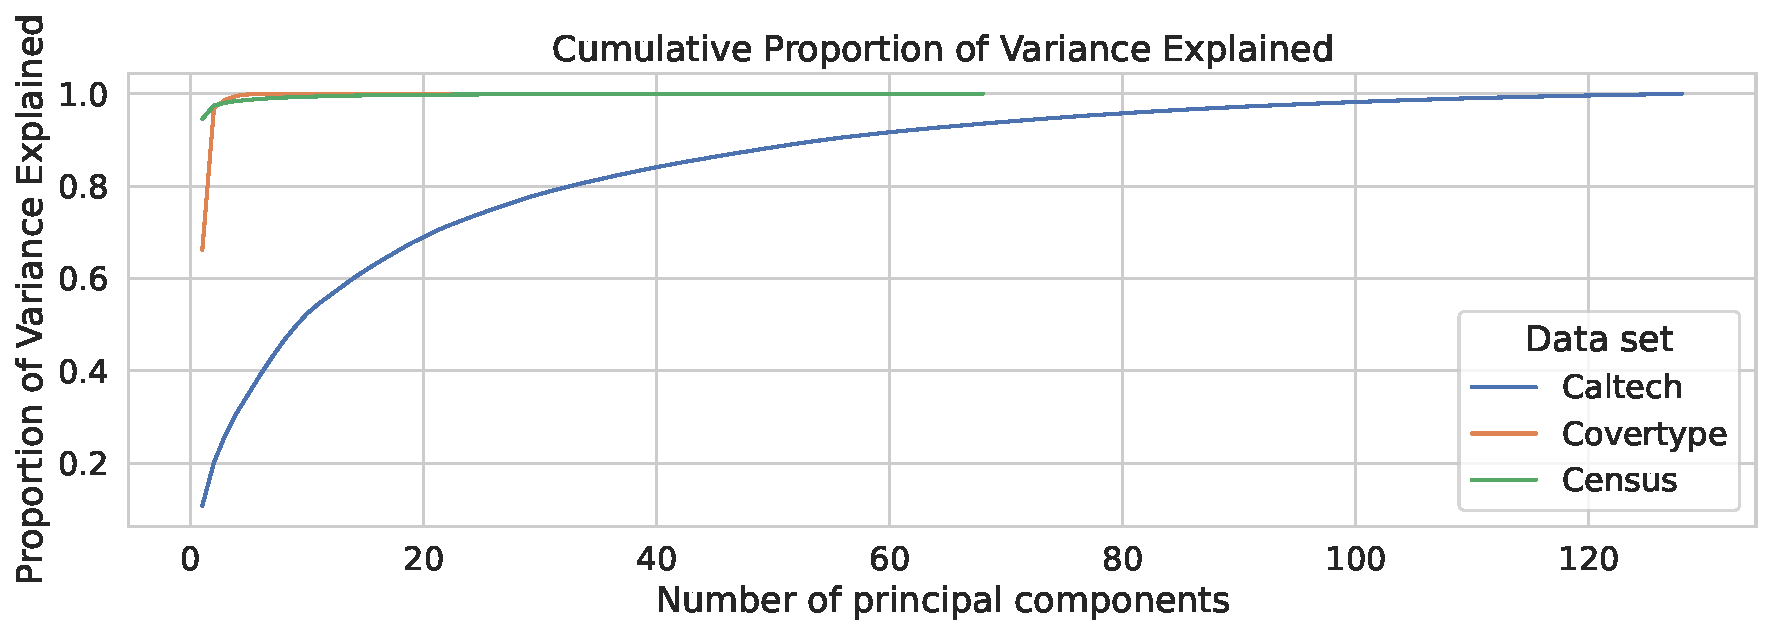
\includegraphics[width=0.9\linewidth]{figures/explained-variance-plot.pdf}
  \caption{The cumulative proportion of explained variance by principal components on \textit{Caltech}, \textit{Covertype}, and \textit{Census}.}
  \label{fig:explained-variance-pca}
\end{figure}

\begin{figure}[H]
  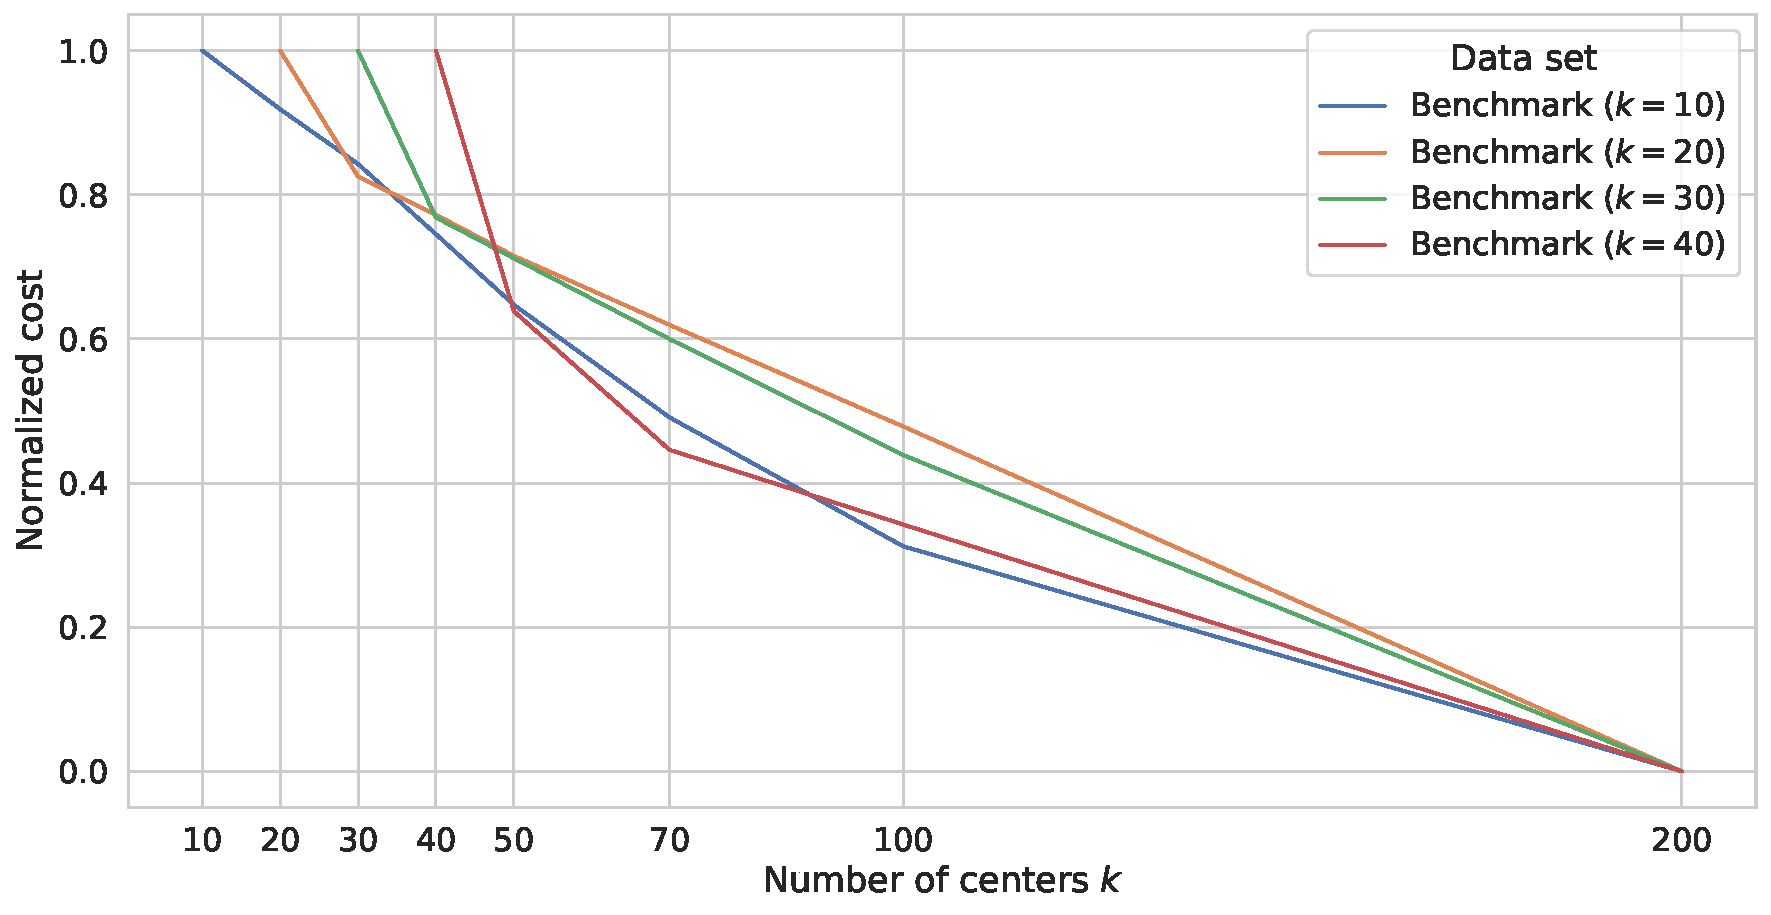
\includegraphics[width=0.9\linewidth]{figures/cost-curves-benchmark.pdf}
  \caption{Shows the clustering costs of four instances of the benchmark framework as a function of the number of centers. In contrast to real-world data sets, the costs do not decrease rapidly as more cluster centers are added.
  }
  \label{fig:cost-curves-benchmark}
\end{figure}



\newpage

\begin{figure}[H]
 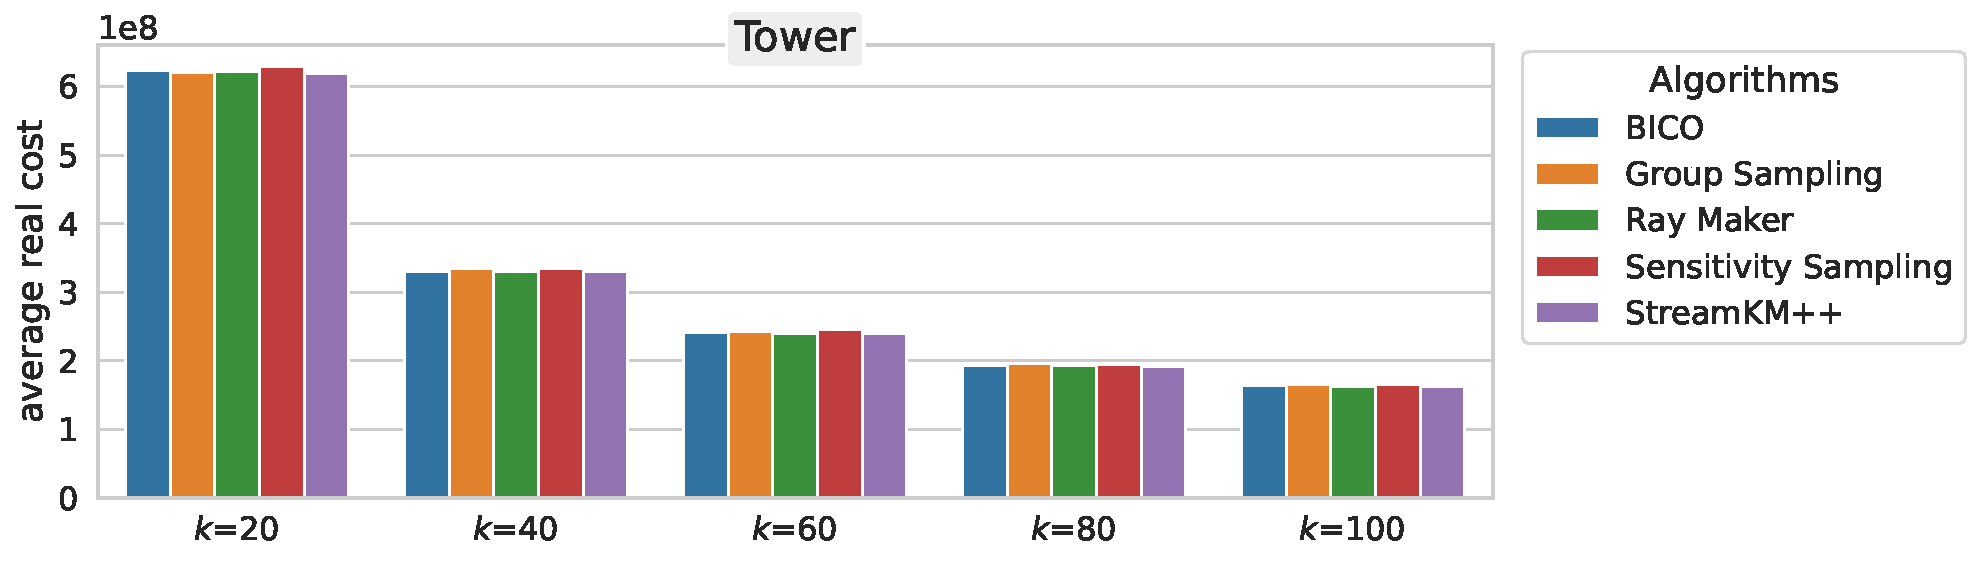
\includegraphics[width=.67\linewidth]{figures/real-costs-Tower.pdf}
 \newline
 \subfloat{
   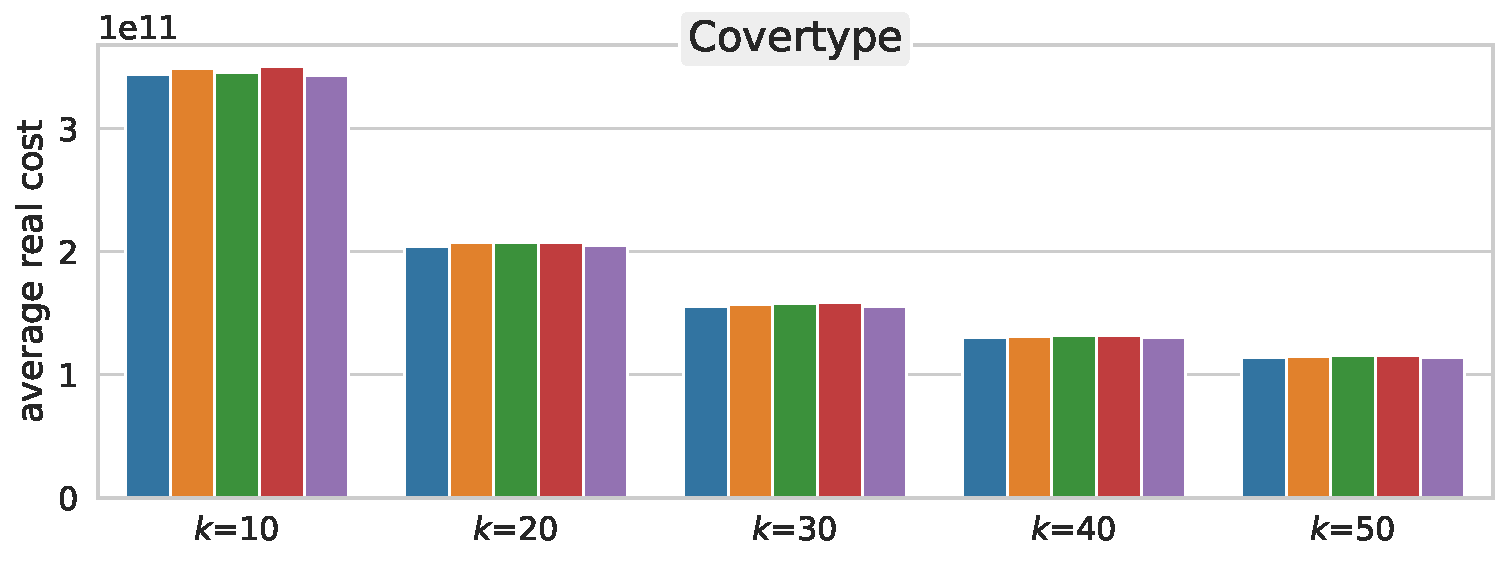
\includegraphics[width=0.5\textwidth]{figures/real-costs-Covertype.pdf}
 }
 \subfloat{
   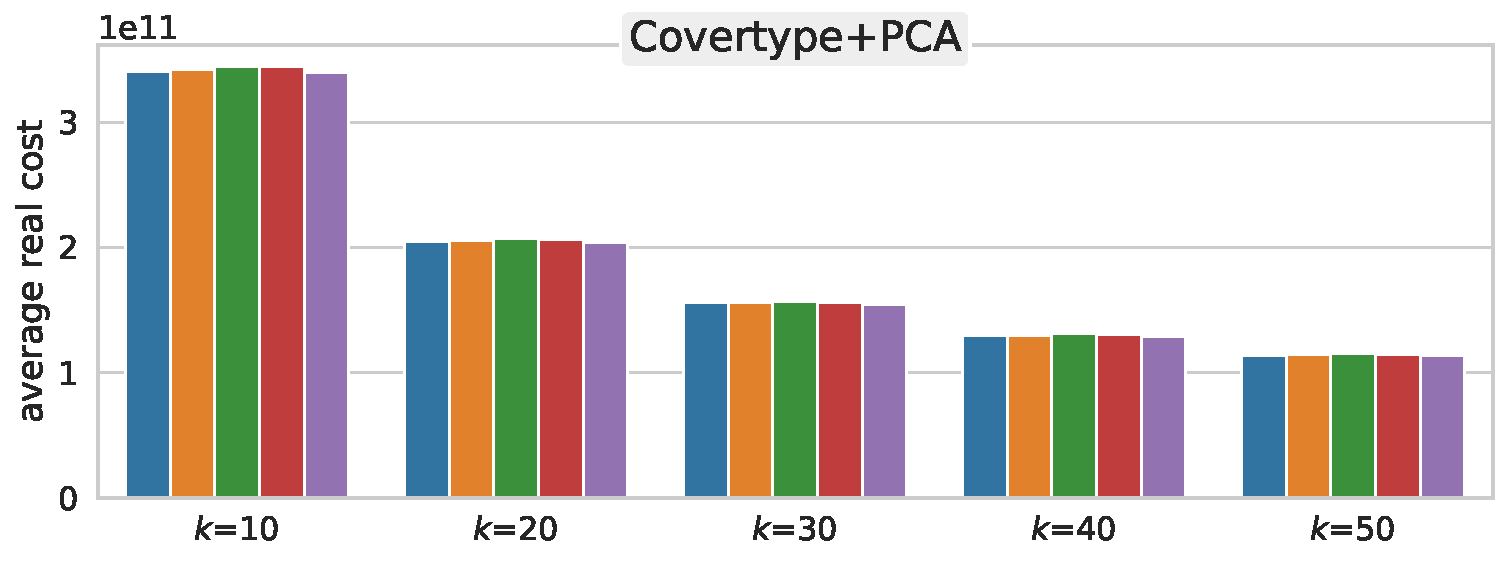
\includegraphics[width=.5\linewidth]{figures/real-costs-Covertype+PCA.pdf}
 }
 \newline\newline
 \subfloat{
   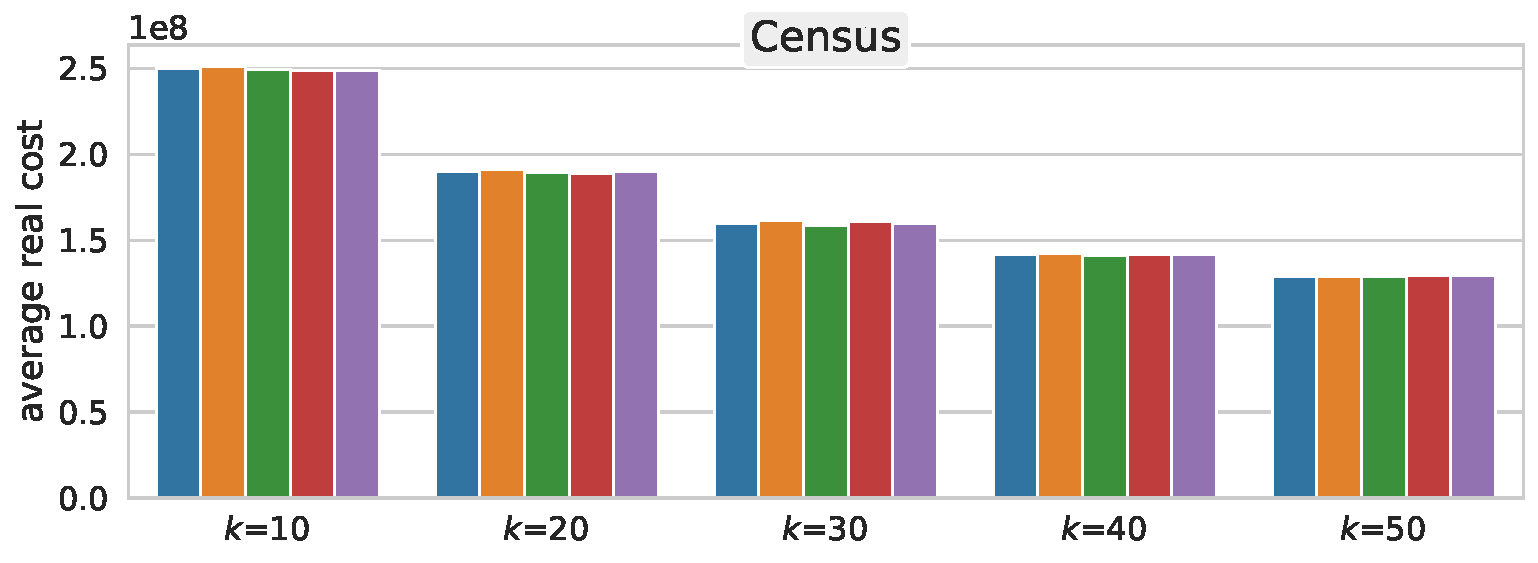
\includegraphics[width=0.5\textwidth]{figures/real-costs-Census.pdf}
 }
 \subfloat{
   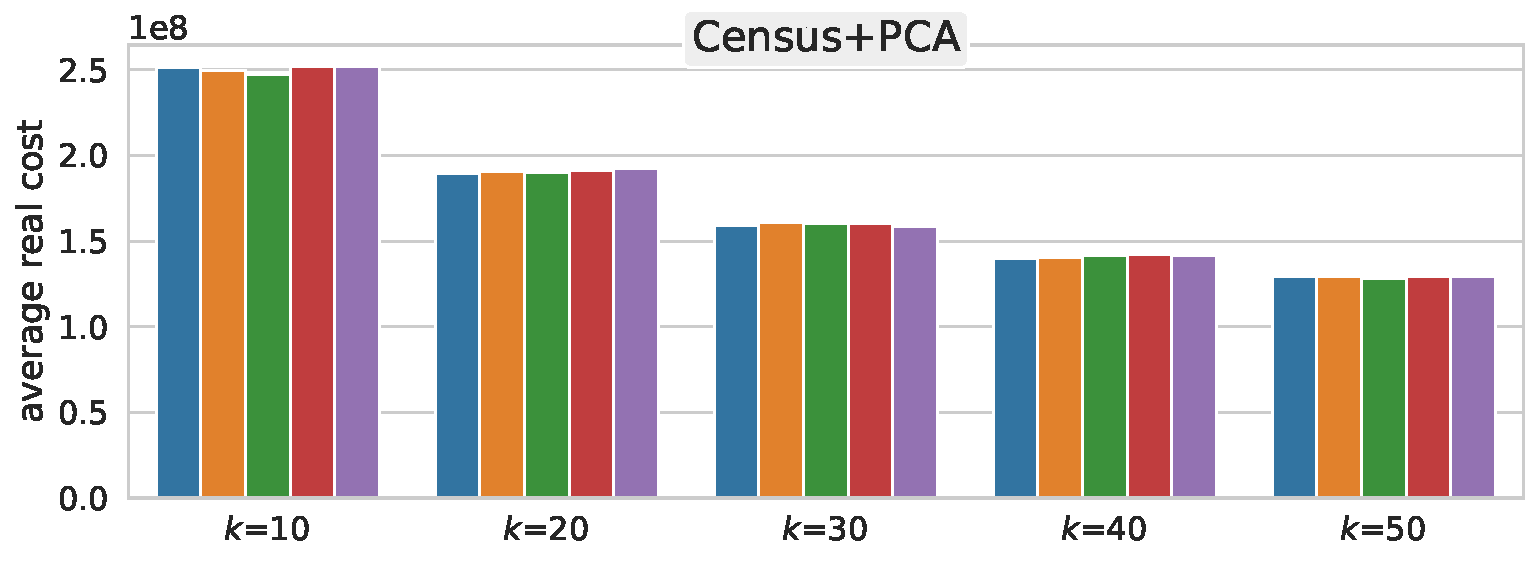
\includegraphics[width=.5\linewidth]{figures/real-costs-Census+PCA.pdf}
 }
 \newline\newline
 \subfloat{
   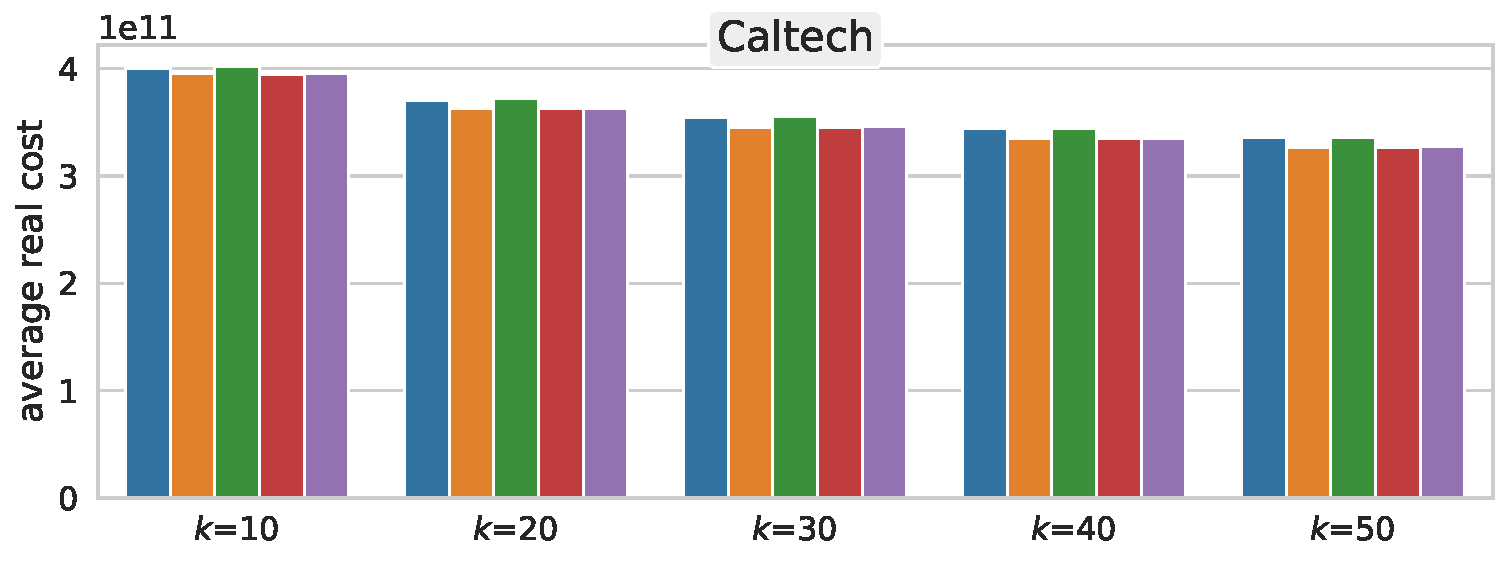
\includegraphics[width=0.5\textwidth]{figures/real-costs-Caltech.pdf}
 }
 \subfloat{
   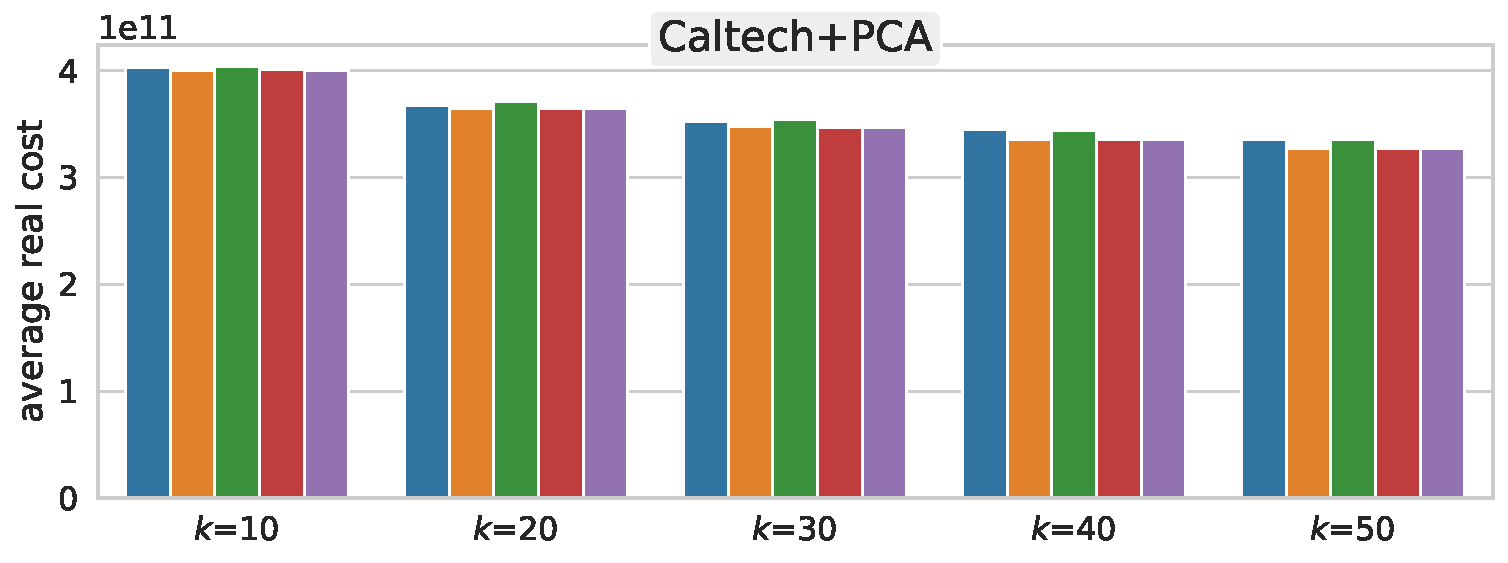
\includegraphics[width=.5\linewidth]{figures/real-costs-Caltech+PCA.pdf}
 }
 \newline\newline
 \subfloat{
   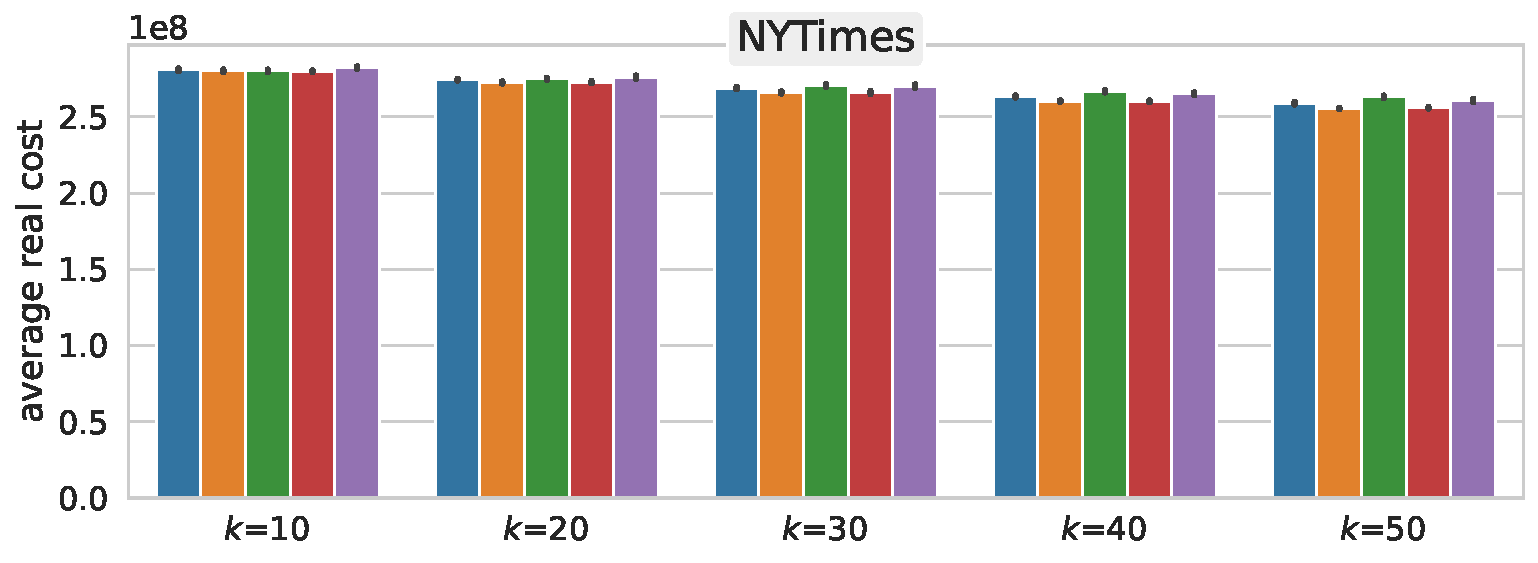
\includegraphics[width=0.5\textwidth]{figures/real-costs-NYTimes.pdf}
 }
 \subfloat{
   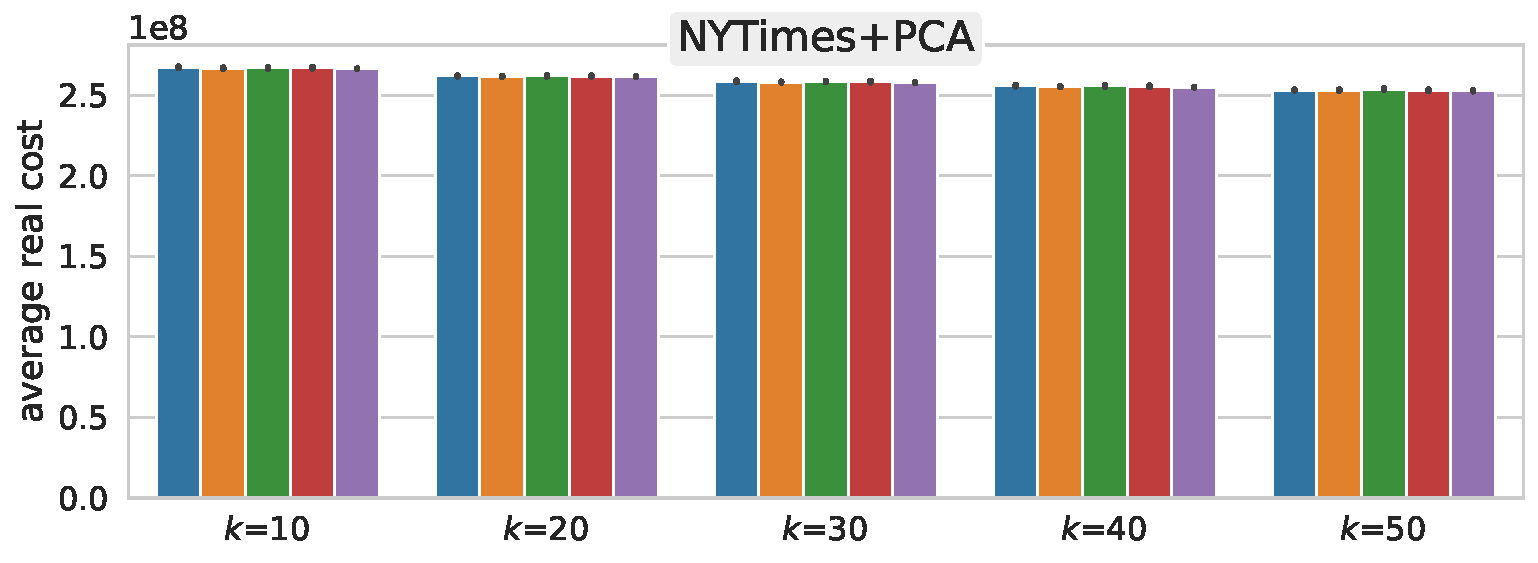
\includegraphics[width=.5\linewidth]{figures/real-costs-NYTimes+PCA.pdf}
 }
 \newline\newline
 \subfloat{
   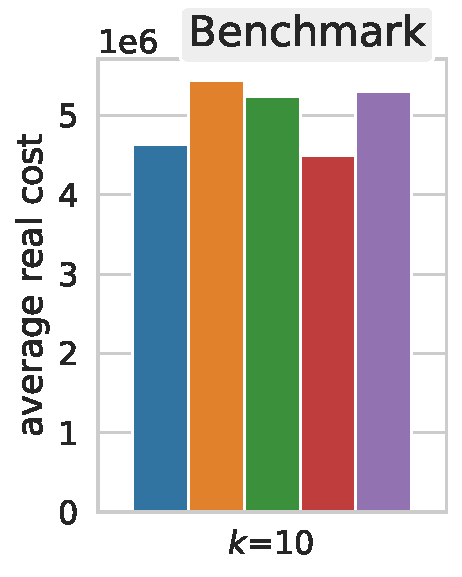
\includegraphics[width=0.15\textwidth]{figures/real-costs-Benchmark-k10.pdf}
   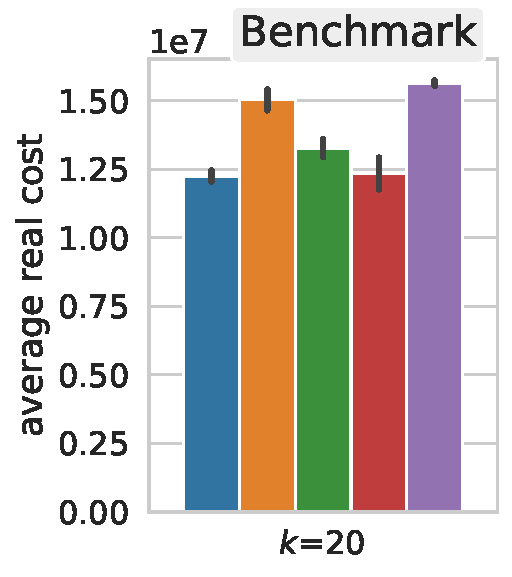
\includegraphics[width=0.165\textwidth]{figures/real-costs-Benchmark-k20.pdf}
   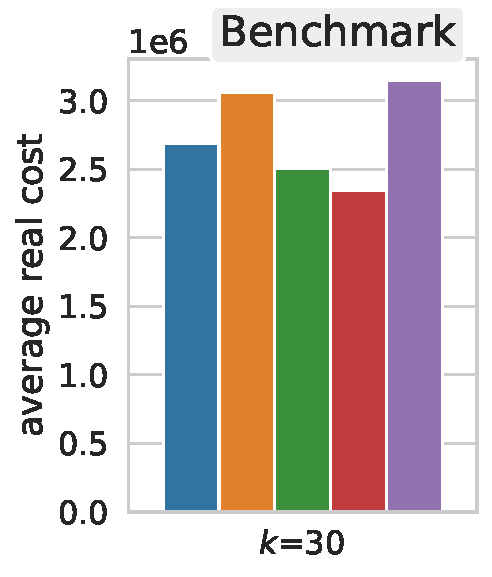
\includegraphics[width=0.16\textwidth]{figures/real-costs-Benchmark-k30.pdf}
   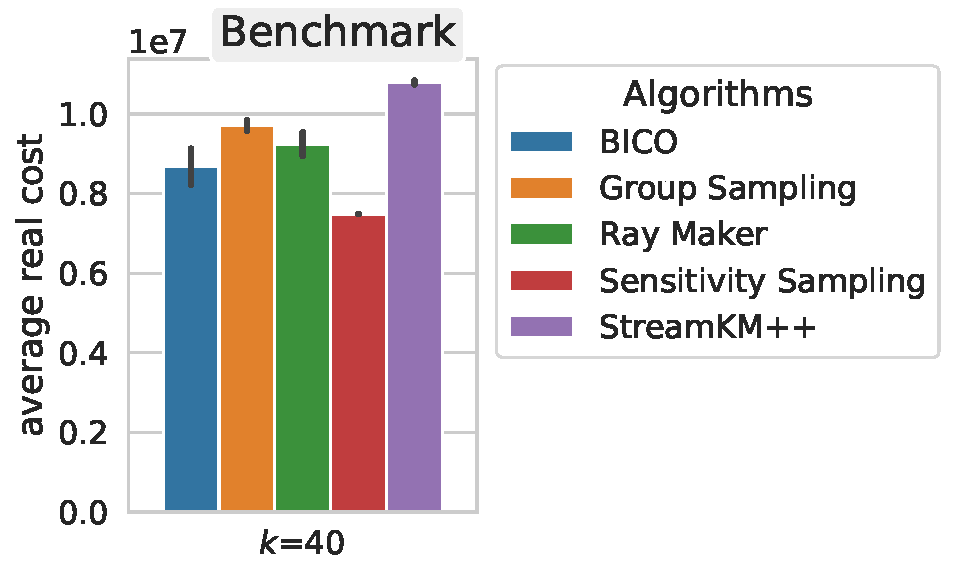
\includegraphics[width=0.31\textwidth]{figures/real-costs-Benchmark-k40.pdf}
 }
  \caption{The average costs of running the evaluated coreset algorithms multiple times on different data sets. In general, the five coreset algorithms are able to compute coresets which result in solutions with comparable costs on the different real-world data sets. The differences in cost is more noticeable on the benchmark instances. Here, Senstivity Sampling is the winner because it seems to be better at capturing the correct ``clusters'' inherent in the benchmark instances.}
 \label{fig:real-costs}
\end{figure}
